\documentclass[letterpaper, conference]{IEEEtran}

\usepackage{amsmath}
\usepackage{mathabx}
\DeclareMathOperator*{\argmax}{argmax}

\usepackage{pgfplots}
\pgfplotsset{compat=1.5.1}

\usetikzlibrary{matrix}

\setlength{\parskip}{0.7em}

\usepackage{url}

\usepackage{listings}

\usepackage{amsfonts}

\begin{document}

\title{A Discrete Bayesian Classifier \\
  \large Machine Learning Midterm Report}

\author{
  \IEEEauthorblockN{Alvaro Faundez}
  \IEEEauthorblockA{
    \textit{Master in Data Science's Program, first year student}\\
    \textit{Graduate Center, CUNY}\\
    \textit{alvaro@faundez.net}
  }
}

\maketitle

\begin{abstract}

This report details the implementation of a discrete Bayesian classifier. The classifier requirements are a class prior probabilities, the class conditional probabilities, and an Economic Gain Matrix for input. The process calculates the measurement's conditional probabilities needed for the Bayes theorem, and it outputs the Bayes decision rule, the Confusion Matrix, and the Expected Gain Matrix associated with the input used. After completing the classifications for every measurement in a testing sample set, small perturbations are introduced in the measurement conditional probabilities of every misclassification, obtaining an improvement, as expected, in the classifier's Expected Gain (after recalculating all the classifier's outputs). The experiments include the generation of synthetic random samples, and it split them equally sized testing and validation sets, or it uses V-fold Cross-Validation.

\end{abstract}

\section{Introduction}


The discrete Bayesian classifier is a popular predictive classifier broadly used in Machine Learning. It is based on the Bayes Theorem [Equation \ref{eq:bayes-theorem}].

\begin{equation}\label{eq:bayes-theorem}
  P(A \mid B) = \frac{P(B \mid A)\mathbin{}P(A)}{P(B)}
\end{equation}

A discrete Bayesian classifier, given a set of classifications and a measurement space, uses the Bayes theorem to compute the conditional probabilities and the Bayes rule decision needed to perform classifications. It can be optimized using an Economic Gain Matrix by maximizing the Expected Gain obtained using the Bayes decision rule.

In our case, given a set $C$ of $K$ discrete classifications [Equation \ref{eq:classes-set}] and a discrete measurement space $D$, result of the cartesian product of $N$ discrete measurements $L_n$ [Equation \ref{eq:measurement-space}], the classifier is a function assigning a unique classification $c \in C$ to any measurement $\vec{d} \in D$.

\begin{equation}\label{eq:classes-set}
C = \{\,c_1,\, \dots,\, c_{K}\,\}
\end{equation}


\begin{equation}\label{eq:measurement-space}
  \begin{aligned}
  L_n &= \{l_{n_1},\, \dots,\, l_{n_{M_n}}\},\, \forall n \in \{ 1, ..., N \} \\
  M_n &= \vert L_n\vert \\
  D &= \bigtimes_{n=1}^{N} L_n \\
  \end{aligned}
\end{equation}

For the classification, the following inputs are required:

\begin{itemize}
  \item the discrete classification cardinality, $K$
  \item the cardinalities of each discrete measurement, $M_n,\, n \in N$
  \item an Economic Gain Matrix, $e^{K \times K}$
  \item a dataset with $Z$ measurements with matching $Z$ classifications. 
\end{itemize}

The Economic Gain matrix, $\mathcal{E}$, is a $K \times K$ matrix that defines the gain (or cost) of making the right (or wrong) classifications [Equation \ref{eq:economic-gain-matrix}]. Each row of the matrix represents a true classification, and each column of the matrix will represent an assigned class. Then, every element $e(c_i,\, c_j) \in e$ represent the gain or cost of assigning the class $c_j$ when the true class is $c_i$. Usually, The Economic Gain has positive for every matching classification and non-positive for every other case. The identity matrix is an example of an economic gain matrix.

\begin{equation}\label{eq:economic-gain-matrix}
  \mathcal{E}^{K \times K} = \begin{pmatrix}
    e(c_1,c_1) & \cdots & e(c_1,c_K) \\
      \vdots   & \ddots &   \vdots   \\
    e(c_K,c_1) & \cdots & e(c_K,c_K)
  \end{pmatrix}
\end{equation}

The Confusion Matrix, $\mathcal{C}$ is as $K \times K$ that tells how correct is the machine learning in the classifier. Each element $P(c_i, c_j)$ in the Confusion Matrix represents the probability that the classifier assigns the classification $c_j$ when in reality the classification is $c_i$ [Equation \ref{eq:confusion-matrix}].

\begin{equation}\label{eq:confusion-matrix}
  \mathcal{C}^{K \times K} = \begin{pmatrix}
    P(c_1,c_1) & \cdots & P(c_1,c_K) \\
      \vdots   & \ddots &   \vdots   \\
    P(c_K,c_1) & \cdots & P(c_K,c_K)
  \end{pmatrix}
\end{equation}

The economical consequences of the classifier are determined by the Expected Gain Matrix $\mathcal{G}^{K \times K}$. Each element $g$ is the multiplication between the economic gain $e(i,\, j) \in K$ and the probability of the true class $c_i$ being assigned class $c_j$, $P(c_i,\, c_j)$ [Equation \ref{eq:expected-gain-matrix}].

\begin{equation}\label{eq:expected-gain-matrix}
  \mathcal{G}^{K \times K} = \begin{pmatrix}
    e(c_1,c_1)P(c_1,c_1) & \cdots & e(c_1,c_K)P(c_1,c_K) \\
              \vdots    & \ddots &            \vdots     \\
    e(c_K,c_1)P(c_K,c_1) & \cdots & e(c_K,c_K)P(c_K,c_K)
  \end{pmatrix}
\end{equation}

The classifier's Expected Gain is the sum of all the Expected Gain Matrix's elements [Equation \ref{eq:expected-gain}].

\begin{equation}\label{eq:expected-gain}
  E[e] = \sum_{i \in K} \sum_{j \in K}e(c_i,\,c_k)\mathbin{}P(c_i,\,c_k)
\end{equation}

A critical step in the construction of the classifier is the building of the Bayes decision rule $f_{\vec{d}}:C \longrightarrow \{0, 1\}, \forall \vec{d} \in D$. The goal is to determine the Bayes decision rule that maximizes the Expected Gain classifier, $E[e]$ [Equation \ref{eq:bayes-argmax}]. The Bayes decision rule will assign 1 to the class that maximizes the Expected Gain, and 0 otherwise [Equation \ref{eq:bayes-rule}].

\begin{equation}\label{eq:bayes-argmax}
  \argmax_{c_k \in C} \sum_{j = 1}^{K} e(c_j, c_k)\mathbin{}P(c_j, \vec{d})
\end{equation}

\begin{equation}\label{eq:bayes-rule}
  f_d(c_j) =
  \begin{cases}
  1 & j = k \\
  0 & j \neq k
  \end{cases}
\end{equation}

In addition to the Economic Gain Matrix, a Bayes decision rule allows a refinement of the Economic Gain definition [\label{eq:bayes-expected-gain}].

\begin{equation}\label{eq:bayes-expected-gain}
  E[e, f] = \sum_{i \in K} \sum_{j \in K}\sum_{\vec{d} \in D}f_{\vec{d}}(c_j)\mathbin{}e(c_i,\, c_j)\mathbin{}P(c_i,\,\vec{d})
\end{equation}

To obtain $f_{\vec{d}}$ and $P(c,\, \vec{d})$, it is necessary to calculate the posterior probability of assigning a class $c$ to measurement $\vec{d}$, $P(c \mid \vec{d})$, using the prior class probability $P(c)$ and the probability of the measurement given the class $P(\vec{d} \mid c)$ [Equation \ref{eq:bayes-theorem-proportional}].

\begin{equation} \label{eq:bayes-theorem-proportional}
  P(c,\, \vec{d}) \mathbin{\propto} P(\vec{d} \mid c) \mathbin{} P(c)
\end{equation}

This report details an implementation of a discrete Bayesian classifier used to implement the classifier. A technical overview explains the design and implementation, along with the results of the experiments executed.

The definition and implementation include:

\begin{itemize}
  \item Classification and measurement dimensions, including pseudo-random probabilities and cumulative distribution functions
  \item Space definition and linear addresses
  \item Class prior and conditional probabilities
  \item Classifier validation
  \item Dataset definition and generation of pseudo-random synthetic data
\end{itemize}

The classifier's performance will be measured using the Expected Gain, and it will be tested by adding small perturbations to the class conditional, increasing the Expected Gain monotonically. The process uses Test-Validation sets or V-folds Cross-Validation as validation steps.

\section{Technical}

\subsection{Definitions}

In order to explain the implementation, a few concepts need discussion.

\subsubsection{Dimension}
A dimension is a 1-dimensional set of $M$ correlatives integer numbers from 1 to $K$. Any 1-dimensional $L$ set has a Probability Mass Function $\mathbb{P}$ and a Cumulative Distribution Function $\mathbb{Q}$ [Figure \ref{fig:pmf-cdf}]. The $\mathbb{P}$ set will be created by generating a set $\mathbb{R}$ with $K$ pseudo-random numbers $r_1, ...r_K$ scaled to 1 $p_1, ...r_K$ [Equation \ref{eq:pmf}]. The $\mathbb{Q}$ set is sequence of cumulative sum of the probabilities in $\mathbb{P}$ [Equation \ref{eq:cdf}].

\pgfplotstableread[row sep=\\,col sep=&]{
value & Probability \\
1 & 0.07155134805450836 \\
2 & 0.12997048848822798 \\
3 & 0.1386944981818227 \\
4 & 0.04197817941692496 \\
5 & 0.16869281585900325 \\
6 & 0.16136757309412517 \\
7 & 0.03288486428939286 \\
8 & 0.1571494317575896 \\
9 & 0.07917145577927193 \\
10 & 0.0185393450791332 \\
}\pmf

\pgfplotstableread[row sep=\\,col sep=&]{
value & Cumulative Probability \\
1 & 0.07155134805450836 \\
2 & 0.20152183654273634 \\
3 & 0.34021633472455903 \\
4 & 0.382194514141484 \\
5 & 0.5508873300004873 \\
6 & 0.7122549030946125 \\
7 & 0.7451397673840053 \\
8 & 0.9022891991415949 \\
9 & 0.9814606549208669 \\
10 & 1.0 \\
}\cdf

\begin{figure}
  \begin{tikzpicture}
    \begin{axis}[
      ybar,
      x label style={at={(axis description cs:0.5,-0.1)}, anchor=north},
      xlabel={Dimension values},
      legend pos=north west
      ]
      \addplot table[x=value,y=Probability]{\pmf};
      \addplot table[x=value,y=Cumulative Probability]{\cdf};
      \addlegendentry{PMF}
      \addlegendentry{CDF}
    \end{axis}
  \end{tikzpicture}
  \caption{PMF and CDF values for a dimension with 10 possible values}
  \label{fig:pmf-cdf}
\end{figure}

\begin{equation}\label{eq:pmf}
  \begin{aligned}
  \mathbb{R} &= \{r_1, \dots, r_K\} \\
  \mathbb{P} &= \Bigl\{p_i \mid p_i = \frac{r_i}{r_{\sum_{i = 1}^{K} r_i}}, r_i \in \mathbb{R} \Bigr\}
  \end{aligned}
\end{equation}

\begin{equation}\label{eq:cdf}
\mathbb{Q} = \Bigl\{q_i \mid q_i = \sum_{j = 1}^{K} p_j, p_j \in \mathbb{P} \Bigr\}
\end{equation}

The classifications set $C$, and every measurement $L_n$ is a 1-dimensional set with their corresponding probabilities sets.

The cumulative distribution functions will be used to generate pseudo-random numbers in the 1-dimensional space: given a cumulative distribution function $\mathbb{Q}_n$ belonging to the dimension $M_n$, $f_{\mathbb{Q}_n}$ will take a pseudo-random number $r \in [0, 1]$. $f_{\mathbb{Q}_n}$ and assign it the number $m \in M_n$ according to the relative position of $r$ compared with the numbers in $\mathbb{Q}_n$ [Equation \ref{eq:cumulative}].

\begin{equation}\label{eq:cumulative}
  f_{\mathbb{Q}_n}(r) =
  \begin{cases}
  1 & r < q_1 \\
  m & q_{m - 1} < r \leq q_k,\, m \in M - \{1\} \\
  \end{cases}
\end{equation}

\subsubsection{Measurement Space}
The measurement space $D$ is the cartesian product of a set of $N$ measurements dimensions [Equation \ref{eq:measurement-space}]. Every element in $\vec{d} \in D$ is a vector where every value corresponds to a measurement value [Equation \ref{eq:measurements-vector}].

\begin{equation}\label{eq:measurements-vector}
  \vec{d} = (d_0, ..., d_N), \vec{d}_i \in L_n
\end{equation}

\subsubsection{Linear Space}
Each element in the measurement space can be mapped to a linear space using a bijective function $f_D$ that takes a vector and transform it to an integer value $l \in \mathcal{L}$ [Equation \ref{eq:linear-address}].

\begin{equation}\label{eq:linear-address}
  \begin{aligned}
  \mathcal{S} &= \{1,\, 2,\, 3,\, \dots,\, \prod_{i \in N} \mid L_i \mid\} \\
  f_D&: \bigtimes_{n=1}^{N} L_n \longleftrightarrow \mathcal{S} \\
  \end{aligned}
\end{equation}

Every dimension in the measurement space is independent between each other, allowing to compute the probability of every element in the measurement space $P(\vec{d})$ as the multiplication of the probabilities of each measurement value in $\vec{d}$ [Equation \ref{eq:prod:measurements}].

\begin{equation}\label{eq:prod:measurements}
  P(\vec{d}) = \prod_{i = 1}^{N} P(d_i),\, d_i \in L_i
\end{equation}

\subsubsection{Classifier}
The classifier is the function that assigns a classification to a measurement. The classifier lives in the context of a set of classifications, measurement space, and Economic Gain Matrix.

\subsubsection{Dataset}
A sample dataset is formed by two sets of equal size $Z$: the data $ X = \{x_i \in D \mid i \in [1, Z]\}$ and the target $Y = \{ y_i \in C \mid i \in [1, Z]\}$.

\subsubsection{Experiment}
An experiment is an isolated routine that takes inputs and produces results. The experiments will define dimensions, classifications, measurement space, classifier, and datasets.

An experiment uses immutable measurement space and classifications until the end of the whole process. That condition will mean that, during an experiment, the cumulative probabilities distribution of every dimension remains unchanged. The experiments will yield a classifier that will over datasets created during the experiment.

\subsubsection{Iteration}
An iteration within an experiment will enclose the use and modification of the classifier available. Each iteration in a sequence of iterations will include the classifier's changes by the previous iteration and a new dataset.

\subsubsection{Validation}
An iteration has two kinds of testing and validation processes:
\begin{itemize}
  \item Test-Validation sets: The sample dataset will be shuffled and divided into equal-sized subsets. An iteration uses the test subset to predict and adapt; the iteration finishes using the validation set [Equation \ref{eq:test-validation}].
  \item V-fold sets: The sample dataset will be shuffled and divided into $V$ equal-sized folds. A $V$ round-robin iterations will select a different fold as a validation set, and it will concatenate the resting folds as a testing set [Equation \ref{eq:v-fold}].
\end{itemize}

\begin{figure}
  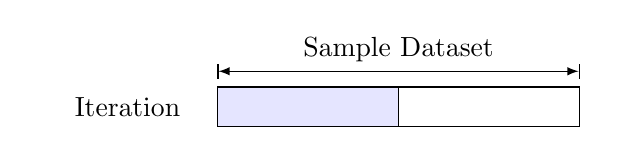
\begin{tikzpicture}
    \matrix (M) [matrix of nodes,
        nodes={minimum height = 5mm, minimum width = 2.3cm, outer sep=0, anchor=center, draw},
        column 1/.style={nodes={draw=none}, minimum width = 2.3cm},
        row sep=1mm, column sep=-\pgflinewidth, nodes in empty cells,
        e/.style={fill=blue!10}
      ]
      {
        Iteration & |[e]| & \\
      };
    \draw (M-1-2.north west) ++(0,2mm) coordinate (LT) edge[|<->|, >= latex] node[above]{Sample Dataset} (LT-|M-1-3.north east);
  \end{tikzpicture}
  \caption{Test-Validation sets, only one iteration.}
  \label{eq:test-validation}
\end{figure}

\begin{figure}\label{eq:v-fold}
  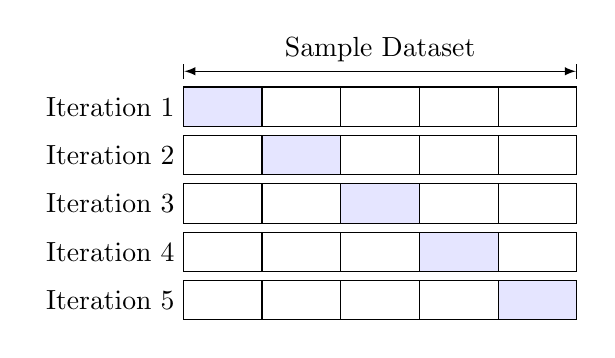
\begin{tikzpicture}
    \matrix (M) [matrix of nodes,
        nodes={minimum height = 5mm, minimum width = 1cm, outer sep=0, anchor=center, draw},
        column 1/.style={nodes={draw=none}, minimum width = 1cm},
        row sep=1mm, column sep=-\pgflinewidth, nodes in empty cells,
        e/.style={fill=blue!10}
      ]
      {
        Iteration 1 & |[e]| & & & & \\
        Iteration 2 & & |[e]| & & & \\
        Iteration 3 & & & |[e]| & & \\
        Iteration 4 & & & & |[e]| & \\
        Iteration 5 & & & & & |[e]| \\
      };
    \draw (M-1-2.north west) ++(0,2mm) coordinate (LT) edge[|<->|, >= latex] node[above]{Sample Dataset} (LT-|M-1-6.north east);
  \end{tikzpicture}
  \caption{5-fold cross-validation. Each iteration uses the blue fold as validation set and the rest folds as test set.}
\end{figure}
  

\subsection{Discrete Bayesian Classifier}

A classifier will assign a classification $c \in C$ to any measurement $\vec{d} \in D$ from the measurement space. Inside the classifier, all measurement will be translated to the corresponding linear address. The following parameters must be set during the initialization of the classifier:

\begin{itemize}
  \item The list of $S$ linear addresses $l(\vec{d})$ for each $\vec{d} \in D$ [Equation \ref{eq:linear-address}], stored in a $S$ sized vector
  \item Measurement probability $P(\vec{d})$ for each  $\vec{d} \in D$ [Equation \ref{eq:prod:measurements}], stored in a $S$ sized vector
  \item Class probability $P(c)$ for each  $c \in C$ [Equation \ref{eq:pmf}], stored in a $K$ sized vector
  \item Class conditional probabilities $P(\vec{d} \mid c)$. Each class $c \in C$ is assigned a probability mass distribution with $S$ probabilities [Equation \ref{eq:pmf}], stored in a $K \times S$ matrix
\end{itemize}

Once the classifier is ready, given an Economic Gain Matrix [Equation \ref{eq:economic-gain-matrix}], the classifier computes the values needed to classify a measurement:

\begin{itemize}
  \item $P(c \mid \vec{d})$, the probabilities of class given a measurement, stored in an $S \times K$ matrix [Equation \ref{eq:bayes-theorem}]
  \item $P(c,\, \vec{d})$ the probabilities of a class and a measurement, stored in an $S \times K$ matrix [Equation \ref{eq:bayes-theorem-proportional}]
  \item the Bayes decision rule that optimize the expected gain for the Economic Gain Matrix, stored in an $S \times K$ matrix [Equation \ref{eq:bayes-rule}]
  \item The Confusion Matrix, stored in an $K \times K$ matrix
  \item The Expected Gain Matrix, stored in an $K \times K$ matrix [Equation \ref{eq:expected-gain-matrix}]
  \item The Expected Gain, the trace of the Expected Gain Matrix
\end{itemize}

The process ends with a discrete Bayesian classifier optimized to maximize Expected Gain, given an Economic Gain Matrix.

\section{Experiment}\label{experiment}

To validate the discrete Bayesian classifier, a series of iteration will modify each measurement's probabilities given a class $P(\vec{d} \mid c$ by adding small perturbations. Each perturbation must increase the Expected Gain monotonically to 1.

Each iteration in the experiment will compute a classifier optimized for a specific Economic Gain Matrix. Using that classifier dataset of $Z$ samples measurements and corresponding classifications, it generates random measurements $\vec{d}$ assigned to random classifications $c$ using probability mass distribution $P(c \mid \vec{d})$. The sample size $Z$ will be 10 times the classifications number times the measurement space [Equation \ref{eq:sample-size}].

\begin{equation}\label{eq:sample-size}
  Z = 10 \times \mid C \mid \times \prod_{n \in N} |L_n|
\end{equation}

The classifier assigns a classification to each measurement in the test sample set. Based on those results, the conditional probabilities given a class will be modified, aiming that in the next iteration, the data generated should conform more alike to the classifications. The adaptation follows these steps:

\begin{enumerate}
  \item For each assigned classification $c'$ made, if the classification is wrong a $\Delta$ perturbation will be added to $P(\vec{d} \mid c')$\footnote{This is different to the steps defined in the midterms slides \cite{midterm-project}. Section \ref{problems} provides further information.}.
  \item Normalize to 1 each column on the $P(\vec{d} \mid c)$ matrix
  \item Compute the classifier with the new probabilities
  \item Return the Expected Gain
  \item Repeat from step 1
\end{enumerate}

Each iteration must do the same steps using the updated classifier and yield a higher Expected Gain.

\section{Experiment Results}

A base experiment will have the following default setup:

\begin{itemize}
  \item $K = 2$ classifications
  \item $N = 2$ measurements
  \item $M_n = 2, n \in N$ values for each measurement
  \item $e^{K \times K} = I_K$ as Economic Gain Matrix
  \item $\Delta = 0.01$ as a probability perturbation
  \item $R = 10$ iterations per experiment
  \item $V = 2$ folds (test/validation cross-validation)
\end{itemize}

\subsection{Default Setup}

The default case generates $Z = 80$ samples. In $R = 10$ iterations the Expected Gain goes from $0.6217987808286073$ to $0.7389581277559807$.

\subsection{Testing the Parameters}

Increasing the classifications dimension's size while keeping the rest of the default values generates a decrement in the Expected Gain [Figure \ref{fig:default-K-N2-M2-R10-D001}].

\pgfplotstableread[row sep=\\,col sep=&]{
K & EG & S & T \\
2 & 0.7389581277559807 & 80e-3 & 0.10 \\
3 & 0.6433109637953163 & 120e-3 & 0.11 \\
4 & 0.6084267457343393 & 160e-3 & 0.13 \\
5 & 0.5776429695321013 & 200e-3 & 0.14 \\
6 & 0.5837900842550331 & 240e-3 & 0.16 \\
7 & 0.5066951878117494 & 280e-3 & 0.21 \\
8 & 0.5272128049007744 & 320e-3 & 0.24 \\
9 & 0.5117121303660219 & 360e-3 & 0.29 \\
10 & 0.3578002368124974 & 400e-3 & 0.29 \\
}\expectedgainK

\begin{figure}
  \begin{tikzpicture}
    \begin{axis}[
        xtick={2,3,4,5,6,7,8,9,10},
        xlabel=Classifications cardinality $K$,
        legend pos=north east
      ]
      \addplot table[x=K,y=EG]{\expectedgainK};
      \addlegendentry{Expected Gain}
      \addplot table[x=K,y=T]{\expectedgainK};
      \addlegendentry{Time $[s]$}
      \addplot table[x=K,y=S]{\expectedgainK};
      \addlegendentry{$10^3$ samples}
    \end{axis}
  \end{tikzpicture}
  \caption{Default case: Expected Gain with different amount of classifications}
  \label{fig:default-K-N2-M2-R10-D001}
\end{figure}


Increasing the amount of measurements dimensions generates improvements on the Expected Gain but also a notorious increase of the samples generated [Figure \ref{fig:results-K2-N-M2-R10-D001}]

\pgfplotstableread[row sep=\\,col sep=&]{
N & EG & T & Z \\
2 & 0.725 & 0.12e-1 & 80e-5 \\
3 & 0.8687028064684688 & 0.14e-1 & 160e-5 \\
4 & 0.7257016986270449 & 0.29e-1 & 320e-5 \\
5 & 0.9001806721977035 & 0.46e-1 & 640e-5 \\
6 & 0.9227452080178603 & 0.62e-1 & 1280e-5 \\
7 & 0.9719919613359014 & 0.95e-1 & 2560e-5 \\
8 & 0.9812737500570743 & 1.67e-1 & 5120e-5 \\
9 & 0.9926056487661382 & 3.08e-1 & 10240e-5 \\
10 & 0.9980432439482527 & 6.16e-1 & 20480e-5 \\
}\expectedgainN

\begin{figure}
  \begin{tikzpicture}
    \begin{axis}[
        xtick={2,3,4,5,6,7,8,9, 10},
        xlabel=Measurement Space cardinality $N$,
        legend style={at={(0.25,0.6)},anchor=north},
      ]
      \addplot table[x=N,y=EG]{\expectedgainN};
      \addlegendentry{Expected Gain}
      \addplot table[x=N,y=T]{\expectedgainN};
      \addlegendentry{Time $10^{-1}[s]$}
      \addplot table[x=N,y=Z]{\expectedgainN};
      \addlegendentry{$10^{-1}$ samples}
    \end{axis}
  \end{tikzpicture}
  \caption{Default case: Expected Gain with different amount of measurement}
  \label{fig:results-K2-N-M2-R10-D001}
\end{figure}


Increasing the number of values per measurement generates improvements on the Expected Gain but also a notorious increase in the samples generated [Figure \ref{fig:results-K2-N2-M-R10-D001}]

\pgfplotstableread[row sep=\\,col sep=&]{
M & EG & T & Z \\
2 & 0.7389581277559807 & 0.15 & 80e-4 \\
3 & 0.8307953455501523 & 0.12 & 180e-4 \\
4 & 0.8200844565839027 & 0.21 & 320e-4 \\
5 & 0.8950033367636645 & 0.23 & 500e-4 \\
6 & 0.9182683425246243 & 0.34 & 720e-4 \\
7 & 0.979591836734694 & 0.38 & 980e-4 \\
8 & 0.9353759620801088 & 0.50 & 1280e-4 \\
9 & 0.9263206602702356 & 0.54 & 1620e-4 \\
10 & 0.9750271916246566 & 0.57 & 2000e-4 \\
}\expectedgainM

\begin{figure}
  \begin{tikzpicture}
    \begin{axis}[
        xtick={2,3,4,5,6,7,8,9, 10},
        xlabel=Measurement Cardinality $M$,
        legend style={at={(0.25,0.6)},anchor=north},
      ]
      \addplot table[x=M,y=EG]{\expectedgainM};
      \addlegendentry{Expected Gain}
      \addplot table[x=M,y=T]{\expectedgainM};
      \addlegendentry{Time $[s]$}
      \addplot table[x=M,y=Z]{\expectedgainM};
      \addlegendentry{$10^{-4}$ samples}
    \end{axis}
  \end{tikzpicture}
  \caption{Default case: Expected Gain with different amount of values per measurement}
  \label{fig:results-K2-N2-M-R10-D001}
\end{figure}


Using $R = 10$ iterations the Expected Gain goes from $0.6217987808286073$ to $0.7389581277559807$. For $R > 400$ the Expected Gain gets stuck in $0.8088281174549596$ [Figure \ref{fig:results-K2-N2-M2-R-D001}]

\pgfplotstableread[row sep=\\,col sep=&]{
R & EG & T & Z \\
10 & 0.7389581277559807 & 0.10e-2 & 80e-2 \\
100 & 0.8088012884426641 &  0.25e-2 & 80e-2 \\
200 &  0.8088281124010486 & 0.4e-2 & 80e-2 \\
300 & 0.8088281174539913 & 0.57e-2 & 80e-2 \\
400 & 0.8088281174549596 & 0.72e-2 & 80e-2 \\
500 & 0.8088281174549596 & 0.85e-2 & 80e-2 \\
}\expectedgainR

\begin{figure}
  \begin{tikzpicture}
    \begin{axis}[
        xtick={10,100,200,300,400,500},
        xlabel=Number of iterations $R$,
        legend style={at={(0.25,0.6)},anchor=north},
      ]
      \addplot table[x=R,y=EG]{\expectedgainR};
      \addlegendentry{Expected Gain}
      \addplot table[x=R,y=T]{\expectedgainR};
      \addlegendentry{Time $10^{-1}[s]$}
      \addplot table[x=R,y=Z]{\expectedgainR};
      \addlegendentry{$10^{-1}$ samples}
    \end{axis}
  \end{tikzpicture}
  \caption{Default case: Expected Gain with different number of iterations}
  \label{fig:results-K2-N2-M2-R-D001}
\end{figure}


The Expected Gain's increases faster using the default perturbation value $10^{-2}$ than using smaller ones [Figure \ref{fig:results-K2-N2-M2-R10-D}].

\pgfplotstableread[row sep=\\,col sep=&]{
values & P \\
0 & 0.6217987808286073 \\
1 & 0.6434589581321546 \\
2 & 0.6584925180705914 \\
3 & 0.6733906405321053 \\
4 & 0.6879017987738398 \\
5 & 0.7008581900611026 \\
6 & 0.7106736380059988 \\
7 & 0.721965746261189 \\
8 & 0.731272428889093 \\
9 & 0.7389581277559807 \\
}\expectedgaincenti

\pgfplotstableread[row sep=\\,col sep=&]{
values & P \\
0 & 0.6137987267145945 \\
1 & 0.6137987267145945 \\
2 & 0.6137987267145943 \\
3 & 0.614054830134284 \\
4 & 0.6152165593472926 \\
5 & 0.6161483510408458 \\
6 & 0.6170681848943043 \\
7 & 0.6181824597016432 \\
8 & 0.6191439887513687 \\
9 & 0.6199583837680757 \\
}\expectedgainmili

\pgfplotstableread[row sep=\\,col sep=&]{
values & P \\
0 & 0.6137987267145945 \\
1 & 0.6137987267145945 \\
2 & 0.6137987267145945 \\
3 & 0.6137987267145945 \\
4 & 0.6137987267145945 \\
5 & 0.6137987267145943 \\
6 & 0.6137987267145946 \\
7 & 0.6137987267145946 \\
8 & 0.6137987267145945 \\
9 & 0.6137987267145945 \\
}\expectedgaindecimili

\pgfplotstableread[row sep=\\,col sep=&]{
values & P \\
0 & 0.6137987267145943 \\
1 & 0.6137987267145945 \\
2 & 0.6137987267145945 \\
3 & 0.6137987267145946 \\
4 & 0.6137987267145945 \\
5 & 0.6137987267145945 \\
6 & 0.6137987267145945 \\
7 & 0.6137987267145943 \\
8 & 0.6137987267145943 \\
9 & 0.6137987267145946 \\
}\expectedgaincentimili

\begin{figure}
  \begin{tikzpicture}
    \begin{axis}[
        xtick={0,1,2,3,4,5,6,7,8,9},
        xlabel=Iteration,
        ylabel=Expected Gain,
        legend pos=north west
      ]
      \addplot table[x=values,y=P]{\expectedgaincenti};
      \addlegendentry{$\Delta = 1 \times 10^{-2}$}
      \addplot table[x=values,y=P]{\expectedgainmili};
      \addlegendentry{$\Delta = 1 \times 10^{-3}$}
      \addplot table[x=values,y=P]{\expectedgaindecimili};
      \addlegendentry{$\Delta = 1 \times 10^{-4}$}
      \addplot table[x=values,y=P]{\expectedgaincentimili};
      \addlegendentry{$\Delta = 1 \times 10^{-5}$}
    \end{axis}
  \end{tikzpicture}
  \caption{Default case: Expected Gain increasing in each iteration using different sizes of $\Delta$ perturbations}
  \label{fig:results-K2-N2-M2-R10-D}
\end{figure}


All examples discussed above use the same probabilities mass distributions when using the same values of $K$, $M$ or $L$. For example, in every case where $K = 2$ the distribution is $P(c) = \begin{pmatrix}0.6137987267145945\\0.3862012732854055\end{pmatrix}$.

\subsection{More classifications, measurements and iterations}

The measurement space size grows exponentially with the number of values in each measurement [Figure \ref{fig:results-K2-N-M2-R10-D001}]. Using $k =10$ classifications, $N = 5$ measurements each one with $M = 5$ values, the sample size has a size of $Z = 312,500$ samples. Running $R = 100$ iterations takes about $1300$ seconds, about $4000$ times the default case time for the same number of iterations. Again, the performance is better with perturbation sized $\Delta = 0.01$ [Figure \ref{fig:custom-K10-N5-M5-R100-D}].

\pgfplotstableread[row sep=\\,col sep=&]{
iteration & D001 & D0001 & D00001 \\
0 & 0.9103787224362736& 0.8365515198690241& 0.6401756051257108 \\
1 & 0.9505904769699765& 0.8795777789455559& 0.7103198293402384 \\
2 & 0.9698390295222277& 0.8931469700709691& 0.746757115765759 \\
3 & 0.9786276899909157& 0.9014464395426093& 0.7689119008947165 \\
4 & 0.9841549153122104& 0.9073813990162422& 0.7844139287381892 \\
5 & 0.9862762159796594& 0.9121348094550155& 0.795643802557085 \\
6 & 0.9891237694642169& 0.9165964144520737& 0.8045627005856608 \\
7 & 0.9910597970630248& 0.9199767811802404& 0.811537551706662 \\
8 & 0.9924123592168601& 0.9228871401232788& 0.8173636293428447 \\
9 & 0.9936287262203172& 0.9259282512299756& 0.8225105578891017 \\
10 & 0.9949182630834621 & 0.9282108684330799 & 0.8268321778673038 \\
11 & 0.9957467105003458 & 0.9303967741259093 & 0.8307371525958447 \\
12 & 0.9962825191303001 & 0.9325360593115342 & 0.8340702372997433 \\
13 & 0.9967526519072625 & 0.9345186362437969 & 0.8371751459572747 \\
14 & 0.9969173125082199 & 0.9362495068543109 & 0.8399850276683835 \\
15 & 0.9970754191893271 & 0.9378345879946055 & 0.8426198239839804 \\
16 & 0.9972552381045023 & 0.9394004892864158 & 0.8450185572235839 \\
17 & 0.997395520096149 & 0.9408834434516851 & 0.8472009672689154 \\
18 & 0.9975853883455137 & 0.9421727658878135 & 0.8494500480234173 \\
19 & 0.9976504208128822 & 0.9432967195178563 & 0.8514213326136267 \\
20 & 0.9977930638678171 & 0.9444645452411896 & 0.853223546213689 \\
21 & 0.997902338661217 & 0.9455499469547977 & 0.8549879306540256 \\
22 & 0.9979850552338184 & 0.9464563928539352 & 0.8565320169443955 \\
23 & 0.9980971473779013 & 0.947407365559023 & 0.8581416678663353 \\
24 & 0.9981736696544593 & 0.9483482574349512 & 0.859546367133692 \\
25 & 0.9982694480691746 & 0.949065762353408 & 0.8609472486833322 \\
26 & 0.9983935796169823 & 0.949903404803621 & 0.8622326491344058 \\
27 & 0.9984377560680116 & 0.9507649637435741 & 0.863493909047852 \\
28 & 0.9985097309722658 & 0.9514381798566812 & 0.8645774369010941 \\
29 & 0.9985516249728321 & 0.9521173264130434 & 0.8657340134512354 \\
30 & 0.998587825558487 & 0.9528530742024032 & 0.8667858650282206 \\
31 & 0.9986171939547892 & 0.9535193522230451 & 0.8679037416505082 \\
32 & 0.9986607736278086 & 0.954169162920856 & 0.8689602468262305 \\
33 & 0.9987072573862538 & 0.954728724763101 & 0.8698835070073467 \\
34 & 0.998733270420912 & 0.9553636769847087 & 0.8708389925726605 \\
35 & 0.998757389708289 & 0.9559091087857675 & 0.8717436463532138 \\
36 & 0.9987934615422212 & 0.956444065173321 & 0.8726387882723458 \\
37 & 0.9988445688155156 & 0.9569322811331248 & 0.8735626534291046 \\
38 & 0.9988804699726495 & 0.9574497899658927 & 0.8744010083647382 \\
39 & 0.9988970943638119 & 0.9578087345603123 & 0.8751810768343048 \\
40 & 0.9989329811201492 & 0.9582507354599066 & 0.8759601595395632 \\
41 & 0.9989485626169985 & 0.9586803924728704 & 0.8767382163917886 \\
42 & 0.9989656540472807 & 0.9590419400388834 & 0.8774789835757499 \\
43 & 0.9990085245950062 & 0.9594273968537892 & 0.8782594359049538 \\
44 & 0.9990264688997249 & 0.9598379102126733 & 0.879039101359607 \\
45 & 0.9990390874198547 & 0.960212373045338 & 0.8796337637690187 \\
46 & 0.9990532063521154 & 0.9605587092667234 & 0.8803180640018818 \\
47 & 0.9990758144828847 & 0.960899903557384 & 0.8809567617927865 \\
48 & 0.9991074468819453 & 0.9612087865797203 & 0.8815624728894106 \\
49 & 0.999121133698013 & 0.9615054561910565 & 0.8821649804842195 \\
50 & 0.9991276000749125 & 0.9619709033327362 & 0.8827864756016872 \\
51 & 0.9991391150361991 & 0.9622458351768127 & 0.8833637762591706 \\
52 & 0.9991481346834075 & 0.9625743515146952 & 0.8838866707221253 \\
53 & 0.9991557496389386 & 0.9627877516617275 & 0.8844094633797158 \\
54 & 0.9991764724100536 & 0.9630634847251236 & 0.8850029376154867 \\
55 & 0.999182939574041 & 0.9633550217502587 & 0.8855341513035857 \\
56 & 0.9991993171533082 & 0.9635828671927767 & 0.8860200986355963 \\
57 & 0.9992075716639347 & 0.9637901945833456 & 0.8865119887535072 \\
58 & 0.9992159614142396 & 0.9640630256539213 & 0.886998146799881 \\
59 & 0.9992296320872639 & 0.9643228393061921 & 0.8874835694217387 \\
60 & 0.9992366521705347 & 0.9645731802637298 & 0.8879628242880218 \\
61 & 0.9992422838836184 & 0.9648403246122503 & 0.8884164078843525 \\
62 & 0.9992558958694386 & 0.965053418440293 & 0.8888883487231772 \\
63 & 0.9992636399752286 & 0.9652810205966448 & 0.8893432736983916 \\
64 & 0.9992739316317445 & 0.9656170815079155 & 0.8897777937836107 \\
65 & 0.9992820240238806 & 0.9658349753480316 & 0.8902376441172001 \\
66 & 0.9992884108682611 & 0.9661195040689126 & 0.8906855672861623 \\
67 & 0.999300246819145 & 0.9663392887926019 & 0.8911266182188098 \\
68 & 0.9993073655621577 & 0.9665512339164644 & 0.8915712851530837 \\
69 & 0.9993202257774758 & 0.966781939613987 & 0.8919908952100655 \\
70 & 0.9993273071299869 & 0.9670147054324605 & 0.8924171471128827 \\
71 & 0.9993394967164545 & 0.9672088265796803 & 0.8928516336402299 \\
72 & 0.9993446839064264 & 0.9673879895176956 & 0.8932387509611435 \\
73 & 0.9993543410867627 & 0.9676203708536566 & 0.8936174668362489 \\
74 & 0.9993634796967901 & 0.967752641588682 & 0.8939563237081064 \\
75 & 0.9993752621145386 & 0.9679954463872859 & 0.8943684199580899 \\
76 & 0.9993944321714061 & 0.9681135586593231 & 0.8947353382085588 \\
77 & 0.9993953694007288 & 0.9682659610765744 & 0.8950936386735513 \\
78 & 0.9994030769595514 & 0.9684626142563374 & 0.8954287723958367 \\
79 & 0.9994098463921035 & 0.9686314555137354 & 0.8957392310507094 \\
80 & 0.999418266550367 & 0.9687904274817603 & 0.896098187708386 \\
81 & 0.9994223955623993 & 0.9689364247194461 & 0.8964445412344536 \\
82 & 0.9994268160744617 & 0.9690703578069291 & 0.8967582875392677 \\
83 & 0.9994350623823607 & 0.9691594811555453 & 0.8970792847544781 \\
84 & 0.9994426454050804 & 0.9693126274434841 & 0.897356207602129 \\
85 & 0.9994505215210956 & 0.9694721534141721 & 0.897697319649711 \\
86 & 0.9994560323219426 & 0.9696478524274682 & 0.8979867602967324 \\
87 & 0.9994622855656535 & 0.9697683725103495 & 0.8982973139601693 \\
88 & 0.9994641396459696 & 0.9699051438745951 & 0.8985746838362798 \\
89 & 0.9994660729439924 & 0.9700317535993452 & 0.8988562490690108 \\
90 & 0.9994690055454798 & 0.9701593919044924 & 0.8991109094833536 \\
91 & 0.9994743170539021 & 0.9703217889041673 & 0.8993760934755256 \\
92 & 0.9994786454783392 & 0.9704330470983475 & 0.8996525845395813 \\
93 & 0.9994845858562795 & 0.9705770619707706 & 0.8999263180566545 \\
94 & 0.9994957828864051 & 0.9707193609474776 & 0.900189841968887 \\
95 & 0.9994975057853984 & 0.9708482222806946 & 0.9004711671967027 \\
96 & 0.9995047202501367 & 0.9710200923093528 & 0.90077165082435 \\
97 & 0.9995063960074612 & 0.9711394635985235 & 0.9010154648895539 \\
98 & 0.9995098652928781 & 0.9712637969902449 & 0.9012744862649433 \\
99 & 0.9995150612331569 & 0.9714298100407013 & 0.9015191318191078 \\
}\expectedgain

\begin{figure}
  \begin{tikzpicture}
    \begin{axis}[
          xtick={0,25,50,75,100},
          xlabel=Iterations applied,
          ylabel=Expected Gain,
          legend pos=south east
        ]
        \addplot table[x=iteration,y=D001]{\expectedgain};
        \addlegendentry{$\Delta = 10^{-2}$}
        \addplot table[x=iteration,y=D0001]{\expectedgain};
        \addlegendentry{$\Delta = 10^{-3}$}
        \addplot table[x=iteration,y=D00001]{\expectedgain};
        \addlegendentry{$\Delta = 10^{-4}$}
    \end{axis}
  \end{tikzpicture}
  \caption{Comparing perturbation sizes with 10 classes, 5 measurements with 5 values each, 100 iterations }
  \label{fig:custom-K10-N5-M5-R100-D}
\end{figure}


Over a hundred iterations, the best Expected Gain achieved is $0.9995150612331569$, using a $\Delta = 0.01$. Over a thousand iterations, the Expected Gain raises to $0.9999999999806929$ [Figure \ref{fig:custom-K10-N5-M5-R1000-D001}].

\pgfplotstableread[row sep=\\,col sep=&]{
values & P \\
0 & 0.9250093496989441 \\
1 & 0.9780753084836921 \\
2 & 0.9951097053710133 \\
3 & 0.9974656913113211 \\
4 & 0.9992111180577127 \\
5 & 0.9996385361439233 \\
6 & 0.9999223778289434 \\
7 & 0.9999561934209628 \\
8 & 0.9999708645224802 \\
9 & 0.9999759498175925 \\
10 & 0.9999857020257312 \\
11 & 0.9999904781452945 \\
12 & 0.9999950372794086 \\
13 & 0.9999965744446331 \\
14 & 0.9999978098632097 \\
15 & 0.9999981455394199 \\
16 & 0.9999985531655615 \\
17 & 0.9999988482901137 \\
18 & 0.999999224342004 \\
19 & 0.9999995107461868 \\
20 & 0.9999996311883432 \\
21 & 0.9999997357817276 \\
22 & 0.9999997760357662 \\
23 & 0.9999998108221452 \\
24 & 0.9999998273777848 \\
25 & 0.9999998346634037 \\
26 & 0.9999998725245188 \\
27 & 0.9999998943124246 \\
28 & 0.9999999042201251 \\
29 & 0.999999919104671 \\
30 & 0.9999999332457564 \\
31 & 0.9999999376582327 \\
32 & 0.9999999455699737 \\
33 & 0.9999999523573847 \\
34 & 0.9999999551783679 \\
35 & 0.9999999590009445 \\
36 & 0.9999999655339245 \\
37 & 0.9999999692498067 \\
38 & 0.999999971392829 \\
39 & 0.999999974800207 \\
40 & 0.9999999780319175 \\
41 & 0.9999999787424634 \\
42 & 0.9999999842740135 \\
43 & 0.9999999863100272 \\
44 & 0.9999999875266761 \\
45 & 0.999999988624442 \\
46 & 0.9999999891239271 \\
47 & 0.9999999894652338 \\
48 & 0.9999999897355689 \\
49 & 0.9999999900253725 \\
50 & 0.9999999910092073 \\
51 & 0.9999999914789887 \\
52 & 0.999999992309144 \\
53 & 0.9999999927219925 \\
54 & 0.9999999930599537 \\
55 & 0.9999999931019066 \\
56 & 0.9999999945495759 \\
57 & 0.9999999945496401 \\
58 & 0.999999994691789 \\
59 & 0.9999999951266024 \\
60 & 0.999999995557955 \\
61 & 0.999999995671947 \\
62 & 0.9999999959006 \\
63 & 0.9999999959705512 \\
64 & 0.9999999962245174 \\
65 & 0.9999999963459735 \\
66 & 0.9999999964364696 \\
67 & 0.9999999965850789 \\
68 & 0.9999999969057577 \\
69 & 0.9999999969814148 \\
70 & 0.9999999972810167 \\
71 & 0.9999999974601397 \\
72 & 0.9999999974984091 \\
73 & 0.9999999976162262 \\
74 & 0.9999999977321391 \\
75 & 0.9999999977812166 \\
76 & 0.9999999978329702 \\
77 & 0.9999999979347731 \\
78 & 0.9999999980013654 \\
79 & 0.9999999980308579 \\
80 & 0.9999999980510392 \\
81 & 0.9999999980982742 \\
82 & 0.9999999981450536 \\
83 & 0.999999998161018 \\
84 & 0.9999999981947142 \\
85 & 0.9999999983502053 \\
86 & 0.9999999985144166 \\
87 & 0.9999999985757347 \\
88 & 0.9999999985857405 \\
89 & 0.9999999986086863 \\
90 & 0.9999999986200173 \\
91 & 0.9999999986309391 \\
92 & 0.9999999986309391 \\
93 & 0.9999999986638625 \\
94 & 0.99999999875755 \\
95 & 0.9999999987782776 \\
96 & 0.9999999988071244 \\
97 & 0.9999999988519772 \\
98 & 0.9999999988857275 \\
99 & 0.9999999989030582 \\
100 & 0.9999999989394605 \\
101 & 0.9999999989568767 \\
102 & 0.9999999989826189 \\
103 & 0.9999999989907485 \\
104 & 0.9999999990430943 \\
105 & 0.9999999990727508 \\
106 & 0.999999999095837 \\
107 & 0.9999999990958388 \\
108 & 0.9999999991229545 \\
109 & 0.9999999991229545 \\
110 & 0.9999999991302753 \\
111 & 0.999999999210005 \\
112 & 0.9999999992185402 \\
113 & 0.9999999992296619 \\
114 & 0.999999999234696 \\
115 & 0.9999999992504037 \\
116 & 0.9999999994579778 \\
117 & 0.9999999994701733 \\
118 & 0.999999999470174 \\
119 & 0.9999999994750451 \\
120 & 0.9999999995028533 \\
121 & 0.9999999995130079 \\
122 & 0.9999999995202954 \\
123 & 0.9999999995312472 \\
124 & 0.9999999995365014 \\
125 & 0.9999999995432634 \\
126 & 0.9999999995483012 \\
127 & 0.9999999995533426 \\
128 & 0.9999999995671041 \\
129 & 0.9999999995915072 \\
130 & 0.9999999995952834 \\
131 & 0.9999999996052235 \\
132 & 0.9999999996116116 \\
133 & 0.999999999614604 \\
134 & 0.9999999996237463 \\
135 & 0.999999999627881 \\
136 & 0.9999999996758023 \\
137 & 0.9999999996809793 \\
138 & 0.9999999996809799 \\
139 & 0.9999999996849315 \\
140 & 0.9999999997072844 \\
141 & 0.9999999997072859 \\
142 & 0.9999999997120496 \\
143 & 0.9999999997163674 \\
144 & 0.9999999997180801 \\
145 & 0.9999999997508684 \\
146 & 0.9999999997508701 \\
147 & 0.9999999997508703 \\
148 & 0.9999999997554341 \\
149 & 0.999999999757615 \\
150 & 0.9999999997634831 \\
151 & 0.999999999767319 \\
152 & 0.999999999767319 \\
153 & 0.999999999767319 \\
154 & 0.9999999997733875 \\
155 & 0.9999999997733875 \\
156 & 0.9999999997753439 \\
157 & 0.9999999997753439 \\
158 & 0.9999999997786857 \\
159 & 0.9999999997824787 \\
160 & 0.9999999997860756 \\
161 & 0.9999999997860756 \\
162 & 0.9999999997913518 \\
163 & 0.9999999998049348 \\
164 & 0.9999999998182624 \\
165 & 0.9999999998389979 \\
166 & 0.9999999998405058 \\
167 & 0.9999999998405058 \\
168 & 0.9999999998419498 \\
169 & 0.9999999998427781 \\
170 & 0.9999999998435671 \\
171 & 0.9999999998435671 \\
172 & 0.9999999998463815 \\
173 & 0.999999999849134 \\
174 & 0.9999999998505035 \\
175 & 0.9999999998530166 \\
176 & 0.9999999998530166 \\
177 & 0.9999999998530174 \\
178 & 0.9999999998636342 \\
179 & 0.9999999998656941 \\
180 & 0.9999999998677285 \\
181 & 0.9999999998689176 \\
182 & 0.999999999870103 \\
183 & 0.999999999870103 \\
184 & 0.9999999998711155 \\
185 & 0.9999999998730009 \\
186 & 0.9999999998730009 \\
187 & 0.9999999998741325 \\
188 & 0.9999999998750982 \\
189 & 0.9999999998767217 \\
190 & 0.9999999998767217 \\
191 & 0.9999999998776515 \\
192 & 0.9999999998832808 \\
193 & 0.9999999998832814 \\
194 & 0.9999999998832815 \\
195 & 0.9999999998832815 \\
196 & 0.9999999998850493 \\
197 & 0.9999999998850493 \\
198 & 0.9999999998867665 \\
199 & 0.9999999998919409 \\
200 & 0.9999999998919412 \\
201 & 0.9999999998954219 \\
202 & 0.9999999998954219 \\
203 & 0.9999999998961 \\
204 & 0.99999999989689 \\
205 & 0.9999999998976791 \\
206 & 0.9999999998976791 \\
207 & 0.9999999998983262 \\
208 & 0.9999999998989708 \\
209 & 0.9999999999002132 \\
210 & 0.9999999999028648 \\
211 & 0.9999999999040684 \\
212 & 0.9999999999049901 \\
213 & 0.9999999999072325 \\
214 & 0.9999999999072328 \\
215 & 0.999999999907981 \\
216 & 0.9999999999095157 \\
217 & 0.9999999999095156 \\
218 & 0.9999999999115458 \\
219 & 0.999999999913433 \\
220 & 0.999999999913433 \\
221 & 0.9999999999139655 \\
222 & 0.9999999999146346 \\
223 & 0.9999999999146348 \\
224 & 0.9999999999152348 \\
225 & 0.9999999999165504 \\
226 & 0.9999999999170825 \\
227 & 0.9999999999176616 \\
228 & 0.9999999999176616 \\
229 & 0.9999999999187401 \\
230 & 0.9999999999193493 \\
231 & 0.9999999999198328 \\
232 & 0.99999999992034 \\
233 & 0.9999999999208281 \\
234 & 0.9999999999247313 \\
235 & 0.999999999925191 \\
236 & 0.999999999925191 \\
237 & 0.9999999999267157 \\
238 & 0.9999999999267157 \\
239 & 0.9999999999267158 \\
240 & 0.9999999999267158 \\
241 & 0.9999999999272382 \\
242 & 0.9999999999283138 \\
243 & 0.9999999999292585 \\
244 & 0.999999999929675 \\
245 & 0.999999999929675 \\
246 & 0.999999999929675 \\
247 & 0.9999999999307247 \\
248 & 0.9999999999307247 \\
249 & 0.9999999999307247 \\
250 & 0.9999999999312272 \\
251 & 0.9999999999312272 \\
252 & 0.9999999999320799 \\
253 & 0.99999999993351 \\
254 & 0.9999999999335099 \\
255 & 0.9999999999339657 \\
256 & 0.9999999999339657 \\
257 & 0.999999999934855 \\
258 & 0.999999999934855 \\
259 & 0.9999999999353429 \\
260 & 0.9999999999357495 \\
261 & 0.9999999999361798 \\
262 & 0.9999999999361798 \\
263 & 0.9999999999361798 \\
264 & 0.9999999999361798 \\
265 & 0.999999999936614 \\
266 & 0.9999999999370311 \\
267 & 0.9999999999370311 \\
268 & 0.9999999999370311 \\
269 & 0.9999999999370311 \\
270 & 0.9999999999374461 \\
271 & 0.9999999999374461 \\
272 & 0.9999999999382319 \\
273 & 0.9999999999382317 \\
274 & 0.9999999999382319 \\
275 & 0.9999999999394589 \\
276 & 0.9999999999394589 \\
277 & 0.9999999999399021 \\
278 & 0.9999999999399021 \\
279 & 0.9999999999399021 \\
280 & 0.9999999999399021 \\
281 & 0.9999999999406779 \\
282 & 0.9999999999406778 \\
283 & 0.9999999999406779 \\
284 & 0.999999999941446 \\
285 & 0.9999999999418497 \\
286 & 0.999999999942994 \\
287 & 0.9999999999433827 \\
288 & 0.9999999999433827 \\
289 & 0.99999999994411 \\
290 & 0.9999999999448023 \\
291 & 0.9999999999448023 \\
292 & 0.9999999999451599 \\
293 & 0.99999999994516 \\
294 & 0.9999999999451599 \\
295 & 0.9999999999455014 \\
296 & 0.9999999999458226 \\
297 & 0.9999999999458226 \\
298 & 0.9999999999461296 \\
299 & 0.9999999999461296 \\
300 & 0.9999999999461296 \\
301 & 0.9999999999461296 \\
302 & 0.9999999999465048 \\
303 & 0.9999999999465048 \\
304 & 0.9999999999465048 \\
305 & 0.9999999999468632 \\
306 & 0.9999999999471556 \\
307 & 0.9999999999471556 \\
308 & 0.9999999999471556 \\
309 & 0.9999999999471556 \\
310 & 0.9999999999478035 \\
311 & 0.9999999999481135 \\
312 & 0.9999999999484557 \\
313 & 0.9999999999484557 \\
314 & 0.9999999999487803 \\
315 & 0.9999999999487803 \\
316 & 0.9999999999490898 \\
317 & 0.9999999999494577 \\
318 & 0.9999999999497358 \\
319 & 0.9999999999497358 \\
320 & 0.9999999999497358 \\
321 & 0.9999999999497358 \\
322 & 0.9999999999497358 \\
323 & 0.9999999999500311 \\
324 & 0.9999999999500311 \\
325 & 0.9999999999500311 \\
326 & 0.9999999999500311 \\
327 & 0.9999999999500311 \\
328 & 0.9999999999502968 \\
329 & 0.9999999999502966 \\
330 & 0.9999999999506473 \\
331 & 0.9999999999506473 \\
332 & 0.9999999999509827 \\
333 & 0.9999999999513071 \\
334 & 0.9999999999513071 \\
335 & 0.9999999999515599 \\
336 & 0.9999999999515599 \\
337 & 0.9999999999515599 \\
338 & 0.9999999999515599 \\
339 & 0.9999999999515599 \\
340 & 0.999999999951841 \\
341 & 0.9999999999518409 \\
342 & 0.9999999999518409 \\
343 & 0.9999999999518409 \\
344 & 0.9999999999527343 \\
345 & 0.9999999999529752 \\
346 & 0.9999999999529752 \\
347 & 0.9999999999529752 \\
348 & 0.999999999953294 \\
349 & 0.999999999953294 \\
350 & 0.999999999953294 \\
351 & 0.9999999999532939 \\
352 & 0.999999999953294 \\
353 & 0.9999999999535236 \\
354 & 0.9999999999535235 \\
355 & 0.9999999999538388 \\
356 & 0.9999999999538387 \\
357 & 0.9999999999538387 \\
358 & 0.9999999999538387 \\
359 & 0.9999999999541195 \\
360 & 0.9999999999543873 \\
361 & 0.9999999999546876 \\
362 & 0.9999999999549739 \\
363 & 0.9999999999549739 \\
364 & 0.9999999999552289 \\
365 & 0.999999999955721 \\
366 & 0.9999999999559643 \\
367 & 0.9999999999559643 \\
368 & 0.9999999999559643 \\
369 & 0.9999999999559643 \\
370 & 0.9999999999562673 \\
371 & 0.9999999999562673 \\
372 & 0.9999999999564995 \\
373 & 0.9999999999564996 \\
374 & 0.9999999999564996 \\
375 & 0.9999999999567543 \\
376 & 0.9999999999570615 \\
377 & 0.9999999999570615 \\
378 & 0.9999999999570615 \\
379 & 0.9999999999570615 \\
380 & 0.9999999999570615 \\
381 & 0.9999999999570615 \\
382 & 0.9999999999574913 \\
383 & 0.9999999999574913 \\
384 & 0.9999999999574913 \\
385 & 0.9999999999577845 \\
386 & 0.9999999999580728 \\
387 & 0.9999999999583152 \\
388 & 0.9999999999585137 \\
389 & 0.9999999999587891 \\
390 & 0.9999999999590211 \\
391 & 0.9999999999610801 \\
392 & 0.999999999961359 \\
393 & 0.9999999999613591 \\
394 & 0.9999999999613591 \\
395 & 0.999999999961359 \\
396 & 0.9999999999615234 \\
397 & 0.999999999961922 \\
398 & 0.999999999961922 \\
399 & 0.999999999961922 \\
400 & 0.9999999999626406 \\
401 & 0.9999999999626406 \\
402 & 0.9999999999626406 \\
403 & 0.9999999999626406 \\
404 & 0.9999999999629056 \\
405 & 0.9999999999629057 \\
406 & 0.999999999963115 \\
407 & 0.9999999999635708 \\
408 & 0.9999999999635708 \\
409 & 0.9999999999637704 \\
410 & 0.9999999999637704 \\
411 & 0.9999999999637704 \\
412 & 0.9999999999637704 \\
413 & 0.9999999999637704 \\
414 & 0.9999999999637704 \\
415 & 0.9999999999637704 \\
416 & 0.9999999999639689 \\
417 & 0.9999999999639689 \\
418 & 0.9999999999641586 \\
419 & 0.9999999999641586 \\
420 & 0.9999999999641586 \\
421 & 0.9999999999641586 \\
422 & 0.9999999999641586 \\
423 & 0.9999999999641586 \\
424 & 0.9999999999643379 \\
425 & 0.9999999999643381 \\
426 & 0.9999999999645304 \\
427 & 0.9999999999645306 \\
428 & 0.9999999999645308 \\
429 & 0.9999999999645308 \\
430 & 0.9999999999645308 \\
431 & 0.9999999999645308 \\
432 & 0.9999999999645308 \\
433 & 0.9999999999645308 \\
434 & 0.9999999999646871 \\
435 & 0.9999999999649045 \\
436 & 0.9999999999650857 \\
437 & 0.9999999999653372 \\
438 & 0.9999999999657576 \\
439 & 0.9999999999657576 \\
440 & 0.9999999999657576 \\
441 & 0.9999999999657576 \\
442 & 0.9999999999659647 \\
443 & 0.9999999999659647 \\
444 & 0.9999999999659646 \\
445 & 0.9999999999659647 \\
446 & 0.9999999999659647 \\
447 & 0.9999999999659647 \\
448 & 0.9999999999659647 \\
449 & 0.9999999999659647 \\
450 & 0.999999999966137 \\
451 & 0.9999999999663344 \\
452 & 0.9999999999663344 \\
453 & 0.9999999999663344 \\
454 & 0.9999999999663344 \\
455 & 0.9999999999663344 \\
456 & 0.9999999999663344 \\
457 & 0.999999999966563 \\
458 & 0.999999999966563 \\
459 & 0.999999999966563 \\
460 & 0.9999999999667807 \\
461 & 0.9999999999667807 \\
462 & 0.9999999999667808 \\
463 & 0.9999999999667809 \\
464 & 0.9999999999676973 \\
465 & 0.9999999999676975 \\
466 & 0.9999999999676976 \\
467 & 0.9999999999676976 \\
468 & 0.9999999999676976 \\
469 & 0.9999999999676976 \\
470 & 0.9999999999676976 \\
471 & 0.9999999999676976 \\
472 & 0.9999999999679052 \\
473 & 0.9999999999679052 \\
474 & 0.9999999999679052 \\
475 & 0.999999999967905 \\
476 & 0.9999999999679052 \\
477 & 0.9999999999680764 \\
478 & 0.9999999999680763 \\
479 & 0.9999999999680763 \\
480 & 0.9999999999680764 \\
481 & 0.9999999999680763 \\
482 & 0.9999999999680763 \\
483 & 0.9999999999682397 \\
484 & 0.9999999999684377 \\
485 & 0.9999999999684388 \\
486 & 0.9999999999692339 \\
487 & 0.9999999999692342 \\
488 & 0.999999999969234 \\
489 & 0.9999999999694031 \\
490 & 0.9999999999695555 \\
491 & 0.9999999999697187 \\
492 & 0.9999999999698744 \\
493 & 0.9999999999698744 \\
494 & 0.9999999999698744 \\
495 & 0.9999999999698744 \\
496 & 0.9999999999700303 \\
497 & 0.9999999999701756 \\
498 & 0.9999999999703365 \\
499 & 0.9999999999704815 \\
500 & 0.9999999999706201 \\
501 & 0.9999999999706201 \\
502 & 0.9999999999707687 \\
503 & 0.9999999999709069 \\
504 & 0.9999999999709069 \\
505 & 0.9999999999709069 \\
506 & 0.9999999999709069 \\
507 & 0.9999999999709069 \\
508 & 0.9999999999710605 \\
509 & 0.9999999999710605 \\
510 & 0.9999999999710605 \\
511 & 0.9999999999710605 \\
512 & 0.9999999999712073 \\
513 & 0.999999999971207 \\
514 & 0.9999999999712073 \\
515 & 0.999999999971207 \\
516 & 0.9999999999712071 \\
517 & 0.9999999999713473 \\
518 & 0.9999999999713473 \\
519 & 0.9999999999713473 \\
520 & 0.9999999999714888 \\
521 & 0.9999999999714888 \\
522 & 0.9999999999716364 \\
523 & 0.9999999999717777 \\
524 & 0.9999999999717777 \\
525 & 0.9999999999720596 \\
526 & 0.9999999999720596 \\
527 & 0.9999999999720596 \\
528 & 0.9999999999720596 \\
529 & 0.9999999999723259 \\
530 & 0.9999999999723258 \\
531 & 0.9999999999723259 \\
532 & 0.9999999999723259 \\
533 & 0.9999999999723259 \\
534 & 0.9999999999723259 \\
535 & 0.9999999999723259 \\
536 & 0.9999999999724544 \\
537 & 0.9999999999725858 \\
538 & 0.9999999999725858 \\
539 & 0.9999999999725858 \\
540 & 0.9999999999725858 \\
541 & 0.9999999999725859 \\
542 & 0.9999999999725859 \\
543 & 0.9999999999725858 \\
544 & 0.9999999999725858 \\
545 & 0.9999999999725858 \\
546 & 0.9999999999727258 \\
547 & 0.9999999999728484 \\
548 & 0.9999999999728484 \\
549 & 0.9999999999728483 \\
550 & 0.9999999999728484 \\
551 & 0.9999999999729768 \\
552 & 0.9999999999730994 \\
553 & 0.9999999999732162 \\
554 & 0.9999999999733415 \\
555 & 0.9999999999733414 \\
556 & 0.9999999999733414 \\
557 & 0.999999999973474 \\
558 & 0.9999999999736076 \\
559 & 0.9999999999736076 \\
560 & 0.9999999999736074 \\
561 & 0.9999999999736076 \\
562 & 0.9999999999736074 \\
563 & 0.9999999999738517 \\
564 & 0.9999999999738516 \\
565 & 0.9999999999738525 \\
566 & 0.9999999999742968 \\
567 & 0.9999999999742969 \\
568 & 0.999999999974297 \\
569 & 0.9999999999742971 \\
570 & 0.999999999974297 \\
571 & 0.999999999974297 \\
572 & 0.999999999974297 \\
573 & 0.999999999974297 \\
574 & 0.999999999974297 \\
575 & 0.999999999974297 \\
576 & 0.9999999999744135 \\
577 & 0.9999999999745404 \\
578 & 0.9999999999745403 \\
579 & 0.9999999999746514 \\
580 & 0.9999999999746513 \\
581 & 0.9999999999746514 \\
582 & 0.9999999999748709 \\
583 & 0.999999999974871 \\
584 & 0.999999999974871 \\
585 & 0.9999999999748709 \\
586 & 0.999999999974871 \\
587 & 0.9999999999748709 \\
588 & 0.9999999999748709 \\
589 & 0.9999999999748708 \\
590 & 0.9999999999748709 \\
591 & 0.9999999999748709 \\
592 & 0.9999999999748709 \\
593 & 0.9999999999748709 \\
594 & 0.9999999999748709 \\
595 & 0.9999999999748709 \\
596 & 0.9999999999748708 \\
597 & 0.9999999999748709 \\
598 & 0.9999999999748709 \\
599 & 0.9999999999749819 \\
600 & 0.999999999974982 \\
601 & 0.9999999999750829 \\
602 & 0.999999999975083 \\
603 & 0.999999999975083 \\
604 & 0.999999999975083 \\
605 & 0.999999999975083 \\
606 & 0.999999999975083 \\
607 & 0.999999999975083 \\
608 & 0.999999999975083 \\
609 & 0.999999999975083 \\
610 & 0.999999999975083 \\
611 & 0.9999999999750828 \\
612 & 0.999999999975083 \\
613 & 0.999999999975083 \\
614 & 0.9999999999751887 \\
615 & 0.9999999999752945 \\
616 & 0.9999999999752947 \\
617 & 0.9999999999752945 \\
618 & 0.9999999999752945 \\
619 & 0.9999999999752945 \\
620 & 0.9999999999752947 \\
621 & 0.9999999999752947 \\
622 & 0.9999999999752947 \\
623 & 0.9999999999761613 \\
624 & 0.9999999999761615 \\
625 & 0.9999999999761615 \\
626 & 0.9999999999761616 \\
627 & 0.9999999999761615 \\
628 & 0.9999999999761616 \\
629 & 0.9999999999762622 \\
630 & 0.9999999999762622 \\
631 & 0.9999999999762622 \\
632 & 0.9999999999762622 \\
633 & 0.9999999999762622 \\
634 & 0.9999999999762623 \\
635 & 0.9999999999762622 \\
636 & 0.9999999999762622 \\
637 & 0.9999999999762622 \\
638 & 0.9999999999763513 \\
639 & 0.9999999999763513 \\
640 & 0.9999999999763513 \\
641 & 0.9999999999763513 \\
642 & 0.9999999999763513 \\
643 & 0.999999999976459 \\
644 & 0.9999999999764589 \\
645 & 0.9999999999764589 \\
646 & 0.999999999976459 \\
647 & 0.999999999976459 \\
648 & 0.9999999999764589 \\
649 & 0.9999999999765504 \\
650 & 0.9999999999765504 \\
651 & 0.9999999999765504 \\
652 & 0.9999999999765504 \\
653 & 0.9999999999766375 \\
654 & 0.9999999999766374 \\
655 & 0.9999999999766375 \\
656 & 0.9999999999766375 \\
657 & 0.9999999999766375 \\
658 & 0.999999999976837 \\
659 & 0.999999999976837 \\
660 & 0.999999999976837 \\
661 & 0.999999999976837 \\
662 & 0.999999999976837 \\
663 & 0.999999999976837 \\
664 & 0.9999999999769463 \\
665 & 0.9999999999769463 \\
666 & 0.9999999999769463 \\
667 & 0.9999999999769463 \\
668 & 0.9999999999769463 \\
669 & 0.9999999999770489 \\
670 & 0.9999999999770488 \\
671 & 0.9999999999770489 \\
672 & 0.9999999999770489 \\
673 & 0.9999999999770489 \\
674 & 0.9999999999770489 \\
675 & 0.9999999999770489 \\
676 & 0.9999999999770489 \\
677 & 0.9999999999770489 \\
678 & 0.999999999977049 \\
679 & 0.999999999977132 \\
680 & 0.9999999999771321 \\
681 & 0.9999999999771321 \\
682 & 0.9999999999771321 \\
683 & 0.9999999999771321 \\
684 & 0.9999999999772323 \\
685 & 0.9999999999772323 \\
686 & 0.9999999999772322 \\
687 & 0.9999999999772323 \\
688 & 0.9999999999772323 \\
689 & 0.9999999999772322 \\
690 & 0.9999999999772322 \\
691 & 0.9999999999773115 \\
692 & 0.9999999999773115 \\
693 & 0.9999999999773115 \\
694 & 0.9999999999773115 \\
695 & 0.9999999999773115 \\
696 & 0.9999999999773115 \\
697 & 0.9999999999773114 \\
698 & 0.9999999999773115 \\
699 & 0.9999999999773115 \\
700 & 0.9999999999773868 \\
701 & 0.9999999999774827 \\
702 & 0.9999999999775804 \\
703 & 0.9999999999775804 \\
704 & 0.9999999999775804 \\
705 & 0.9999999999775804 \\
706 & 0.9999999999775804 \\
707 & 0.9999999999775804 \\
708 & 0.9999999999775804 \\
709 & 0.9999999999775804 \\
710 & 0.9999999999775804 \\
711 & 0.9999999999775804 \\
712 & 0.9999999999775804 \\
713 & 0.9999999999776521 \\
714 & 0.9999999999776521 \\
715 & 0.9999999999776522 \\
716 & 0.9999999999776522 \\
717 & 0.9999999999776521 \\
718 & 0.9999999999777208 \\
719 & 0.9999999999777208 \\
720 & 0.9999999999777208 \\
721 & 0.9999999999777208 \\
722 & 0.9999999999777208 \\
723 & 0.9999999999778794 \\
724 & 0.9999999999778793 \\
725 & 0.9999999999778794 \\
726 & 0.9999999999778793 \\
727 & 0.9999999999778793 \\
728 & 0.9999999999778793 \\
729 & 0.9999999999778793 \\
730 & 0.9999999999779833 \\
731 & 0.9999999999780724 \\
732 & 0.9999999999780724 \\
733 & 0.9999999999780724 \\
734 & 0.9999999999781715 \\
735 & 0.9999999999781715 \\
736 & 0.9999999999781715 \\
737 & 0.9999999999782565 \\
738 & 0.9999999999782565 \\
739 & 0.9999999999782565 \\
740 & 0.9999999999783515 \\
741 & 0.9999999999783517 \\
742 & 0.9999999999783517 \\
743 & 0.9999999999783517 \\
744 & 0.9999999999783517 \\
745 & 0.9999999999783517 \\
746 & 0.9999999999783517 \\
747 & 0.9999999999783517 \\
748 & 0.9999999999783517 \\
749 & 0.9999999999783517 \\
750 & 0.9999999999783517 \\
751 & 0.9999999999785336 \\
752 & 0.9999999999785336 \\
753 & 0.9999999999785336 \\
754 & 0.9999999999785336 \\
755 & 0.9999999999785336 \\
756 & 0.9999999999786828 \\
757 & 0.9999999999786828 \\
758 & 0.9999999999786828 \\
759 & 0.9999999999786828 \\
760 & 0.9999999999786826 \\
761 & 0.9999999999786828 \\
762 & 0.9999999999786828 \\
763 & 0.9999999999786826 \\
764 & 0.9999999999786828 \\
765 & 0.9999999999786828 \\
766 & 0.9999999999787639 \\
767 & 0.9999999999787639 \\
768 & 0.9999999999787639 \\
769 & 0.9999999999787639 \\
770 & 0.999999999978823 \\
771 & 0.9999999999788232 \\
772 & 0.9999999999789031 \\
773 & 0.9999999999789031 \\
774 & 0.9999999999789031 \\
775 & 0.9999999999789031 \\
776 & 0.9999999999789031 \\
777 & 0.9999999999789031 \\
778 & 0.9999999999789031 \\
779 & 0.9999999999789031 \\
780 & 0.9999999999789031 \\
781 & 0.9999999999789031 \\
782 & 0.9999999999789031 \\
783 & 0.9999999999789031 \\
784 & 0.9999999999789031 \\
785 & 0.9999999999789031 \\
786 & 0.9999999999790568 \\
787 & 0.9999999999790568 \\
788 & 0.9999999999790568 \\
789 & 0.9999999999790568 \\
790 & 0.9999999999790568 \\
791 & 0.9999999999790568 \\
792 & 0.9999999999790568 \\
793 & 0.9999999999790568 \\
794 & 0.9999999999791132 \\
795 & 0.9999999999791132 \\
796 & 0.9999999999791132 \\
797 & 0.9999999999791132 \\
798 & 0.9999999999791132 \\
799 & 0.9999999999791132 \\
800 & 0.9999999999791132 \\
801 & 0.9999999999791669 \\
802 & 0.999999999979167 \\
803 & 0.999999999979167 \\
804 & 0.999999999979167 \\
805 & 0.999999999979167 \\
806 & 0.999999999979167 \\
807 & 0.999999999979167 \\
808 & 0.999999999979167 \\
809 & 0.999999999979167 \\
810 & 0.999999999979167 \\
811 & 0.9999999999792534 \\
812 & 0.9999999999792534 \\
813 & 0.9999999999792534 \\
814 & 0.9999999999792534 \\
815 & 0.9999999999792533 \\
816 & 0.9999999999792534 \\
817 & 0.9999999999792534 \\
818 & 0.9999999999792534 \\
819 & 0.9999999999792534 \\
820 & 0.9999999999793476 \\
821 & 0.9999999999793475 \\
822 & 0.9999999999793475 \\
823 & 0.9999999999793477 \\
824 & 0.9999999999793475 \\
825 & 0.9999999999793475 \\
826 & 0.9999999999793475 \\
827 & 0.9999999999793475 \\
828 & 0.9999999999793477 \\
829 & 0.9999999999793475 \\
830 & 0.9999999999793476 \\
831 & 0.9999999999795035 \\
832 & 0.999999999979586 \\
833 & 0.9999999999795861 \\
834 & 0.9999999999795861 \\
835 & 0.9999999999795861 \\
836 & 0.9999999999795861 \\
837 & 0.999999999979716 \\
838 & 0.999999999979716 \\
839 & 0.999999999979716 \\
840 & 0.999999999979716 \\
841 & 0.999999999979716 \\
842 & 0.999999999979716 \\
843 & 0.999999999979716 \\
844 & 0.9999999999797162 \\
845 & 0.999999999979716 \\
846 & 0.999999999979716 \\
847 & 0.999999999979716 \\
848 & 0.999999999979716 \\
849 & 0.999999999979716 \\
850 & 0.999999999979716 \\
851 & 0.999999999979716 \\
852 & 0.999999999979716 \\
853 & 0.999999999979716 \\
854 & 0.999999999979716 \\
855 & 0.999999999979716 \\
856 & 0.999999999979716 \\
857 & 0.999999999979716 \\
858 & 0.999999999979716 \\
859 & 0.9999999999798059 \\
860 & 0.9999999999798059 \\
861 & 0.9999999999798057 \\
862 & 0.9999999999798059 \\
863 & 0.9999999999798059 \\
864 & 0.9999999999798059 \\
865 & 0.9999999999798057 \\
866 & 0.9999999999798059 \\
867 & 0.9999999999798059 \\
868 & 0.9999999999798059 \\
869 & 0.9999999999798783 \\
870 & 0.9999999999798785 \\
871 & 0.9999999999798783 \\
872 & 0.9999999999798783 \\
873 & 0.9999999999798785 \\
874 & 0.9999999999798783 \\
875 & 0.9999999999798783 \\
876 & 0.9999999999798783 \\
877 & 0.9999999999798783 \\
878 & 0.9999999999799485 \\
879 & 0.9999999999799485 \\
880 & 0.9999999999799485 \\
881 & 0.9999999999799485 \\
882 & 0.9999999999799485 \\
883 & 0.9999999999799485 \\
884 & 0.9999999999799485 \\
885 & 0.9999999999799485 \\
886 & 0.9999999999799485 \\
887 & 0.9999999999799485 \\
888 & 0.9999999999799485 \\
889 & 0.9999999999799485 \\
890 & 0.9999999999799485 \\
891 & 0.9999999999799485 \\
892 & 0.9999999999799485 \\
893 & 0.9999999999799485 \\
894 & 0.9999999999799485 \\
895 & 0.9999999999799485 \\
896 & 0.9999999999799485 \\
897 & 0.9999999999799485 \\
898 & 0.9999999999799485 \\
899 & 0.9999999999799485 \\
900 & 0.9999999999799485 \\
901 & 0.9999999999799485 \\
902 & 0.9999999999799485 \\
903 & 0.9999999999799485 \\
904 & 0.9999999999799485 \\
905 & 0.9999999999799485 \\
906 & 0.9999999999799485 \\
907 & 0.9999999999799485 \\
908 & 0.9999999999799485 \\
909 & 0.9999999999799485 \\
910 & 0.9999999999799485 \\
911 & 0.9999999999799485 \\
912 & 0.9999999999799485 \\
913 & 0.9999999999799485 \\
914 & 0.9999999999799485 \\
915 & 0.9999999999799485 \\
916 & 0.9999999999799485 \\
917 & 0.9999999999799485 \\
918 & 0.9999999999799485 \\
919 & 0.9999999999799485 \\
920 & 0.9999999999799485 \\
921 & 0.9999999999799485 \\
922 & 0.9999999999799485 \\
923 & 0.9999999999799485 \\
924 & 0.9999999999799485 \\
925 & 0.9999999999799485 \\
926 & 0.9999999999799485 \\
927 & 0.9999999999799485 \\
928 & 0.9999999999799485 \\
929 & 0.9999999999799485 \\
930 & 0.9999999999799485 \\
931 & 0.9999999999799485 \\
932 & 0.9999999999799485 \\
933 & 0.999999999980034 \\
934 & 0.999999999980034 \\
935 & 0.999999999980034 \\
936 & 0.999999999980034 \\
937 & 0.999999999980034 \\
938 & 0.999999999980034 \\
939 & 0.999999999980034 \\
940 & 0.999999999980034 \\
941 & 0.999999999980034 \\
942 & 0.999999999980034 \\
943 & 0.999999999980034 \\
944 & 0.999999999980034 \\
945 & 0.999999999980034 \\
946 & 0.999999999980034 \\
947 & 0.999999999980034 \\
948 & 0.999999999980034 \\
949 & 0.999999999980034 \\
950 & 0.999999999980034 \\
951 & 0.9999999999800828 \\
952 & 0.9999999999800828 \\
953 & 0.9999999999800827 \\
954 & 0.9999999999800828 \\
955 & 0.9999999999801613 \\
956 & 0.9999999999801612 \\
957 & 0.9999999999801612 \\
958 & 0.9999999999801611 \\
959 & 0.9999999999802427 \\
960 & 0.9999999999803174 \\
961 & 0.9999999999803174 \\
962 & 0.9999999999803952 \\
963 & 0.9999999999803952 \\
964 & 0.9999999999803952 \\
965 & 0.9999999999803951 \\
966 & 0.9999999999803952 \\
967 & 0.9999999999804619 \\
968 & 0.9999999999804619 \\
969 & 0.9999999999804619 \\
970 & 0.9999999999804619 \\
971 & 0.9999999999804619 \\
972 & 0.9999999999804619 \\
973 & 0.9999999999805332 \\
974 & 0.9999999999805798 \\
975 & 0.9999999999805798 \\
976 & 0.9999999999805798 \\
977 & 0.9999999999805798 \\
978 & 0.9999999999805798 \\
979 & 0.9999999999806487 \\
980 & 0.9999999999806487 \\
981 & 0.9999999999806487 \\
982 & 0.9999999999806487 \\
983 & 0.9999999999806487 \\
984 & 0.9999999999806487 \\
985 & 0.9999999999806487 \\
986 & 0.9999999999806487 \\
987 & 0.9999999999806487 \\
988 & 0.9999999999806487 \\
989 & 0.9999999999806487 \\
990 & 0.9999999999806929 \\
991 & 0.9999999999806929 \\
992 & 0.9999999999806928 \\
993 & 0.9999999999806929 \\
994 & 0.9999999999806929 \\
995 & 0.9999999999806929 \\
996 & 0.9999999999806929 \\
997 & 0.9999999999806929 \\
998 & 0.9999999999806929 \\
999 & 0.9999999999806929 \\
}\expectedgain

\begin{figure}
  \begin{tikzpicture}
    \begin{axis}[
        xlabel=Iterations applied,
        ylabel=Expected Gain,
      ]
      \addplot table[x=values,y=P]{\expectedgain};
    \end{axis}
  \end{tikzpicture}
  \caption{$1000$ iterations with $10$ classes, $5$ measurements (each with $5$ values), and perturbation $0.01$}
  \label{fig:custom-K10-N5-M5-R1000-D001}
\end{figure}



\subsubsection{V-fold cross-validation}

All the previous experiments divided the sample set into a test set and a validation set. V-fold Cross-Validation allows using more data for the testing, producing better results in fewer iterations [Figure \ref{fig:custom-K6-N4-M3-R1000-D001-V}].

\pgfplotstableread[row sep=\\,col sep=&]{
iteration & EG \\
0 & 0.7663791706964068 \\
1 & 0.8246564213394958 \\
2 & 0.8459724494828318 \\
3 & 0.8615896590595276 \\
4 & 0.8721218869483157 \\
5 & 0.8789064707995186 \\
6 & 0.8834940325116285 \\
7 & 0.8881081975581829 \\
8 & 0.890819138949982 \\
9 & 0.8936608887826926 \\
10 & 0.8974029981717129 \\
11 & 0.8984099648225878 \\
12 & 0.9015460045983431 \\
13 & 0.9043066026452047 \\
14 & 0.9053633158343029 \\
15 & 0.9069708112016388 \\
16 & 0.9073383784237801 \\
17 & 0.9082674376376262 \\
18 & 0.9099675147904168 \\
19 & 0.9122946859902701 \\
20 & 0.9135294293799491 \\
21 & 0.9153445190408944 \\
22 & 0.9166306336427021 \\
23 & 0.918337516430839 \\
24 & 0.9198289360305674 \\
25 & 0.9212084498428622 \\
26 & 0.9222224939367738 \\
27 & 0.9228844443595432 \\
28 & 0.9236859652993211 \\
29 & 0.9248728212214581 \\
30 & 0.9255794783494837 \\
31 & 0.9262590099986234 \\
32 & 0.9275142159674442 \\
33 & 0.9281302612749072 \\
34 & 0.9288274304514137 \\
35 & 0.9292744160841746 \\
36 & 0.9301785070964504 \\
37 & 0.9305916483630803 \\
38 & 0.9310834701118296 \\
39 & 0.931640151476282 \\
40 & 0.9327971297380911 \\
41 & 0.9332062310895242 \\
42 & 0.9334445401223094 \\
43 & 0.9337500603778888 \\
44 & 0.9339725246732788 \\
45 & 0.9341885053037111 \\
46 & 0.9351245115399109 \\
47 & 0.9353832795111935 \\
48 & 0.935806484212607 \\
49 & 0.9360390150199216 \\
50 & 0.936419310445948 \\
51 & 0.9366780189365781 \\
52 & 0.9368770243573936 \\
53 & 0.9371586325664156 \\
54 & 0.9373391518880353 \\
55 & 0.9375540541947318 \\
56 & 0.9377587218992443 \\
57 & 0.9378389848951403 \\
58 & 0.938066141031187 \\
59 & 0.9383465798806396 \\
60 & 0.9384486818865705 \\
61 & 0.9386107477789496 \\
62 & 0.9387650962829445 \\
63 & 0.9388256252614816 \\
64 & 0.9389697413237282 \\
65 & 0.9391583041919764 \\
66 & 0.9393107809666313 \\
67 & 0.9394085225040529 \\
68 & 0.9395248813734971 \\
69 & 0.9400748440212019 \\
70 & 0.9406372965652497 \\
71 & 0.9408132601359308 \\
72 & 0.9409239290699037 \\
73 & 0.9410605573536073 \\
74 & 0.9411572283044216 \\
75 & 0.9412484272992967 \\
76 & 0.9413344640895814 \\
77 & 0.9413762295276598 \\
78 & 0.9414550322258607 \\
79 & 0.9415055467750519 \\
80 & 0.9415303088121529 \\
81 & 0.9415779281064589 \\
82 & 0.9416346177412978 \\
83 & 0.9416782251521891 \\
84 & 0.9416996013357715 \\
85 & 0.9417695234237207 \\
86 & 0.9417891094438173 \\
87 & 0.9418267748654732 \\
88 & 0.9418629916166505 \\
89 & 0.9418978154156346 \\
90 & 0.941931299837684 \\
91 & 0.9424070646588223 \\
92 & 0.9424672667831809 \\
93 & 0.9424820222060984 \\
94 & 0.9425429390883884 \\
95 & 0.942575170243154 \\
96 & 0.942605866580935 \\
97 & 0.9426294791484929 \\
98 & 0.9426628931591008 \\
99 & 0.9426791135526641 \\
100 & 0.9427191639069122 \\
101 & 0.942728980170258 \\
102 & 0.9427432756993565 \\
103 & 0.9427432756994079 \\
104 & 0.9427659670153843 \\
105 & 0.9427791852577021 \\
106 & 0.9427920185026807 \\
107 & 0.9428004062445026 \\
108 & 0.942812621402478 \\
109 & 0.9428166528077537 \\
110 & 0.942839472082854 \\
111 & 0.942850549400869 \\
112 & 0.9428810374320848 \\
113 & 0.9428909041088585 \\
114 & 0.9433504675167041 \\
115 & 0.9433596783800065 \\
116 & 0.9433797643747445 \\
117 & 0.9433934283167431 \\
118 & 0.9433987867253709 \\
119 & 0.9434115448411485 \\
120 & 0.9434213587763621 \\
121 & 0.9434416168995087 \\
122 & 0.9434438455159171 \\
123 & 0.9434564603257725 \\
124 & 0.9434702147913465 \\
125 & 0.9434880777336505 \\
126 & 0.9434965838966526 \\
127 & 0.9435046850042736 \\
128 & 0.9435124003448649 \\
129 & 0.9435183352222429 \\
130 & 0.943518335222243 \\
131 & 0.9435212444758597 \\
132 & 0.9435307607260074 \\
133 & 0.9435307607260074 \\
134 & 0.9435372343655637 \\
135 & 0.9435422140882993 \\
136 & 0.9435458401 \\
137 & 0.943548210042288 \\
138 & 0.9435527676236111 \\
139 & 0.9435571499133448 \\
140 & 0.9435613636534734 \\
141 & 0.9435654153266739 \\
142 & 0.9435737788722715 \\
143 & 0.9435782040286723 \\
144 & 0.9435807817896825 \\
145 & 0.9435848734738255 \\
146 & 0.9435864780558424 \\
147 & 0.9435910193257016 \\
148 & 0.9435932238256333 \\
149 & 0.9435980311463565 \\
150 & 0.9436006725313693 \\
151 & 0.9436013263395406 \\
152 & 0.9436067247556355 \\
153 & 0.9436106488379473 \\
154 & 0.9436133182816968 \\
155 & 0.9436163402934888 \\
156 & 0.9436191912480095 \\
157 & 0.9436205752065148 \\
158 & 0.9436231864489774 \\
159 & 0.9436252588636302 \\
160 & 0.9436268530287478 \\
161 & 0.9436283858798223 \\
162 & 0.9436305550087016 \\
163 & 0.9436329201024951 \\
164 & 0.9436351304705264 \\
165 & 0.9436366341222484 \\
166 & 0.9436377907774192 \\
167 & 0.943638633002058 \\
168 & 0.9436391834756782 \\
169 & 0.9436402420787939 \\
170 & 0.94364197343903 \\
171 & 0.9440860804656225 \\
172 & 0.9440863093331866 \\
173 & 0.9440873991787301 \\
174 & 0.9440893807160822 \\
175 & 0.9440911821136748 \\
176 & 0.9440923605980813 \\
177 & 0.9440931622881537 \\
178 & 0.9440939258025084 \\
179 & 0.9440946529590366 \\
180 & 0.944096211151597 \\
181 & 0.944096589353675 \\
182 & 0.9440969565401582 \\
183 & 0.94409742729206 \\
184 & 0.9440979877109905 \\
185 & 0.9440986221475156 \\
186 & 0.9440993139007362 \\
187 & 0.9440999603990732 \\
188 & 0.9441003156179397 \\
189 & 0.9441006571745421 \\
190 & 0.9441008246042492 \\
191 & 0.9441012984619106 \\
192 & 0.9441016022168218 \\
193 & 0.9441017511162879 \\
194 & 0.9441020374614155 \\
195 & 0.9441023127932688 \\
196 & 0.9441025775354355 \\
197 & 0.9441028320952112 \\
198 & 0.944103017454271 \\
199 & 0.9441031386039834 \\
200 & 0.9441035873066218 \\
201 & 0.9441039542363494 \\
202 & 0.94410415584609 \\
203 & 0.9441046140500458 \\
204 & 0.9441049138096427 \\
205 & 0.944105156202848 \\
206 & 0.9441052738694524 \\
207 & 0.9441053507757298 \\
208 & 0.9441056023383194 \\
209 & 0.9441057070106871 \\
210 & 0.9441057754239991 \\
211 & 0.9441059069880609 \\
212 & 0.9441059395534226 \\
213 & 0.944106034403991 \\
214 & 0.9441061560072836 \\
215 & 0.9441062445533706 \\
216 & 0.944106512874846 \\
217 & 0.9441066406469774 \\
218 & 0.9441067852946731 \\
219 & 0.944106855512001 \\
220 & 0.9441070288881197 \\
221 & 0.9441071122420228 \\
222 & 0.944107132874177 \\
223 & 0.944107267850887 \\
224 & 0.9441073240131796 \\
225 & 0.9441074131596761 \\
226 & 0.9441074817339039 \\
227 & 0.9441075787729059 \\
228 & 0.9441076557879864 \\
229 & 0.9441077291356824 \\
230 & 0.944107798990631 \\
231 & 0.9441078263847285 \\
232 & 0.9441079394796262 \\
233 & 0.9441079760799167 \\
234 & 0.9441080664510045 \\
235 & 0.9441081303928119 \\
236 & 0.9441081907152717 \\
237 & 0.9441082385902398 \\
238 & 0.9441082927883169 \\
239 & 0.944108301731894 \\
240 & 0.9441083523559152 \\
241 & 0.9441084220219994 \\
242 & 0.9441084588823614 \\
243 & 0.9441084803544169 \\
244 & 0.9441085144370448 \\
245 & 0.9441085278027812 \\
246 & 0.9441085535061204 \\
247 & 0.9441085782208698 \\
248 & 0.9441086076431904 \\
249 & 0.9441086247824062 \\
250 & 0.9442239184292831 \\
251 & 0.9442239342769169 \\
252 & 0.9442239446348474 \\
253 & 0.944223973949745 \\
254 & 0.9442239972155371 \\
255 & 0.9442240151122999 \\
256 & 0.9442240323207258 \\
257 & 0.9442240566722719 \\
258 & 0.9442240684934109 \\
259 & 0.9442240799702448 \\
260 & 0.9442241049976084 \\
261 & 0.9442241220230259 \\
262 & 0.9442241319407447 \\
263 & 0.9442241564289395 \\
264 & 0.944224162430948 \\
265 & 0.9446622790261071 \\
266 & 0.9446622929003756 \\
267 & 0.9446622956477555 \\
268 & 0.9446623087305168 \\
269 & 0.9446623211902896 \\
270 & 0.9446623260764749 \\
271 & 0.9446623354729853 \\
272 & 0.9446623487699339 \\
273 & 0.9452102526363344 \\
274 & 0.9452102568146115 \\
275 & 0.9452102740643786 \\
276 & 0.9452102831912397 \\
277 & 0.9452102885078579 \\
278 & 0.9456397755005822 \\
279 & 0.9456397803246617 \\
280 & 0.9456397975535172 \\
281 & 0.9456398003686897 \\
282 & 0.9456398057824829 \\
283 & 0.9456398097245653 \\
284 & 0.9456398147785172 \\
285 & 0.9456398196380862 \\
286 & 0.9456398243107488 \\
287 & 0.9456398298734423 \\
288 & 0.9456398381144697 \\
289 & 0.9456398401343294 \\
290 & 0.9456398430758727 \\
291 & 0.9456398494904529 \\
292 & 0.9456398562783684 \\
293 & 0.9456398603187943 \\
294 & 0.9456398626724405 \\
295 & 0.9456398649575339 \\
296 & 0.9456398671760712 \\
297 & 0.9456398713619905 \\
298 & 0.945639875926077 \\
299 & 0.9456398790308977 \\
300 & 0.9456398825457892 \\
301 & 0.9456398858617245 \\
302 & 0.9456398889899654 \\
303 & 0.945639891941136 \\
304 & 0.9456398951589233 \\
305 & 0.9456398964978084 \\
306 & 0.9456398990240067 \\
307 & 0.9456399002503166 \\
308 & 0.9456399018225088 \\
309 & 0.9456399033342321 \\
310 & 0.9456399058066767 \\
311 & 0.945639906835433 \\
312 & 0.9456399096668726 \\
313 & 0.9456399099783621 \\
314 & 0.9456399105891259 \\
315 & 0.9456399114785876 \\
316 & 0.9456399117721394 \\
317 & 0.9456399129011845 \\
318 & 0.9456399131806511 \\
319 & 0.9456399142555227 \\
320 & 0.9456399157765675 \\
321 & 0.9456399167515961 \\
322 & 0.9456399181313537 \\
323 & 0.9456399192263993 \\
324 & 0.9456399198642901 \\
325 & 0.9456399208768149 \\
326 & 0.9456399218411242 \\
327 & 0.9456399225829009 \\
328 & 0.9456399231230295 \\
329 & 0.9456399238155019 \\
330 & 0.9456399239869059 \\
331 & 0.9456399244861411 \\
332 & 0.9456399249708354 \\
333 & 0.9456399255922384 \\
334 & 0.945639925746051 \\
335 & 0.9456399261940489 \\
336 & 0.9456399263419031 \\
337 & 0.9456399274371186 \\
338 & 0.9456399279636645 \\
339 & 0.9456399289387496 \\
340 & 0.9456399291777411 \\
341 & 0.9456399303619328 \\
342 & 0.945639930971294 \\
343 & 0.945639931454914 \\
344 & 0.9456399318269292 \\
345 & 0.9456399321846364 \\
346 & 0.9456399328470568 \\
347 & 0.9456399333887558 \\
348 & 0.9456399336141508 \\
349 & 0.945639934039424 \\
350 & 0.9456399345644528 \\
351 & 0.9456399346931363 \\
352 & 0.9456399349406045 \\
353 & 0.9456399353453426 \\
354 & 0.9456399354587146 \\
355 & 0.9456399356767377 \\
356 & 0.9460651590535565 \\
357 & 0.9460651593031251 \\
358 & 0.9460651594951007 \\
359 & 0.9460651596348889 \\
360 & 0.946065159939723 \\
361 & 0.9460651600665609 \\
362 & 0.9460651601084217 \\
363 & 0.9460651602694244 \\
364 & 0.9460651604610945 \\
365 & 0.9460651605362591 \\
366 & 0.9460651607489894 \\
367 & 0.946065160917823 \\
368 & 0.9460651610161727 \\
369 & 0.9460651610804535 \\
370 & 0.9460651611434738 \\
371 & 0.9460651612935226 \\
372 & 0.9460651613809294 \\
373 & 0.9460651615715365 \\
374 & 0.9460651618190781 \\
375 & 0.9460651619810212 \\
376 & 0.9460651621119727 \\
377 & 0.9460651622547543 \\
378 & 0.9460651623881953 \\
379 & 0.9460651623881953 \\
380 & 0.9460651624255737 \\
381 & 0.9460651624974552 \\
382 & 0.9460651625991745 \\
383 & 0.9464861757319493 \\
384 & 0.946486175822479 \\
385 & 0.9464861758805109 \\
386 & 0.9464861759754228 \\
387 & 0.9464861760149146 \\
388 & 0.9464861760894274 \\
389 & 0.9464861761137779 \\
390 & 0.9464861761258327 \\
391 & 0.9464861761721972 \\
392 & 0.9464861761949248 \\
393 & 0.9464861762982324 \\
394 & 0.9464861763474264 \\
395 & 0.946486176385268 \\
396 & 0.9464861764388174 \\
397 & 0.9469030210722212 \\
398 & 0.9469030210969782 \\
399 & 0.9469030211509655 \\
400 & 0.9473157386113578 \\
401 & 0.9473157386325497 \\
402 & 0.9473157386725346 \\
403 & 0.9473157386981659 \\
404 & 0.9473157387286794 \\
405 & 0.9473157387286794 \\
406 & 0.9473157387464543 \\
407 & 0.9473157387746682 \\
408 & 0.9473157388015387 \\
409 & 0.9473157388171914 \\
410 & 0.947315738827422 \\
411 & 0.9473157388423208 \\
412 & 0.9473157388520588 \\
413 & 0.9473157388881246 \\
414 & 0.9473157389054639 \\
415 & 0.9473157389261061 \\
416 & 0.9473157389301936 \\
417 & 0.9473157389382084 \\
418 & 0.9473157389536215 \\
419 & 0.9473157389648447 \\
420 & 0.94731573897218 \\
421 & 0.9473157389828626 \\
422 & 0.947315738999819 \\
423 & 0.9473157390278206 \\
424 & 0.9473157390339212 \\
425 & 0.9473157390428055 \\
426 & 0.9473157390569076 \\
427 & 0.9473157390703381 \\
428 & 0.9473157390879108 \\
429 & 0.947315739099865 \\
430 & 0.9473157391112499 \\
431 & 0.9473157391281164 \\
432 & 0.9473157391455246 \\
433 & 0.947315739152964 \\
434 & 0.9473157391566107 \\
435 & 0.9473157391619216 \\
436 & 0.9473157391670777 \\
437 & 0.9473157391720837 \\
438 & 0.9473157391753555 \\
439 & 0.9473157391801205 \\
440 & 0.9473157391832346 \\
441 & 0.9473157391906496 \\
442 & 0.9473157391935574 \\
443 & 0.9473157392004808 \\
444 & 0.9473157392031959 \\
445 & 0.94731573921088 \\
446 & 0.9473157392214545 \\
447 & 0.9473157392270495 \\
448 & 0.9473157392303087 \\
449 & 0.9473157392364582 \\
450 & 0.9473157392384677 \\
451 & 0.9473157392450413 \\
452 & 0.9473157392486531 \\
453 & 0.9473157392529529 \\
454 & 0.9473157392554576 \\
455 & 0.9473157392609196 \\
456 & 0.9473157392624496 \\
457 & 0.947724370371072 \\
458 & 0.9477243703725143 \\
459 & 0.9477243703746148 \\
460 & 0.9477243703785778 \\
461 & 0.9477243703823166 \\
462 & 0.9477243703841315 \\
463 & 0.9477243703864583 \\
464 & 0.9477243703875988 \\
465 & 0.9477243703887172 \\
466 & 0.9477243703898135 \\
467 & 0.94772437039141 \\
468 & 0.9477243703934569 \\
469 & 0.9477243703934569 \\
470 & 0.9477243703939635 \\
471 & 0.9477243703972781 \\
472 & 0.9477243703986573 \\
473 & 0.9477243704012595 \\
474 & 0.9477243704040966 \\
475 & 0.9477243704048914 \\
476 & 0.9477243704071407 \\
477 & 0.9477243704082325 \\
478 & 0.9477243704102928 \\
479 & 0.9477243704116134 \\
480 & 0.9477243704116134 \\
481 & 0.9477243704143394 \\
482 & 0.9477243704152216 \\
483 & 0.9477243704160782 \\
484 & 0.9477243704169097 \\
485 & 0.9477243704179759 \\
486 & 0.9477243704194844 \\
487 & 0.9477243704204517 \\
488 & 0.947724370420691 \\
489 & 0.9477243704216116 \\
490 & 0.9477243704218395 \\
491 & 0.9477243704227161 \\
492 & 0.9477243704233543 \\
493 & 0.9477243704245586 \\
494 & 0.9477243704247573 \\
495 & 0.9477243704251469 \\
496 & 0.94772437042659 \\
497 & 0.9477243704272837 \\
498 & 0.9477243704279509 \\
499 & 0.9477243704284367 \\
500 & 0.9477243704289082 \\
501 & 0.9477243704300728 \\
502 & 0.9481289556840454 \\
503 & 0.9481289556840454 \\
504 & 0.9481289556846992 \\
505 & 0.9481289556850803 \\
506 & 0.9481289556854501 \\
507 & 0.9481289556858091 \\
508 & 0.9481289556861576 \\
509 & 0.9485295351452738 \\
510 & 0.9485295351454909 \\
511 & 0.948529535145807 \\
512 & 0.9485295351462121 \\
513 & 0.9485295351466017 \\
514 & 0.9485295351469761 \\
515 & 0.9485295351475063 \\
516 & 0.9485295351479269 \\
517 & 0.9485295351483276 \\
518 & 0.9485295351486358 \\
519 & 0.9485295351487868 \\
520 & 0.9485295351490772 \\
521 & 0.9485295351494885 \\
522 & 0.9485295351501113 \\
523 & 0.9485295351502928 \\
524 & 0.9485295351505254 \\
525 & 0.9485295351508023 \\
526 & 0.9485295351511646 \\
527 & 0.9485295351513153 \\
528 & 0.9485295351518134 \\
529 & 0.9489261484773388 \\
530 & 0.9489261484775828 \\
531 & 0.9489261484777766 \\
532 & 0.9489261484779256 \\
533 & 0.948926148478034 \\
534 & 0.9489261484781731 \\
535 & 0.9489261484783069 \\
536 & 0.9489261484784961 \\
537 & 0.9489261484786746 \\
538 & 0.9489261484788164 \\
539 & 0.9489261484789768 \\
540 & 0.9489261484790547 \\
541 & 0.9489261484791545 \\
542 & 0.9489261484792958 \\
543 & 0.9489261484793419 \\
544 & 0.9489261484794519 \\
545 & 0.9489261484796148 \\
546 & 0.948926148479693 \\
547 & 0.94892614847975 \\
548 & 0.9493188349405259 \\
549 & 0.9493188349406294 \\
550 & 0.9493188349406958 \\
551 & 0.9493188349407746 \\
552 & 0.9493188349408206 \\
553 & 0.9493188349408795 \\
554 & 0.9493188349409225 \\
555 & 0.9493188349410033 \\
556 & 0.9493188349410429 \\
557 & 0.9493188349410933 \\
558 & 0.9493188349411865 \\
559 & 0.9493188349412094 \\
560 & 0.9493188349412207 \\
561 & 0.9493188349412949 \\
562 & 0.9493188349413823 \\
563 & 0.9493188349414197 \\
564 & 0.9493188349414287 \\
565 & 0.9493188349414557 \\
566 & 0.9493188349414985 \\
567 & 0.9493188349415469 \\
568 & 0.949707633417536 \\
569 & 0.9497076334175721 \\
570 & 0.9497076334175791 \\
571 & 0.9497076334176069 \\
572 & 0.9497076334176334 \\
573 & 0.9497076334176768 \\
574 & 0.9497076334177064 \\
575 & 0.949707633417729 \\
576 & 0.9497076334177402 \\
577 & 0.9497076334177765 \\
578 & 0.9497076334178058 \\
579 & 0.9497076334178203 \\
580 & 0.949707633417843 \\
581 & 0.9497076334178646 \\
582 & 0.9497076334178812 \\
583 & 0.9497076334178892 \\
584 & 0.9497076334179012 \\
585 & 0.9497076334179128 \\
586 & 0.949707633417924 \\
587 & 0.9497076334179348 \\
588 & 0.9497076334179487 \\
589 & 0.949707633417962 \\
590 & 0.949707633417981 \\
591 & 0.9500925824040815 \\
592 & 0.9500925824040872 \\
593 & 0.9500925824040984 \\
594 & 0.9500925824041169 \\
595 & 0.950092582404122 \\
596 & 0.9500925824041271 \\
597 & 0.950092582404132 \\
598 & 0.9500925824041369 \\
599 & 0.9500925824041484 \\
600 & 0.9500925824041551 \\
601 & 0.9500925824041616 \\
602 & 0.9500925824041719 \\
603 & 0.9504737200141588 \\
604 & 0.9504737200141646 \\
605 & 0.9504737200141776 \\
606 & 0.950473720014183 \\
607 & 0.9504737200141882 \\
608 & 0.95047372001419 \\
609 & 0.950473720014195 \\
610 & 0.950473720014195 \\
611 & 0.9504737200141997 \\
612 & 0.9504737200142104 \\
613 & 0.9504737200142148 \\
614 & 0.9504737200142177 \\
615 & 0.9504737200142246 \\
616 & 0.9504737200142324 \\
617 & 0.9504737200142375 \\
618 & 0.9504737200142432 \\
619 & 0.95047372001425 \\
620 & 0.9504737200142563 \\
621 & 0.9508510839845432 \\
622 & 0.950851083984547 \\
623 & 0.9508510839845498 \\
624 & 0.9512247116779015 \\
625 & 0.9512247116779022 \\
626 & 0.9512247116779071 \\
627 & 0.9512247116779139 \\
628 & 0.9512247116779188 \\
629 & 0.9512247116779201 \\
630 & 0.9512247116779233 \\
631 & 0.9512247116779259 \\
632 & 0.9512247116779282 \\
633 & 0.9512247116779305 \\
634 & 0.9512247116779322 \\
635 & 0.9512247116779333 \\
636 & 0.9512247116779355 \\
637 & 0.951224711677938 \\
638 & 0.9512247116779409 \\
639 & 0.9512247116779418 \\
640 & 0.9512247116779418 \\
641 & 0.9512247116779452 \\
642 & 0.9512247116779465 \\
643 & 0.9512247116779491 \\
644 & 0.9512247116779511 \\
645 & 0.9512247116779529 \\
646 & 0.9512247116779552 \\
647 & 0.9512247116779571 \\
648 & 0.9512247116779587 \\
649 & 0.9512247116779593 \\
650 & 0.9512247116779594 \\
651 & 0.9512247116779609 \\
652 & 0.9512247116779619 \\
653 & 0.9512247116779624 \\
654 & 0.9512247116779627 \\
655 & 0.951224711677964 \\
656 & 0.9512247116779651 \\
657 & 0.951224711677966 \\
658 & 0.9512247116779674 \\
659 & 0.9512247116779682 \\
660 & 0.951224711677969 \\
661 & 0.9512247116779697 \\
662 & 0.9512247116779717 \\
663 & 0.9512247116779726 \\
664 & 0.9512247116779734 \\
665 & 0.9512247116779743 \\
666 & 0.9512247116779748 \\
667 & 0.9512247116779752 \\
668 & 0.9512247116779755 \\
669 & 0.951224711677976 \\
670 & 0.9512247116779764 \\
671 & 0.951594640087231 \\
672 & 0.9515946400872317 \\
673 & 0.9515946400872322 \\
674 & 0.9515946400872325 \\
675 & 0.9515946400872326 \\
676 & 0.9515946400872325 \\
677 & 0.951594640087233 \\
678 & 0.9515946400872335 \\
679 & 0.9515946400872337 \\
680 & 0.951594640087234 \\
681 & 0.9515946400872343 \\
682 & 0.9515946400872343 \\
683 & 0.9515946400872346 \\
684 & 0.9515946400872349 \\
685 & 0.951594640087235 \\
686 & 0.9515946400872352 \\
687 & 0.9515946400872354 \\
688 & 0.9515946400872355 \\
689 & 0.9515946400872359 \\
690 & 0.951594640087236 \\
691 & 0.9515946400872362 \\
692 & 0.9519609058389731 \\
693 & 0.9519609058389733 \\
694 & 0.9519609058389735 \\
695 & 0.9519609058389736 \\
696 & 0.9519609058389739 \\
697 & 0.951960905838974 \\
698 & 0.9519609058389742 \\
699 & 0.9519609058389742 \\
700 & 0.9519609058389744 \\
701 & 0.9519609058389746 \\
702 & 0.9519609058389749 \\
703 & 0.951960905838975 \\
704 & 0.9519609058389753 \\
705 & 0.9519609058389754 \\
706 & 0.9519609058389755 \\
707 & 0.9519609058389757 \\
708 & 0.9519609058389757 \\
709 & 0.951960905838976 \\
710 & 0.951960905838976 \\
711 & 0.9519609058389762 \\
712 & 0.9519609058389763 \\
713 & 0.9519609058389764 \\
714 & 0.9519609058389764 \\
715 & 0.9519609058389765 \\
716 & 0.9519609058389765 \\
717 & 0.9519609058389766 \\
718 & 0.9519609058389767 \\
719 & 0.9519609058389769 \\
720 & 0.9519609058389771 \\
721 & 0.9523235451971322 \\
722 & 0.9526825940665926 \\
723 & 0.9526825940665926 \\
724 & 0.9526825940665926 \\
725 & 0.9530380879967515 \\
726 & 0.9530380879967517 \\
727 & 0.9533900621850278 \\
728 & 0.9533900621850279 \\
729 & 0.953390062185028 \\
730 & 0.953390062185028 \\
731 & 0.953390062185028 \\
732 & 0.9533900621850281 \\
733 & 0.9533900621850281 \\
734 & 0.9533900621850282 \\
735 & 0.953738551480351 \\
736 & 0.9537385514803511 \\
737 & 0.9537385514803511 \\
738 & 0.9537385514803511 \\
739 & 0.9537385514803512 \\
740 & 0.9537385514803514 \\
741 & 0.9537385514803514 \\
742 & 0.9537385514803514 \\
743 & 0.9537385514803514 \\
744 & 0.9537385514803514 \\
745 & 0.9537385514803514 \\
746 & 0.9537385514803514 \\
747 & 0.9537385514803514 \\
748 & 0.9537385514803515 \\
749 & 0.9537385514803515 \\
750 & 0.9537385514803515 \\
751 & 0.9537385514803516 \\
752 & 0.9537385514803516 \\
753 & 0.9537385514803517 \\
754 & 0.9537385514803516 \\
755 & 0.9537385514803516 \\
756 & 0.9537385514803516 \\
757 & 0.9537385514803516 \\
758 & 0.9537385514803516 \\
759 & 0.9537385514803516 \\
760 & 0.9537385514803516 \\
761 & 0.9537385514803517 \\
762 & 0.9537385514803517 \\
763 & 0.9537385514803517 \\
764 & 0.9537385514803518 \\
765 & 0.9537385514803518 \\
766 & 0.9537385514803518 \\
767 & 0.9537385514803518 \\
768 & 0.9537385514803518 \\
769 & 0.9537385514803518 \\
770 & 0.9537385514803518 \\
771 & 0.9537385514803518 \\
772 & 0.9537385514803518 \\
773 & 0.9537385514803518 \\
774 & 0.9537385514803519 \\
775 & 0.9537385514803519 \\
776 & 0.9537385514803519 \\
777 & 0.953738551480352 \\
778 & 0.9537385514803519 \\
779 & 0.9537385514803519 \\
780 & 0.9537385514803519 \\
781 & 0.9537385514803519 \\
782 & 0.9537385514803519 \\
783 & 0.9537385514803519 \\
784 & 0.9537385514803519 \\
785 & 0.9537385514803519 \\
786 & 0.953738551480352 \\
787 & 0.953738551480352 \\
788 & 0.953738551480352 \\
789 & 0.953738551480352 \\
790 & 0.953738551480352 \\
791 & 0.953738551480352 \\
792 & 0.9537385514803521 \\
793 & 0.953738551480352 \\
794 & 0.953738551480352 \\
795 & 0.953738551480352 \\
796 & 0.953738551480352 \\
797 & 0.953738551480352 \\
798 & 0.953738551480352 \\
799 & 0.953738551480352 \\
800 & 0.953738551480352 \\
801 & 0.9537385514803521 \\
802 & 0.953738551480352 \\
803 & 0.953738551480352 \\
804 & 0.9537385514803522 \\
805 & 0.953738551480352 \\
806 & 0.953738551480352 \\
807 & 0.953738551480352 \\
808 & 0.953738551480352 \\
809 & 0.9540835903866123 \\
810 & 0.9540835903866123 \\
811 & 0.9540835903866123 \\
812 & 0.9540835903866123 \\
813 & 0.9540835903866123 \\
814 & 0.9540835903866123 \\
815 & 0.9540835903866123 \\
816 & 0.9540835903866123 \\
817 & 0.9540835903866123 \\
818 & 0.9540835903866124 \\
819 & 0.9540835903866123 \\
820 & 0.9540835903866123 \\
821 & 0.9540835903866123 \\
822 & 0.9540835903866123 \\
823 & 0.9540835903866123 \\
824 & 0.9540835903866123 \\
825 & 0.9540835903866123 \\
826 & 0.9540835903866123 \\
827 & 0.9540835903866124 \\
828 & 0.9540835903866123 \\
829 & 0.9540835903866123 \\
830 & 0.9540835903866124 \\
831 & 0.9540835903866124 \\
832 & 0.9540835903866123 \\
833 & 0.9540835903866123 \\
834 & 0.9540835903866124 \\
835 & 0.9540835903866124 \\
836 & 0.9544252130660781 \\
837 & 0.9544252130660781 \\
838 & 0.9544252130660781 \\
839 & 0.9544252130660781 \\
840 & 0.9544252130660781 \\
841 & 0.954425213066078 \\
842 & 0.9544252130660781 \\
843 & 0.9544252130660781 \\
844 & 0.9544252130660781 \\
845 & 0.9544252130660781 \\
846 & 0.9544252130660781 \\
847 & 0.9544252130660781 \\
848 & 0.9547634533427766 \\
849 & 0.9548764485802753 \\
850 & 0.9548764485802753 \\
851 & 0.9548764485802753 \\
852 & 0.9548764485802753 \\
853 & 0.9548764485802753 \\
854 & 0.9548764485802753 \\
855 & 0.9548764485802753 \\
856 & 0.9548764485802753 \\
857 & 0.9548764485802753 \\
858 & 0.9548764485802753 \\
859 & 0.9548764485802753 \\
860 & 0.9548764485802753 \\
861 & 0.9548764485802753 \\
862 & 0.9548764485802753 \\
863 & 0.9548764485802753 \\
864 & 0.9548764485802753 \\
865 & 0.9548764485802753 \\
866 & 0.9548764485802753 \\
867 & 0.9548764485802753 \\
868 & 0.9548764485802753 \\
869 & 0.9548764485802753 \\
870 & 0.9548764485802753 \\
871 & 0.9548764485802753 \\
872 & 0.9552113399433432 \\
873 & 0.9552113399433432 \\
874 & 0.9552113399433432 \\
875 & 0.9552113399433432 \\
876 & 0.9552113399433432 \\
877 & 0.9552113399433432 \\
878 & 0.9552113399433432 \\
879 & 0.9552113399433432 \\
880 & 0.9552113399433432 \\
881 & 0.9552113399433432 \\
882 & 0.9552113399433432 \\
883 & 0.9552113399433432 \\
884 & 0.9552113399433432 \\
885 & 0.9552113399433432 \\
886 & 0.9552113399433432 \\
887 & 0.9552113399433432 \\
888 & 0.9552113399433432 \\
889 & 0.9552113399433432 \\
890 & 0.9552113399433432 \\
891 & 0.9552113399433432 \\
892 & 0.9552113399433432 \\
893 & 0.9552113399433432 \\
894 & 0.9552113399433432 \\
895 & 0.9552113399433432 \\
896 & 0.9552113399433432 \\
897 & 0.9552113399433432 \\
898 & 0.9552113399433432 \\
899 & 0.9552113399433432 \\
900 & 0.9552113399433432 \\
901 & 0.9552113399433432 \\
902 & 0.9552113399433432 \\
903 & 0.9552113399433432 \\
904 & 0.9552113399433432 \\
905 & 0.9552113399433432 \\
906 & 0.9552113399433432 \\
907 & 0.9552113399433433 \\
908 & 0.9555429155503411 \\
909 & 0.9555429155503411 \\
910 & 0.9555429155503411 \\
911 & 0.9555429155503411 \\
912 & 0.9555429155503411 \\
913 & 0.9555429155503411 \\
914 & 0.9555429155503411 \\
915 & 0.9555429155503411 \\
916 & 0.9555429155503411 \\
917 & 0.9555429155503411 \\
918 & 0.9555429155503411 \\
919 & 0.9555429155503411 \\
920 & 0.9555429155503411 \\
921 & 0.9555429155503411 \\
922 & 0.9555429155503411 \\
923 & 0.9555429155503411 \\
924 & 0.9555429155503411 \\
925 & 0.9555429155503411 \\
926 & 0.9555429155503411 \\
927 & 0.9555429155503411 \\
928 & 0.9555429155503411 \\
929 & 0.9555429155503412 \\
930 & 0.9555429155503412 \\
931 & 0.9555429155503411 \\
932 & 0.9555429155503411 \\
933 & 0.9555429155503411 \\
934 & 0.9555429155503411 \\
935 & 0.9555429155503411 \\
936 & 0.9555429155503412 \\
937 & 0.9555429155503411 \\
938 & 0.9555429155503411 \\
939 & 0.9555429155503411 \\
940 & 0.9555429155503411 \\
941 & 0.9555429155503411 \\
942 & 0.9555429155503411 \\
943 & 0.9555429155503411 \\
944 & 0.9555429155503411 \\
945 & 0.9555429155503411 \\
946 & 0.9555429155503411 \\
947 & 0.9555429155503411 \\
948 & 0.9555429155503411 \\
949 & 0.9555429155503411 \\
950 & 0.9555429155503411 \\
951 & 0.9555429155503411 \\
952 & 0.9555429155503411 \\
953 & 0.9555429155503411 \\
954 & 0.9555429155503411 \\
955 & 0.9555429155503411 \\
956 & 0.9555429155503411 \\
957 & 0.9555429155503412 \\
958 & 0.9555429155503411 \\
959 & 0.9555429155503411 \\
960 & 0.9555429155503411 \\
961 & 0.9555429155503411 \\
962 & 0.9555429155503411 \\
963 & 0.9555429155503411 \\
964 & 0.9555429155503411 \\
965 & 0.9555429155503411 \\
966 & 0.9555429155503412 \\
967 & 0.9555429155503411 \\
968 & 0.9555429155503411 \\
969 & 0.9555429155503411 \\
970 & 0.9555429155503411 \\
971 & 0.9555429155503411 \\
972 & 0.9555429155503411 \\
973 & 0.9555429155503411 \\
974 & 0.9555429155503411 \\
975 & 0.9555429155503411 \\
976 & 0.9555429155503411 \\
977 & 0.9558712082305371 \\
978 & 0.9558712082305371 \\
979 & 0.9558712082305371 \\
980 & 0.9558712082305371 \\
981 & 0.9558712082305371 \\
982 & 0.9558712082305371 \\
983 & 0.9558712082305371 \\
984 & 0.9558712082305371 \\
985 & 0.9561962504881569 \\
986 & 0.9561962504881569 \\
987 & 0.9561962504881569 \\
988 & 0.9561962504881569 \\
989 & 0.9561962504881569 \\
990 & 0.9561962504881569 \\
991 & 0.9561962504881569 \\
992 & 0.9561962504881569 \\
993 & 0.9561962504881569 \\
994 & 0.9561962504881569 \\
995 & 0.9561962504881568 \\
996 & 0.9561962504881569 \\
997 & 0.9561962504881569 \\
998 & 0.9561962504881569 \\
999 & 0.9561962504881569 \\
}\expectedgainVone

\pgfplotstableread[row sep=\\,col sep=&]{
iteration & EG \\
0 & 0.8786225038843878 \\
1 & 0.8979254361098753 \\
2 & 0.9053618459567879 \\
3 & 0.9102529879020327 \\
4 & 0.9141636398643428 \\
5 & 0.9180296193375677 \\
6 & 0.92567705264375 \\
7 & 0.9279101085972665 \\
8 & 0.92930068016122 \\
9 & 0.9307625336904669 \\
10 & 0.9325034087429278 \\
11 & 0.933082081315729 \\
12 & 0.9345751681295301 \\
13 & 0.9359811473831962 \\
14 & 0.9372320269284365 \\
15 & 0.9383649776402163 \\
16 & 0.9387518954101077 \\
17 & 0.939393466123763 \\
18 & 0.9400720250735364 \\
19 & 0.9412594308683127 \\
20 & 0.9420642455753157 \\
21 & 0.9429699007037033 \\
22 & 0.9438008033124059 \\
23 & 0.9441092512605616 \\
24 & 0.9446672404726114 \\
25 & 0.9455134656960348 \\
26 & 0.9458545039528886 \\
27 & 0.9461668659015489 \\
28 & 0.9468661333336186 \\
29 & 0.9472566376049568 \\
30 & 0.9474824874181829 \\
31 & 0.9476014986276302 \\
32 & 0.9478201629436833 \\
33 & 0.9483801361131501 \\
34 & 0.9485784774238812 \\
35 & 0.9486790791981771 \\
36 & 0.9491655374458131 \\
37 & 0.9492819396887009 \\
38 & 0.9493895700338992 \\
39 & 0.9498259263755028 \\
40 & 0.9503226084159754 \\
41 & 0.9503660465351937 \\
42 & 0.9507837560484049 \\
43 & 0.9508885328739973 \\
44 & 0.9509418539619563 \\
45 & 0.9513693983496332 \\
46 & 0.9518226651247464 \\
47 & 0.9518436173980043 \\
48 & 0.9518957217648638 \\
49 & 0.9522985732822746 \\
50 & 0.9523433482750873 \\
51 & 0.9527407256469677 \\
52 & 0.9527695256673041 \\
53 & 0.9528052622228506 \\
54 & 0.952834371536209 \\
55 & 0.9532017344855721 \\
56 & 0.9532411808108145 \\
57 & 0.9532514322030792 \\
58 & 0.9532770125830221 \\
59 & 0.95330608988596 \\
60 & 0.9536715861956153 \\
61 & 0.9540346095651341 \\
62 & 0.9540461887080035 \\
63 & 0.9540592953240633 \\
64 & 0.9540775469009283 \\
65 & 0.9544299610321259 \\
66 & 0.9544470136536443 \\
67 & 0.9544638238435077 \\
68 & 0.9544750558229418 \\
69 & 0.9548195976015753 \\
70 & 0.9551588961193422 \\
71 & 0.9551710173385922 \\
72 & 0.9551781471376979 \\
73 & 0.9551856676476723 \\
74 & 0.9551926233542708 \\
75 & 0.9552005802923315 \\
76 & 0.9552071137880672 \\
77 & 0.9552111992933274 \\
78 & 0.9552162547403811 \\
79 & 0.9552203777218917 \\
80 & 0.955222620972743 \\
81 & 0.9552263111028003 \\
82 & 0.9552311388450616 \\
83 & 0.9552342725171497 \\
84 & 0.9552355627228405 \\
85 & 0.9552395346134352 \\
86 & 0.9558935480896631 \\
87 & 0.9562163706428783 \\
88 & 0.9562183644268223 \\
89 & 0.9562199438104635 \\
90 & 0.9562228354347138 \\
91 & 0.9565423516245148 \\
92 & 0.9565450490347296 \\
93 & 0.9568615943400962 \\
94 & 0.9568644018001826 \\
95 & 0.9568661979798193 \\
96 & 0.9568676801197756 \\
97 & 0.957180082758631 \\
98 & 0.9571813720871314 \\
99 & 0.9571821770780292 \\
100 & 0.9571832925343775 \\
101 & 0.9574924156000914 \\
102 & 0.9574928638199152 \\
103 & 0.957492973666946 \\
104 & 0.9577990906794921 \\
105 & 0.9577996813680715 \\
106 & 0.9581027036572838 \\
107 & 0.9581029734400153 \\
108 & 0.9581034036894664 \\
109 & 0.9581038887707408 \\
110 & 0.9581047028044968 \\
111 & 0.9581049818727402 \\
112 & 0.9581057414273177 \\
113 & 0.9581062060274859 \\
114 & 0.9584063423641274 \\
115 & 0.9587032236589657 \\
116 & 0.9587036148283994 \\
117 & 0.9587037787170511 \\
118 & 0.9587038590546255 \\
119 & 0.9587041617597717 \\
120 & 0.9589979751014307 \\
121 & 0.9589982654728568 \\
122 & 0.9589984179074391 \\
123 & 0.9589986727184308 \\
124 & 0.9589988814371568 \\
125 & 0.9589990967665905 \\
126 & 0.9589992093142686 \\
127 & 0.9589992747765899 \\
128 & 0.9592900783465224 \\
129 & 0.9595779949225234 \\
130 & 0.9595780136294761 \\
131 & 0.9595781033886556 \\
132 & 0.9595782214525796 \\
133 & 0.9601453297397873 \\
134 & 0.960145421382006 \\
135 & 0.9601454797720043 \\
136 & 0.9604248813668611 \\
137 & 0.9604249468960497 \\
138 & 0.9607015621751205 \\
139 & 0.9607016331197639 \\
140 & 0.9607016673256958 \\
141 & 0.9607017112031004 \\
142 & 0.9607017918526819 \\
143 & 0.9607018586841511 \\
144 & 0.9607018772312492 \\
145 & 0.9607019216731917 \\
146 & 0.960701979898446 \\
147 & 0.9607020342637627 \\
148 & 0.9612470171017133 \\
149 & 0.9612470504982314 \\
150 & 0.9612471008894273 \\
151 & 0.9612471130573885 \\
152 & 0.9612471692892566 \\
153 & 0.9612471904100002 \\
154 & 0.9612472395001642 \\
155 & 0.9612472669926151 \\
156 & 0.961515712381154 \\
157 & 0.9615157248563693 \\
158 & 0.9617815142086344 \\
159 & 0.961781550029106 \\
160 & 0.9617815732800599 \\
161 & 0.9617815828530183 \\
162 & 0.9617815981199707 \\
163 & 0.961781615413033 \\
164 & 0.9617816368711596 \\
165 & 0.9617816470582016 \\
166 & 0.9617816615463577 \\
167 & 0.9617816729800199 \\
168 & 0.9617816774282235 \\
169 & 0.9617816881401546 \\
170 & 0.9617817021743053 \\
171 & 0.9620448528321581 \\
172 & 0.9620448597120097 \\
173 & 0.9620448725914651 \\
174 & 0.9620448843777172 \\
175 & 0.9620448952838448 \\
176 & 0.9623054245817216 \\
177 & 0.9623054308760778 \\
178 & 0.9623054413977792 \\
179 & 0.9625633917161576 \\
180 & 0.9628187948166577 \\
181 & 0.9628188022607503 \\
182 & 0.9628188049383124 \\
183 & 0.9628188108313884 \\
184 & 0.9628188163327663 \\
185 & 0.9628188207613164 \\
186 & 0.9630716902224217 \\
187 & 0.963071693997976 \\
188 & 0.9630716964414656 \\
189 & 0.9630716976332081 \\
190 & 0.9630717004888221 \\
191 & 0.9630717042399203 \\
192 & 0.9630717090989347 \\
193 & 0.9630717118272791 \\
194 & 0.963071714824738 \\
195 & 0.9630717164556095 \\
196 & 0.963071717634297 \\
197 & 0.9630717195265994 \\
198 & 0.9630717216700335 \\
199 & 0.9630717226968445 \\
200 & 0.963071725580441 \\
201 & 0.963071728491878 \\
202 & 0.9630717303767261 \\
203 & 0.9630717328360896 \\
204 & 0.9630717342102635 \\
205 & 0.9630717359160956 \\
206 & 0.9630717367299126 \\
207 & 0.9630717378873346 \\
208 & 0.963071738624788 \\
209 & 0.9633220988885186 \\
210 & 0.9633220995766232 \\
211 & 0.9633221005552554 \\
212 & 0.9635699820969096 \\
213 & 0.9635699825504779 \\
214 & 0.9635699831336769 \\
215 & 0.9635699839623405 \\
216 & 0.963569985108714 \\
217 & 0.9635699855925737 \\
218 & 0.9635699862800865 \\
219 & 0.9635699867184603 \\
220 & 0.9635699878201175 \\
221 & 0.9638154147575126 \\
222 & 0.963815415124113 \\
223 & 0.9638154161240711 \\
224 & 0.9638154162828323 \\
225 & 0.9638154165903435 \\
226 & 0.964058413642607 \\
227 & 0.9640584140595354 \\
228 & 0.9640584144519221 \\
229 & 0.9640584147627527 \\
230 & 0.9645372145256792 \\
231 & 0.9645372148608036 \\
232 & 0.964537215276172 \\
233 & 0.9645372155669224 \\
234 & 0.9645372159290789 \\
235 & 0.964537216059343 \\
236 & 0.9645372163069483 \\
237 & 0.9645372165771897 \\
238 & 0.9645372167950685 \\
239 & 0.9645372168999462 \\
240 & 0.9645372171616483 \\
241 & 0.9645372174601831 \\
242 & 0.9645372175732803 \\
243 & 0.9645372176553451 \\
244 & 0.9645372178359618 \\
245 & 0.9645372178610783 \\
246 & 0.9645372179103261 \\
247 & 0.9645372180735657 \\
248 & 0.9645372182263847 \\
249 & 0.9645372182263846 \\
250 & 0.964652484731076 \\
251 & 0.9648883350388733 \\
252 & 0.965121850224182 \\
253 & 0.965121850393047 \\
254 & 0.9651218504253504 \\
255 & 0.9651218505028486 \\
256 & 0.965121850576907 \\
257 & 0.9651218506872019 \\
258 & 0.9651218507769171 \\
259 & 0.9651218508258674 \\
260 & 0.965121850917401 \\
261 & 0.9651218509714934 \\
262 & 0.9651218510227866 \\
263 & 0.9655819679576461 \\
264 & 0.965581967994911 \\
265 & 0.9658086154168803 \\
266 & 0.9660330188130613 \\
267 & 0.9660330188464091 \\
268 & 0.9660330189087677 \\
269 & 0.9660330189664925 \\
270 & 0.9662552005399905 \\
271 & 0.9662552005663307 \\
272 & 0.9662552005978101 \\
273 & 0.9664751823565143 \\
274 & 0.9664751823623772 \\
275 & 0.966475182436535 \\
276 & 0.9664751824515481 \\
277 & 0.966475182475401 \\
278 & 0.966692986207017 \\
279 & 0.9666929862155167 \\
280 & 0.9666929862547122 \\
281 & 0.9666929862802871 \\
282 & 0.9666929863042292 \\
283 & 0.9666929863203639 \\
284 & 0.9666929863357244 \\
285 & 0.9666929863446587 \\
286 & 0.966692986361641 \\
287 & 0.9666929863671355 \\
288 & 0.9666929863826088 \\
289 & 0.9666929863901688 \\
290 & 0.9666929864068073 \\
291 & 0.9666929864244177 \\
292 & 0.966692986440701 \\
293 & 0.9666929864465579 \\
294 & 0.9666929864576734 \\
295 & 0.9666929864697935 \\
296 & 0.9666929864747975 \\
297 & 0.9666929864872843 \\
298 & 0.9666929864946634 \\
299 & 0.966692986498911 \\
300 & 0.9666929865082972 \\
301 & 0.9669086337367104 \\
302 & 0.9671221458400971 \\
303 & 0.9671221458468668 \\
304 & 0.9671221458542457 \\
305 & 0.967122145862122 \\
306 & 0.9671221458658389 \\
307 & 0.9671221458676609 \\
308 & 0.9671221458711985 \\
309 & 0.9671221458745907 \\
310 & 0.9671221458786293 \\
311 & 0.9671221458802083 \\
312 & 0.9673335440035999 \\
313 & 0.9673335440050239 \\
314 & 0.9674476691956029 \\
315 & 0.9676569742644666 \\
316 & 0.9676569742664728 \\
317 & 0.9678642070090754 \\
318 & 0.9678642070115246 \\
319 & 0.9678642070133063 \\
320 & 0.967864207016672 \\
321 & 0.967864207018827 \\
322 & 0.9678642070242565 \\
323 & 0.9678642070261041 \\
324 & 0.9680693879584317 \\
325 & 0.9682725373954655 \\
326 & 0.9682725373983027 \\
327 & 0.9682725374013088 \\
328 & 0.9682725374040756 \\
329 & 0.9682725374053955 \\
330 & 0.9682725374066554 \\
331 & 0.9682725374075787 \\
332 & 0.9682725374087657 \\
333 & 0.968272537409627 \\
334 & 0.9682725374104633 \\
335 & 0.9684736754667287 \\
336 & 0.9684736754672532 \\
337 & 0.9684736754696766 \\
338 & 0.968473675471035 \\
339 & 0.9684736754729106 \\
340 & 0.9684736754736964 \\
341 & 0.9684736754748084 \\
342 & 0.9684736754755282 \\
343 & 0.9684736754768721 \\
344 & 0.9684736754770352 \\
345 & 0.9684736754779714 \\
346 & 0.9684736754792586 \\
347 & 0.968473675480062 \\
348 & 0.9684736754808232 \\
349 & 0.9684736754815374 \\
350 & 0.9684736754819947 \\
351 & 0.9684736754823274 \\
352 & 0.9684736754828519 \\
353 & 0.9684736754831594 \\
354 & 0.9684736754836499 \\
355 & 0.9684736754841168 \\
356 & 0.9688699969148364 \\
357 & 0.9690652195299975 \\
358 & 0.9690652195305478 \\
359 & 0.969258509248415 \\
360 & 0.9694498852068957 \\
361 & 0.9694498852071645 \\
362 & 0.969449885207295 \\
363 & 0.9694498852075485 \\
364 & 0.9696393663543728 \\
365 & 0.9698269714501702 \\
366 & 0.969826971450444 \\
367 & 0.969826971450708 \\
368 & 0.9698269714510068 \\
369 & 0.9698269714511509 \\
370 & 0.969826971451245 \\
371 & 0.9698269714515119 \\
372 & 0.9698269714516412 \\
373 & 0.9698269714521118 \\
374 & 0.9698269714524324 \\
375 & 0.9700127190720377 \\
376 & 0.9700127190723116 \\
377 & 0.9700127190724539 \\
378 & 0.970012719072617 \\
379 & 0.9700127190726695 \\
380 & 0.9700127190727961 \\
381 & 0.9700127190728689 \\
382 & 0.9701966276070187 \\
383 & 0.970378715264545 \\
384 & 0.9703787152645892 \\
385 & 0.9703787152647152 \\
386 & 0.970378715264815 \\
387 & 0.9703787152648916 \\
388 & 0.9703787152650003 \\
389 & 0.9705590000744676 \\
390 & 0.9705590000745485 \\
391 & 0.97055900007464 \\
392 & 0.9705590000746986 \\
393 & 0.9705590000747678 \\
394 & 0.9705590000748343 \\
395 & 0.9705590000749219 \\
396 & 0.9705590000749695 \\
397 & 0.9707374998862679 \\
398 & 0.9709142323726676 \\
399 & 0.9709142323727218 \\
400 & 0.9710892150325738 \\
401 & 0.9710892150326131 \\
402 & 0.9710892150326599 \\
403 & 0.9710892150326957 \\
404 & 0.9710892150327468 \\
405 & 0.9712624651909716 \\
406 & 0.9712624651909877 \\
407 & 0.9712624651910036 \\
408 & 0.9712624651910561 \\
409 & 0.971434000001185 \\
410 & 0.9714340000011848 \\
411 & 0.971434000001192 \\
412 & 0.9714340000012059 \\
413 & 0.9716038364468965 \\
414 & 0.9716038364469279 \\
415 & 0.9716038364469637 \\
416 & 0.9716038364469695 \\
417 & 0.9716038364469919 \\
418 & 0.971603836447003 \\
419 & 0.9716038364470241 \\
420 & 0.9716038364470343 \\
421 & 0.9716038364470495 \\
422 & 0.9716038364470594 \\
423 & 0.9716038364470874 \\
424 & 0.9716038364471009 \\
425 & 0.9716038364471142 \\
426 & 0.9716038364471432 \\
427 & 0.9716038364471629 \\
428 & 0.9716038364471778 \\
429 & 0.9716038364471993 \\
430 & 0.9716038364472128 \\
431 & 0.9716038364472259 \\
432 & 0.9716038364472473 \\
433 & 0.9716038364472473 \\
434 & 0.971603836447259 \\
435 & 0.9716038364472621 \\
436 & 0.9716038364472677 \\
437 & 0.9717719913439573 \\
438 & 0.9717719913439627 \\
439 & 0.9717719913439807 \\
440 & 0.9717719913439833 \\
441 & 0.9717719913439977 \\
442 & 0.971771991344009 \\
443 & 0.9717719913440178 \\
444 & 0.9717719913440241 \\
445 & 0.9717719913440284 \\
446 & 0.9717719913440381 \\
447 & 0.9717719913440476 \\
448 & 0.971771991344053 \\
449 & 0.9717719913440601 \\
450 & 0.9717719913440652 \\
451 & 0.9717719913440765 \\
452 & 0.9719384813408023 \\
453 & 0.9719384813408136 \\
454 & 0.9721033229217294 \\
455 & 0.9721033229217381 \\
456 & 0.9721033229217403 \\
457 & 0.9722665324077923 \\
458 & 0.9722665324077956 \\
459 & 0.9722665324077988 \\
460 & 0.9724281259583438 \\
461 & 0.9725881195727467 \\
462 & 0.9725881195727487 \\
463 & 0.9725881195727517 \\
464 & 0.9725881195727536 \\
465 & 0.9725881195727571 \\
466 & 0.9725881195727637 \\
467 & 0.9725881195727663 \\
468 & 0.9725881195727694 \\
469 & 0.9725881195727722 \\
470 & 0.9725881195727746 \\
471 & 0.9725881195727766 \\
472 & 0.9725881195727794 \\
473 & 0.9725881195727815 \\
474 & 0.9725881195727843 \\
475 & 0.9725881195727875 \\
476 & 0.9725881195727902 \\
477 & 0.9725881195727901 \\
478 & 0.9725881195727929 \\
479 & 0.972588119572795 \\
480 & 0.9727465290920019 \\
481 & 0.9727465290920057 \\
482 & 0.9727465290920067 \\
483 & 0.9727465290920092 \\
484 & 0.9727465290920105 \\
485 & 0.9727465290920105 \\
486 & 0.9727465290920125 \\
487 & 0.972746529092013 \\
488 & 0.9727465290920136 \\
489 & 0.9727465290920152 \\
490 & 0.9727465290920166 \\
491 & 0.9727465290920176 \\
492 & 0.9727465290920188 \\
493 & 0.9727465290920206 \\
494 & 0.9727465290920215 \\
495 & 0.9727465290920215 \\
496 & 0.972746529092023 \\
497 & 0.9727465290920244 \\
498 & 0.9727465290920247 \\
499 & 0.9727465290920253 \\
500 & 0.9727465290920265 \\
501 & 0.9727465290920276 \\
502 & 0.972903370200153 \\
503 & 0.9729033702001537 \\
504 & 0.9729033702001548 \\
505 & 0.9729033702001562 \\
506 & 0.9729033702001573 \\
507 & 0.9729033702001585 \\
508 & 0.9729033702001594 \\
509 & 0.9730586584260265 \\
510 & 0.9730586584260271 \\
511 & 0.9730586584260277 \\
512 & 0.9730586584260281 \\
513 & 0.9732124091447079 \\
514 & 0.9732124091447082 \\
515 & 0.9732124091447091 \\
516 & 0.9732124091447096 \\
517 & 0.9732124091447103 \\
518 & 0.9732124091447105 \\
519 & 0.9733646375790469 \\
520 & 0.9733646375790472 \\
521 & 0.9733646375790473 \\
522 & 0.9733646375790476 \\
523 & 0.9733646375790481 \\
524 & 0.9733646375790486 \\
525 & 0.973364637579049 \\
526 & 0.9733646375790495 \\
527 & 0.9735153588011644 \\
528 & 0.9736645877339518 \\
529 & 0.9738123391525528 \\
530 & 0.9738123391525533 \\
531 & 0.9738123391525537 \\
532 & 0.973812339152554 \\
533 & 0.9738123391525542 \\
534 & 0.9738123391525542 \\
535 & 0.9738123391525544 \\
536 & 0.9738123391525547 \\
537 & 0.9738123391525549 \\
538 & 0.973812339152555 \\
539 & 0.9738123391525554 \\
540 & 0.9739586276858236 \\
541 & 0.9739586276858239 \\
542 & 0.973958627685824 \\
543 & 0.9739586276858241 \\
544 & 0.9739586276858242 \\
545 & 0.9739586276858244 \\
546 & 0.9739586276858245 \\
547 & 0.9739586276858245 \\
548 & 0.9741034678177732 \\
549 & 0.9741034678177735 \\
550 & 0.9741034678177735 \\
551 & 0.9741034678177737 \\
552 & 0.9741034678177737 \\
553 & 0.9741034678177739 \\
554 & 0.974103467817774 \\
555 & 0.9742468738890103 \\
556 & 0.9742468738890105 \\
557 & 0.9743888600981554 \\
558 & 0.9745294405032496 \\
559 & 0.9745294405032496 \\
560 & 0.9745294405032497 \\
561 & 0.9745294405032499 \\
562 & 0.97452944050325 \\
563 & 0.9745294405032501 \\
564 & 0.97452944050325 \\
565 & 0.974668629023145 \\
566 & 0.974668629023145 \\
567 & 0.974668629023145 \\
568 & 0.9748064394388827 \\
569 & 0.9748064394388828 \\
570 & 0.9749428853950586 \\
571 & 0.9749428853950585 \\
572 & 0.9750779804011733 \\
573 & 0.9750779804011733 \\
574 & 0.9750779804011734 \\
575 & 0.9750779804011733 \\
576 & 0.9750779804011733 \\
577 & 0.9750779804011735 \\
578 & 0.9750779804011734 \\
579 & 0.9750779804011735 \\
580 & 0.9750779804011735 \\
581 & 0.9750779804011737 \\
582 & 0.9750779804011737 \\
583 & 0.9750779804011738 \\
584 & 0.9750779804011738 \\
585 & 0.9750779804011738 \\
586 & 0.9750779804011738 \\
587 & 0.9750779804011738 \\
588 & 0.9750779804011739 \\
589 & 0.9750779804011739 \\
590 & 0.9750779804011739 \\
591 & 0.9752117378329704 \\
592 & 0.9752117378329708 \\
593 & 0.9752117378329705 \\
594 & 0.9752117378329705 \\
595 & 0.9752117378329705 \\
596 & 0.9752117378329707 \\
597 & 0.9752117378329705 \\
598 & 0.9752117378329705 \\
599 & 0.9752117378329708 \\
600 & 0.9752117378329705 \\
601 & 0.9753441709337595 \\
602 & 0.9753441709337595 \\
603 & 0.9754752928157286 \\
604 & 0.9754752928157286 \\
605 & 0.9756051164612427 \\
606 & 0.9756051164612427 \\
607 & 0.9757336547241278 \\
608 & 0.9758609203309447 \\
609 & 0.9758609203309446 \\
610 & 0.9758609203309447 \\
611 & 0.9758609203309447 \\
612 & 0.9758609203309446 \\
613 & 0.9758609203309447 \\
614 & 0.9758609203309447 \\
615 & 0.9758609203309447 \\
616 & 0.9761104607364682 \\
617 & 0.9761104607364682 \\
618 & 0.9761104607364681 \\
619 & 0.9761104607364682 \\
620 & 0.9761104607364681 \\
621 & 0.9762339955906877 \\
622 & 0.9762339955906877 \\
623 & 0.9762339955906877 \\
624 & 0.9763563073275386 \\
625 & 0.9763563073275386 \\
626 & 0.9763563073275386 \\
627 & 0.9763563073275386 \\
628 & 0.9763563073275388 \\
629 & 0.9763563073275388 \\
630 & 0.9763563073275388 \\
631 & 0.9763563073275388 \\
632 & 0.9763563073275388 \\
633 & 0.9763563073275388 \\
634 & 0.9763563073275388 \\
635 & 0.9763563073275388 \\
636 & 0.9763563073275388 \\
637 & 0.9763563073275388 \\
638 & 0.9763563073275388 \\
639 & 0.9763563073275388 \\
640 & 0.9763563073275388 \\
641 & 0.9763563073275388 \\
642 & 0.9764774080570942 \\
643 & 0.9764774080570942 \\
644 & 0.9764774080570942 \\
645 & 0.9764774080570942 \\
646 & 0.9764774080570942 \\
647 & 0.9764774080570942 \\
648 & 0.9764774080570942 \\
649 & 0.9764774080570942 \\
650 & 0.9764774080570943 \\
651 & 0.9765973097695253 \\
652 & 0.9765973097695253 \\
653 & 0.9767160243362887 \\
654 & 0.9767160243362889 \\
655 & 0.9767160243362889 \\
656 & 0.9767160243362889 \\
657 & 0.9767160243362888 \\
658 & 0.9767160243362889 \\
659 & 0.9767160243362889 \\
660 & 0.9767160243362889 \\
661 & 0.9767160243362889 \\
662 & 0.9767160243362889 \\
663 & 0.9767160243362889 \\
664 & 0.9767160243362889 \\
665 & 0.9767160243362889 \\
666 & 0.9767160243362889 \\
667 & 0.9767160243362889 \\
668 & 0.9767160243362889 \\
669 & 0.9767160243362889 \\
670 & 0.9768335635113023 \\
671 & 0.9769499389321075 \\
672 & 0.9769499389321075 \\
673 & 0.9769499389321075 \\
674 & 0.9769499389321075 \\
675 & 0.9769499389321075 \\
676 & 0.9769499389321075 \\
677 & 0.9769499389321076 \\
678 & 0.9769499389321076 \\
679 & 0.9771792444862871 \\
680 & 0.9771792444862871 \\
681 & 0.9771792444862871 \\
682 & 0.9771792444862871 \\
683 & 0.9771792444862871 \\
684 & 0.9771792444862871 \\
685 & 0.9771792444862871 \\
686 & 0.9771792444862871 \\
687 & 0.9771792444862871 \\
688 & 0.9771792444862871 \\
689 & 0.9771792444862871 \\
690 & 0.9771792444862871 \\
691 & 0.9771792444862871 \\
692 & 0.9772921973231817 \\
693 & 0.9772921973231817 \\
694 & 0.9774040318151566 \\
695 & 0.9774040318151564 \\
696 & 0.9774040318151566 \\
697 & 0.9774040318151566 \\
698 & 0.9774040318151566 \\
699 & 0.9774040318151566 \\
700 & 0.9774040318151566 \\
701 & 0.9774040318151566 \\
702 & 0.9774040318151566 \\
703 & 0.9774040318151566 \\
704 & 0.9774040318151566 \\
705 & 0.9774040318151566 \\
706 & 0.9774040318151566 \\
707 & 0.9774040318151566 \\
708 & 0.9775147590349337 \\
709 & 0.9775147590349337 \\
710 & 0.9775147590349337 \\
711 & 0.9775147590349336 \\
712 & 0.9775147590349337 \\
713 & 0.9775147590349337 \\
714 & 0.9775147590349337 \\
715 & 0.9775147590349336 \\
716 & 0.9775147590349336 \\
717 & 0.977624389945604 \\
718 & 0.977624389945604 \\
719 & 0.977624389945604 \\
720 & 0.977624389945604 \\
721 & 0.9777329354017132 \\
722 & 0.9778404061503362 \\
723 & 0.9778404061503362 \\
724 & 0.9778404061503362 \\
725 & 0.9779468128321412 \\
726 & 0.9779468128321412 \\
727 & 0.9779468128321412 \\
728 & 0.9779468128321412 \\
729 & 0.9779468128321412 \\
730 & 0.9779468128321412 \\
731 & 0.9779468128321412 \\
732 & 0.9779468128321412 \\
733 & 0.9780521659824432 \\
734 & 0.9780521659824432 \\
735 & 0.9781564760322471 \\
736 & 0.9781564760322471 \\
737 & 0.9782597533092806 \\
738 & 0.9782597533092806 \\
739 & 0.9782597533092806 \\
740 & 0.9782597533092806 \\
741 & 0.9782597533092806 \\
742 & 0.9782597533092806 \\
743 & 0.9782597533092806 \\
744 & 0.9782597533092806 \\
745 & 0.9782597533092806 \\
746 & 0.9782597533092806 \\
747 & 0.9782597533092806 \\
748 & 0.9782597533092806 \\
749 & 0.9782597533092806 \\
750 & 0.9782597533092806 \\
751 & 0.9782597533092805 \\
752 & 0.9782597533092806 \\
753 & 0.9782597533092806 \\
754 & 0.9782597533092806 \\
755 & 0.9782597533092806 \\
756 & 0.9782597533092806 \\
757 & 0.9782597533092806 \\
758 & 0.9782597533092806 \\
759 & 0.9782597533092806 \\
760 & 0.9782597533092806 \\
761 & 0.9782597533092806 \\
762 & 0.9782597533092806 \\
763 & 0.9782597533092806 \\
764 & 0.9782597533092806 \\
765 & 0.9782597533092806 \\
766 & 0.9782597533092806 \\
767 & 0.9782597533092805 \\
768 & 0.9782597533092806 \\
769 & 0.9782597533092806 \\
770 & 0.9782597533092806 \\
771 & 0.9782597533092806 \\
772 & 0.9782597533092806 \\
773 & 0.9782597533092806 \\
774 & 0.9782597533092806 \\
775 & 0.9782597533092806 \\
776 & 0.9782597533092806 \\
777 & 0.9782597533092806 \\
778 & 0.9782597533092806 \\
779 & 0.9782597533092806 \\
780 & 0.9782597533092806 \\
781 & 0.9782597533092806 \\
782 & 0.9782597533092806 \\
783 & 0.9782597533092806 \\
784 & 0.9782597533092806 \\
785 & 0.9783620080390169 \\
786 & 0.9783620080390169 \\
787 & 0.9783620080390169 \\
788 & 0.9783620080390167 \\
789 & 0.9783620080390169 \\
790 & 0.9783620080390167 \\
791 & 0.9784632503456864 \\
792 & 0.9784632503456864 \\
793 & 0.9784632503456864 \\
794 & 0.9784632503456864 \\
795 & 0.9784632503456864 \\
796 & 0.9784632503456864 \\
797 & 0.9784632503456864 \\
798 & 0.9785634902532799 \\
799 & 0.9785634902532799 \\
800 & 0.9785634902532799 \\
801 & 0.9785634902532799 \\
802 & 0.9785634902532798 \\
803 & 0.9785634902532799 \\
804 & 0.9785634902532799 \\
805 & 0.9785634902532798 \\
806 & 0.9785634902532799 \\
807 & 0.9785634902532799 \\
808 & 0.9785634902532799 \\
809 & 0.9786627376865408 \\
810 & 0.9787610024719476 \\
811 & 0.9787610024719479 \\
812 & 0.9787610024719476 \\
813 & 0.9787610024719477 \\
814 & 0.9787610024719476 \\
815 & 0.9787610024719477 \\
816 & 0.9788582943386873 \\
817 & 0.9788582943386873 \\
818 & 0.9788582943386873 \\
819 & 0.9788582943386873 \\
820 & 0.9788582943386873 \\
821 & 0.9788582943386871 \\
822 & 0.9788582943386872 \\
823 & 0.9788582943386873 \\
824 & 0.9788582943386873 \\
825 & 0.9788582943386873 \\
826 & 0.9788582943386873 \\
827 & 0.9788582943386873 \\
828 & 0.9788582943386873 \\
829 & 0.9789546229196174 \\
830 & 0.9789546229196174 \\
831 & 0.9789546229196174 \\
832 & 0.9789546229196174 \\
833 & 0.9789546229196174 \\
834 & 0.9789546229196174 \\
835 & 0.9789546229196174 \\
836 & 0.9790499977522215 \\
837 & 0.9790499977522217 \\
838 & 0.9790499977522217 \\
839 & 0.9790499977522217 \\
840 & 0.9790499977522217 \\
841 & 0.9790499977522217 \\
842 & 0.9790499977522217 \\
843 & 0.9791444282795525 \\
844 & 0.9791444282795524 \\
845 & 0.9791444282795524 \\
846 & 0.9791444282795524 \\
847 & 0.9792379238511671 \\
848 & 0.979330493724053 \\
849 & 0.9793304937240531 \\
850 & 0.979330493724053 \\
851 & 0.9793304937240529 \\
852 & 0.979330493724053 \\
853 & 0.9793304937240531 \\
854 & 0.979330493724053 \\
855 & 0.9793304937240531 \\
856 & 0.979330493724053 \\
857 & 0.979330493724053 \\
858 & 0.9793304937240529 \\
859 & 0.9793304937240529 \\
860 & 0.979330493724053 \\
861 & 0.979330493724053 \\
862 & 0.979330493724053 \\
863 & 0.979330493724053 \\
864 & 0.979330493724053 \\
865 & 0.9793304937240531 \\
866 & 0.9793304937240529 \\
867 & 0.979330493724053 \\
868 & 0.9793304937240531 \\
869 & 0.979330493724053 \\
870 & 0.979330493724053 \\
871 & 0.979330493724053 \\
872 & 0.979330493724053 \\
873 & 0.979330493724053 \\
874 & 0.9793304937240529 \\
875 & 0.979330493724053 \\
876 & 0.979330493724053 \\
877 & 0.979330493724053 \\
878 & 0.979330493724053 \\
879 & 0.979330493724053 \\
880 & 0.979330493724053 \\
881 & 0.979330493724053 \\
882 & 0.979330493724053 \\
883 & 0.9793304937240529 \\
884 & 0.979330493724053 \\
885 & 0.979330493724053 \\
886 & 0.979330493724053 \\
887 & 0.979330493724053 \\
888 & 0.979330493724053 \\
889 & 0.9793304937240529 \\
890 & 0.979330493724053 \\
891 & 0.9793304937240529 \\
892 & 0.9793304937240531 \\
893 & 0.9793304937240529 \\
894 & 0.9794221470635439 \\
895 & 0.9794221470635439 \\
896 & 0.9794221470635439 \\
897 & 0.9794221470635439 \\
898 & 0.9794221470635439 \\
899 & 0.9794221470635439 \\
900 & 0.9794221470635439 \\
901 & 0.9794221470635439 \\
902 & 0.9794221470635439 \\
903 & 0.9794221470635439 \\
904 & 0.9794221470635439 \\
905 & 0.9794221470635439 \\
906 & 0.9794221470635439 \\
907 & 0.9795128929442279 \\
908 & 0.9796027403508459 \\
909 & 0.9796027403508459 \\
910 & 0.9796916981791804 \\
911 & 0.9796916981791806 \\
912 & 0.9797797752369376 \\
913 & 0.9797797752369376 \\
914 & 0.9797797752369376 \\
915 & 0.9798669802446177 \\
916 & 0.9798669802446177 \\
917 & 0.9798669802446177 \\
918 & 0.9798669802446177 \\
919 & 0.9798669802446177 \\
920 & 0.9798669802446177 \\
921 & 0.9798669802446177 \\
922 & 0.9798669802446177 \\
923 & 0.9798669802446177 \\
924 & 0.9798669802446177 \\
925 & 0.9798669802446177 \\
926 & 0.9798669802446177 \\
927 & 0.9799533218363803 \\
928 & 0.9799533218363803 \\
929 & 0.9799533218363803 \\
930 & 0.9799533218363804 \\
931 & 0.9799533218363803 \\
932 & 0.9799533218363803 \\
933 & 0.9799533218363803 \\
934 & 0.9799533218363804 \\
935 & 0.9799533218363804 \\
936 & 0.9799533218363803 \\
937 & 0.9799533218363803 \\
938 & 0.9799533218363803 \\
939 & 0.9799533218363803 \\
940 & 0.9799533218363802 \\
941 & 0.9799533218363803 \\
942 & 0.9799533218363803 \\
943 & 0.9799533218363802 \\
944 & 0.9799533218363803 \\
945 & 0.9799533218363803 \\
946 & 0.9799533218363804 \\
947 & 0.9799533218363803 \\
948 & 0.9799533218363803 \\
949 & 0.9799533218363803 \\
950 & 0.9799533218363803 \\
951 & 0.9800388085608976 \\
952 & 0.9800388085608976 \\
953 & 0.9800388085608976 \\
954 & 0.9800388085608976 \\
955 & 0.9800388085608976 \\
956 & 0.9800388085608976 \\
957 & 0.9800388085608976 \\
958 & 0.9800388085608976 \\
959 & 0.9800388085608976 \\
960 & 0.9800388085608976 \\
961 & 0.9800388085608976 \\
962 & 0.9800388085608976 \\
963 & 0.9800388085608978 \\
964 & 0.9800388085608976 \\
965 & 0.9800388085608976 \\
966 & 0.9800388085608978 \\
967 & 0.9800388085608976 \\
968 & 0.9800388085608976 \\
969 & 0.9800388085608976 \\
970 & 0.9800388085608976 \\
971 & 0.9800388085608976 \\
972 & 0.980123448882202 \\
973 & 0.980123448882202 \\
974 & 0.980123448882202 \\
975 & 0.980123448882202 \\
976 & 0.980123448882202 \\
977 & 0.9802894102965244 \\
978 & 0.9802894102965244 \\
979 & 0.9802894102965244 \\
980 & 0.9802894102965244 \\
981 & 0.9802894102965244 \\
982 & 0.9802894102965244 \\
983 & 0.9802894102965242 \\
984 & 0.9802894102965244 \\
985 & 0.9803715694125253 \\
986 & 0.9803715694125253 \\
987 & 0.9803715694125253 \\
988 & 0.9803715694125253 \\
989 & 0.9803715694125253 \\
990 & 0.9803715694125253 \\
991 & 0.9803715694125253 \\
992 & 0.9803715694125253 \\
993 & 0.9803715694125253 \\
994 & 0.9803715694125253 \\
995 & 0.9803715694125253 \\
996 & 0.9803715694125255 \\
997 & 0.9803715694125255 \\
998 & 0.9803715694125253 \\
999 & 0.9804529150719324 \\
}\expectedgainVtwo

\pgfplotstableread[row sep=\\,col sep=&]{
iteration & EG \\
0 & 0.9287397535971533 \\
1 & 0.9342533873026471 \\
2 & 0.9364295568736499 \\
3 & 0.9375523815335217 \\
4 & 0.9385930927606135 \\
5 & 0.9678464486672341 \\
6 & 0.9682594591023387 \\
7 & 0.9685091720792764 \\
8 & 0.9688664645499818 \\
9 & 0.9694169556559491 \\
10 & 0.9703348900442231 \\
11 & 0.9705148375914106 \\
12 & 0.9708949977169632 \\
13 & 0.9715769991909018 \\
14 & 0.9720093370761457 \\
15 & 0.9722227556301917 \\
16 & 0.9723031597145128 \\
17 & 0.9724535911430077 \\
18 & 0.9728687429873282 \\
19 & 0.9733339080775512 \\
20 & 0.9734241298042401 \\
21 & 0.9735878984754944 \\
22 & 0.9743193790110173 \\
23 & 0.9743423817878518 \\
24 & 0.9744292240624522 \\
25 & 0.9745465264842835 \\
26 & 0.974886659713665 \\
27 & 0.9749538945440948 \\
28 & 0.9756119260193306 \\
29 & 0.9756787146211201 \\
30 & 0.9757393688214206 \\
31 & 0.9757622165630655 \\
32 & 0.9758150501340598 \\
33 & 0.9763846416293289 \\
34 & 0.9764288568803107 \\
35 & 0.976461284370719 \\
36 & 0.976750227008488 \\
37 & 0.9767779892734146 \\
38 & 0.9773050288344176 \\
39 & 0.977561080548647 \\
40 & 0.9780439988467587 \\
41 & 0.9782850343087219 \\
42 & 0.9787530357567447 \\
43 & 0.9789882803134886 \\
44 & 0.979006936402438 \\
45 & 0.9790242201062207 \\
46 & 0.9790473729950636 \\
47 & 0.9790546645520343 \\
48 & 0.9792831428040536 \\
49 & 0.9795050150203365 \\
50 & 0.9797192543174404 \\
51 & 0.9799209491305562 \\
52 & 0.9799321608226521 \\
53 & 0.9799374753708394 \\
54 & 0.9801543013030403 \\
55 & 0.9803640765082453 \\
56 & 0.9805586056731667 \\
57 & 0.980742881522064 \\
58 & 0.9809293243956314 \\
59 & 0.9809382699138223 \\
60 & 0.9811436334752245 \\
61 & 0.9811436334752254 \\
62 & 0.9813400925510173 \\
63 & 0.981531132007403 \\
64 & 0.9815326806068863 \\
65 & 0.981537117389373 \\
66 & 0.9817285804718305 \\
67 & 0.9817325205864194 \\
68 & 0.9819198189639067 \\
69 & 0.9821021521473096 \\
70 & 0.9822785738801135 \\
71 & 0.9822840436261842 \\
72 & 0.9822850865890078 \\
73 & 0.9822890242335872 \\
74 & 0.9822908862314204 \\
75 & 0.9822926759256083 \\
76 & 0.9822960298483538 \\
77 & 0.982471527476102 \\
78 & 0.9824730295119736 \\
79 & 0.9826458572949139 \\
80 & 0.982645857294914 \\
81 & 0.982823061354571 \\
82 & 0.982823685446895 \\
83 & 0.9828254763020334 \\
84 & 0.9828260528103521 \\
85 & 0.9829960646394391 \\
86 & 0.9829980350949501 \\
87 & 0.983162537049436 \\
88 & 0.9833246898839711 \\
89 & 0.983325553856794 \\
90 & 0.9833267822819391 \\
91 & 0.9834851930312635 \\
92 & 0.9834851930312636 \\
93 & 0.9834863074017366 \\
94 & 0.9834873558487641 \\
95 & 0.9834886548759177 \\
96 & 0.9834898555531943 \\
97 & 0.9838151706236588 \\
98 & 0.9838157299555266 \\
99 & 0.9838157299555267 \\
100 & 0.9838162662139369 \\
101 & 0.9838165277587193 \\
102 & 0.9838165277587192 \\
103 & 0.9838165277587192 \\
104 & 0.9839690712290976 \\
105 & 0.9841204657813303 \\
106 & 0.9842688689438326 \\
107 & 0.984555105904543 \\
108 & 0.9846951393104795 \\
109 & 0.9848600716383982 \\
110 & 0.9849971127327073 \\
111 & 0.984997310834407 \\
112 & 0.9849982339073089 \\
113 & 0.9849984099174394 \\
114 & 0.9851326924402526 \\
115 & 0.9851328582660132 \\
116 & 0.9853925685962679 \\
117 & 0.985680236456939 \\
118 & 0.985680236456939 \\
119 & 0.9856805451231901 \\
120 & 0.9859250763302927 \\
121 & 0.9859253671363715 \\
122 & 0.9859256466226951 \\
123 & 0.9860448043134922 \\
124 & 0.9860449350018975 \\
125 & 0.9861616102515772 \\
126 & 0.98616197729998 \\
127 & 0.9861622111153372 \\
128 & 0.9861626486993689 \\
129 & 0.9861626486993688 \\
130 & 0.9861626486993688 \\
131 & 0.9861627538268335 \\
132 & 0.9861632432309569 \\
133 & 0.9861633366438006 \\
134 & 0.9861635171082067 \\
135 & 0.9861636909858487 \\
136 & 0.986278026273488 \\
137 & 0.9862781900901509 \\
138 & 0.9865486413178848 \\
139 & 0.9866587307479975 \\
140 & 0.9866588029308527 \\
141 & 0.9867673360788685 \\
142 & 0.9867674054451735 \\
143 & 0.9868739294315763 \\
144 & 0.9869781596540295 \\
145 & 0.9869782237376504 \\
146 & 0.9870805243165949 \\
147 & 0.9870805243165949 \\
148 & 0.987180919498679 \\
149 & 0.9873750046973738 \\
150 & 0.9873751103923223 \\
151 & 0.9873751619420263 \\
152 & 0.9873753098657368 \\
153 & 0.9873754037106258 \\
154 & 0.9873754941302734 \\
155 & 0.9873755808199458 \\
156 & 0.9873756231003672 \\
157 & 0.9873757049801721 \\
158 & 0.987375783482286 \\
159 & 0.9873759305968195 \\
160 & 0.9873759305968195 \\
161 & 0.9873759305968195 \\
162 & 0.987470401535112 \\
163 & 0.9876247760255175 \\
164 & 0.9878071493422352 \\
165 & 0.9878071493422353 \\
166 & 0.9878071493422353 \\
167 & 0.9878989057501011 \\
168 & 0.9878989365517648 \\
169 & 0.9878989962019322 \\
170 & 0.9878990252213375 \\
171 & 0.9878991603165441 \\
172 & 0.9878991603165441 \\
173 & 0.9878991861022431 \\
174 & 0.9878992360385479 \\
175 & 0.9878992839148891 \\
176 & 0.9878993072652125 \\
177 & 0.9878993524851953 \\
178 & 0.9878993959449701 \\
179 & 0.9879896546256406 \\
180 & 0.9879897140128842 \\
181 & 0.9879897518434523 \\
182 & 0.9879897518434523 \\
183 & 0.9881652411153444 \\
184 & 0.9881652774733412 \\
185 & 0.9881653124160865 \\
186 & 0.9881653459986701 \\
187 & 0.9881653623363713 \\
188 & 0.9881653783521551 \\
189 & 0.9882513887135237 \\
190 & 0.9882514041043773 \\
191 & 0.98825141919197 \\
192 & 0.9882514624183616 \\
193 & 0.9882514624183616 \\
194 & 0.9882514898875704 \\
195 & 0.9882515032848954 \\
196 & 0.9882515032848954 \\
197 & 0.9882515032848955 \\
198 & 0.9882515164182402 \\
199 & 0.9883358166448446 \\
200 & 0.9883358420171722 \\
201 & 0.988335878183468 \\
202 & 0.988335878183468 \\
203 & 0.9884185173625722 \\
204 & 0.988418540401047 \\
205 & 0.9885657409816073 \\
206 & 0.9885657517533917 \\
207 & 0.9885657726139121 \\
208 & 0.9885657926624275 \\
209 & 0.9885657926624276 \\
210 & 0.9887100711046081 \\
211 & 0.9887911105158907 \\
212 & 0.9887911286726689 \\
213 & 0.9887911286726689 \\
214 & 0.9888705432994723 \\
215 & 0.9888705607494898 \\
216 & 0.9888705692388059 \\
217 & 0.9888705692388059 \\
218 & 0.9889484190837264 \\
219 & 0.9889484190837264 \\
220 & 0.9889484190837264 \\
221 & 0.9890991822481204 \\
222 & 0.9890991905701635 \\
223 & 0.9890991987282294 \\
224 & 0.9890991987282294 \\
225 & 0.9890992067255493 \\
226 & 0.9890992222130719 \\
227 & 0.9890992442337442 \\
228 & 0.9890992582272888 \\
229 & 0.989099284512418 \\
230 & 0.989244179154037 \\
231 & 0.9892441916136714 \\
232 & 0.9892441976751999 \\
233 & 0.9892442150416545 \\
234 & 0.989244231408026 \\
235 & 0.9892442366854484 \\
236 & 0.9892442418588847 \\
237 & 0.9893147469495503 \\
238 & 0.9893147563914162 \\
239 & 0.9893147563914162 \\
240 & 0.9893838577232665 \\
241 & 0.9893838667976036 \\
242 & 0.989451606560225 \\
243 & 0.9895180115819108 \\
244 & 0.9895180203030252 \\
245 & 0.9895180203030253 \\
246 & 0.9895180203030253 \\
247 & 0.9895180286643781 \\
248 & 0.9895180443701367 \\
249 & 0.9895180443701368 \\
250 & 0.9895180518149549 \\
251 & 0.9895180554368093 \\
252 & 0.989518055436809 \\
253 & 0.9895180589872983 \\
254 & 0.9895180624678289 \\
255 & 0.9895834315149612 \\
256 & 0.9897246046546285 \\
257 & 0.9898632627965243 \\
258 & 0.9898632687811706 \\
259 & 0.9898632716926609 \\
260 & 0.9898632852590152 \\
261 & 0.9898632903692991 \\
262 & 0.9898632976352703 \\
263 & 0.9899896182760768 \\
264 & 0.9899896182760769 \\
265 & 0.9900514310555856 \\
266 & 0.9900514355035148 \\
267 & 0.9900514397783065 \\
268 & 0.9900514397783065 \\
269 & 0.9900514418579638 \\
270 & 0.9900514458854057 \\
271 & 0.9900514478447291 \\
272 & 0.990051449765446 \\
273 & 0.9900514534850856 \\
274 & 0.9900514534850856 \\
275 & 0.9900514636719353 \\
276 & 0.9900514668425653 \\
277 & 0.9900514698900758 \\
278 & 0.9901120695012418 \\
279 & 0.9901120695012418 \\
280 & 0.9901714681602221 \\
281 & 0.9902297003695881 \\
282 & 0.9902867838162488 \\
283 & 0.9903427424514605 \\
284 & 0.9903427458856596 \\
285 & 0.9903427469911898 \\
286 & 0.9903427469911898 \\
287 & 0.9903427480749367 \\
288 & 0.9903427511700363 \\
289 & 0.9903427521714434 \\
290 & 0.9903427541107575 \\
291 & 0.9903976122521752 \\
292 & 0.9905035849813536 \\
293 & 0.9905035866376413 \\
294 & 0.9905035874434143 \\
295 & 0.9905035904785082 \\
296 & 0.9905035904785082 \\
297 & 0.9905035919208167 \\
298 & 0.9905035919208167 \\
299 & 0.9905035933036275 \\
300 & 0.9906907100319846 \\
301 & 0.9906907119580963 \\
302 & 0.9907413789537289 \\
303 & 0.9908741429165854 \\
304 & 0.9909238121184026 \\
305 & 0.9909238126827304 \\
306 & 0.9909238137756016 \\
307 & 0.9909238137756016 \\
308 & 0.990923814307276 \\
309 & 0.990923814307276 \\
310 & 0.9909238153369111 \\
311 & 0.9909238158378216 \\
312 & 0.99097250571691 \\
313 & 0.9911026525221268 \\
314 & 0.9911026525221268 \\
315 & 0.991102653003492 \\
316 & 0.991102653933442 \\
317 & 0.991102653933442 \\
318 & 0.9911026539334421 \\
319 & 0.9911026543869986 \\
320 & 0.9911026543869986 \\
321 & 0.9911026543869986 \\
322 & 0.9911026548316184 \\
323 & 0.9911026552674775 \\
324 & 0.9911026556947484 \\
325 & 0.9911503857094996 \\
326 & 0.9913247584808438 \\
327 & 0.991415371400702 \\
328 & 0.9914153721649863 \\
329 & 0.9914153721649863 \\
330 & 0.9914153725368056 \\
331 & 0.9914594550904896 \\
332 & 0.991502669043714 \\
333 & 0.9915026693939845 \\
334 & 0.9915026693939845 \\
335 & 0.9915450315113391 \\
336 & 0.9915450318547079 \\
337 & 0.9915450325196722 \\
338 & 0.9915450328431727 \\
339 & 0.9915865608859479 \\
340 & 0.99158656119073 \\
341 & 0.991586561779539 \\
342 & 0.991586562346857 \\
343 & 0.9916272717849819 \\
344 & 0.9916272720555401 \\
345 & 0.9916272723207673 \\
346 & 0.99162727283316 \\
347 & 0.991667180113874 \\
348 & 0.9916671805966657 \\
349 & 0.991667181061836 \\
350 & 0.9916671810618362 \\
351 & 0.991706301766482 \\
352 & 0.9917063022124633 \\
353 & 0.9917063024299779 \\
354 & 0.9918313711649172 \\
355 & 0.9918313713739444 \\
356 & 0.9918697212461587 \\
357 & 0.9918697214510674 \\
358 & 0.9918697216519385 \\
359 & 0.9919073160770786 \\
360 & 0.9919073160770788 \\
361 & 0.9919073162701119 \\
362 & 0.9919441697435232 \\
363 & 0.9919441697435232 \\
364 & 0.992015367394463 \\
365 & 0.992015367394463 \\
366 & 0.992015367394463 \\
367 & 0.9920153675763448 \\
368 & 0.9920153679285748 \\
369 & 0.9920153679285748 \\
370 & 0.9920153682670942 \\
371 & 0.9920153682670942 \\
372 & 0.9920153684317816 \\
373 & 0.9920500934988512 \\
374 & 0.9920500937929229 \\
375 & 0.9920500939363481 \\
376 & 0.9920500942141036 \\
377 & 0.9920500942141036 \\
378 & 0.9921726983918417 \\
379 & 0.9921726983918419 \\
380 & 0.9921726987873849 \\
381 & 0.9921726989147175 \\
382 & 0.992172699039541 \\
383 & 0.9921726991619051 \\
384 & 0.9921726991619051 \\
385 & 0.9921726992818578 \\
386 & 0.9921726993994473 \\
387 & 0.9921726993994473 \\
388 & 0.9921726993994473 \\
389 & 0.9921726993994473 \\
390 & 0.9921726995147198 \\
391 & 0.9921726996277209 \\
392 & 0.9921726996277209 \\
393 & 0.9921726996277209 \\
394 & 0.9921726997384955 \\
395 & 0.9922067400850478 \\
396 & 0.992206740085048 \\
397 & 0.9922401098061392 \\
398 & 0.9922728219080494 \\
399 & 0.9923048893520272 \\
400 & 0.9923363249406731 \\
401 & 0.9923671412243261 \\
402 & 0.9923973504013575 \\
403 & 0.9923973504013575 \\
404 & 0.992397350495847 \\
405 & 0.992397350495847 \\
406 & 0.9923973505884744 \\
407 & 0.9923973506792769 \\
408 & 0.9923973507682904 \\
409 & 0.9923973507682903 \\
410 & 0.9923973507682903 \\
411 & 0.9923973507682903 \\
412 & 0.9923973507682903 \\
413 & 0.9923973509402552 \\
414 & 0.9923973510241262 \\
415 & 0.9924269647706274 \\
416 & 0.9924269647706274 \\
417 & 0.9924269647706276 \\
418 & 0.9924269647706276 \\
419 & 0.9924559950093308 \\
420 & 0.9924559950915492 \\
421 & 0.9924559950915491 \\
422 & 0.9924559950915492 \\
423 & 0.9924559951721474 \\
424 & 0.9924559952511578 \\
425 & 0.9924559953286113 \\
426 & 0.9924559954045385 \\
427 & 0.9924559954789698 \\
428 & 0.9924844537072841 \\
429 & 0.9924844537072841 \\
430 & 0.9924844537802487 \\
431 & 0.9924844538517757 \\
432 & 0.9924844539218933 \\
433 & 0.9924844539218933 \\
434 & 0.9924844539218933 \\
435 & 0.9925123514106831 \\
436 & 0.9925123514106831 \\
437 & 0.9925123514106831 \\
438 & 0.992512351410683 \\
439 & 0.992512351479419 \\
440 & 0.9925123514794187 \\
441 & 0.9925123515468006 \\
442 & 0.9925123516128544 \\
443 & 0.9925123516128544 \\
444 & 0.9925123516128544 \\
445 & 0.9925123516128544 \\
446 & 0.9925123516776071 \\
447 & 0.9925123516776069 \\
448 & 0.9925123516776071 \\
449 & 0.9925123518030058 \\
450 & 0.9925123518030058 \\
451 & 0.9925123518640114 \\
452 & 0.992512351923815 \\
453 & 0.9925123519238152 \\
454 & 0.9925123520946098 \\
455 & 0.9925396999479186 \\
456 & 0.9925396999479186 \\
457 & 0.9925396999479187 \\
458 & 0.9925397000546753 \\
459 & 0.9925397001067429 \\
460 & 0.9925397001067428 \\
461 & 0.9925397002073323 \\
462 & 0.9925665091947791 \\
463 & 0.9925665091947791 \\
464 & 0.9925665091947791 \\
465 & 0.992566509242872 \\
466 & 0.9925665094244441 \\
467 & 0.992566509468012 \\
468 & 0.9925927901644018 \\
469 & 0.9925927901644017 \\
470 & 0.992592790207111 \\
471 & 0.9925927902489785 \\
472 & 0.9925927902489785 \\
473 & 0.992618553111825 \\
474 & 0.9926185531528678 \\
475 & 0.9926185531931018 \\
476 & 0.992643808465213 \\
477 & 0.9926685660700262 \\
478 & 0.9926928358908813 \\
479 & 0.9927166275003855 \\
480 & 0.9927166275375409 \\
481 & 0.9927399503576148 \\
482 & 0.9927399503576148 \\
483 & 0.9927399504281518 \\
484 & 0.9927399504281518 \\
485 & 0.9927399504281518 \\
486 & 0.9927399504281518 \\
487 & 0.9927399504624674 \\
488 & 0.9927399504624674 \\
489 & 0.9927851171456902 \\
490 & 0.9927851171456903 \\
491 & 0.9927851172108365 \\
492 & 0.9927851172425295 \\
493 & 0.9927851173039061 \\
494 & 0.9927851173337654 \\
495 & 0.9927851173337654 \\
496 & 0.9927851173337656 \\
497 & 0.9927851173337654 \\
498 & 0.9927851173630363 \\
499 & 0.9927851173917305 \\
500 & 0.9928070906911014 \\
501 & 0.992828631029667 \\
502 & 0.9928497469114345 \\
503 & 0.9928497469384656 \\
504 & 0.9928497469384656 \\
505 & 0.9928497469908141 \\
506 & 0.9928497470650082 \\
507 & 0.9928497470890135 \\
508 & 0.9928497471125457 \\
509 & 0.9928704469735945 \\
510 & 0.9928704469957651 \\
511 & 0.9928704470174987 \\
512 & 0.9928704470174989 \\
513 & 0.9928704470174989 \\
514 & 0.9928704470388043 \\
515 & 0.9928704471379888 \\
516 & 0.9928704471569202 \\
517 & 0.9928704471935825 \\
518 & 0.9928704471935825 \\
519 & 0.9928704472457102 \\
520 & 0.9928704472625189 \\
521 & 0.9928704472789966 \\
522 & 0.9928907392424845 \\
523 & 0.9928907392583192 \\
524 & 0.9929106313896491 \\
525 & 0.992910631434192 \\
526 & 0.9929106314625193 \\
527 & 0.9929301316250594 \\
528 & 0.9929492475711416 \\
529 & 0.9929679868575662 \\
530 & 0.9929679868575662 \\
531 & 0.9929679868575662 \\
532 & 0.9929679868837287 \\
533 & 0.9929679868837287 \\
534 & 0.9929679868837287 \\
535 & 0.9929679868837287 \\
536 & 0.9929863569440194 \\
537 & 0.9929863569562527 \\
538 & 0.9930043650411868 \\
539 & 0.9930043650529431 \\
540 & 0.9930043650644675 \\
541 & 0.9930043650867859 \\
542 & 0.9930391549195281 \\
543 & 0.9930561226653585 \\
544 & 0.9930561226653585 \\
545 & 0.9930561226760023 \\
546 & 0.9930561226760022 \\
547 & 0.9930561226760024 \\
548 & 0.9930727560902073 \\
549 & 0.9930890617708746 \\
550 & 0.9930890617708745 \\
551 & 0.9931050461652157 \\
552 & 0.9931050461652156 \\
553 & 0.9931207156038404 \\
554 & 0.9931207156038404 \\
555 & 0.9931207156038404 \\
556 & 0.9931207156416085 \\
557 & 0.9931510609048432 \\
558 & 0.9931510609220924 \\
559 & 0.9931510609220926 \\
560 & 0.9931510609220924 \\
561 & 0.9931510609304841 \\
562 & 0.9931510609304841 \\
563 & 0.9931510609304842 \\
564 & 0.9931658236882211 \\
565 & 0.9931658236882213 \\
566 & 0.9932860120792986 \\
567 & 0.9932860120875249 \\
568 & 0.9933004839606128 \\
569 & 0.9933004839686769 \\
570 & 0.993300483968677 \\
571 & 0.9933146706965981 \\
572 & 0.9933285778821834 \\
573 & 0.9933285778974555 \\
574 & 0.9933285779049041 \\
575 & 0.9933285779122061 \\
576 & 0.9933285779122061 \\
577 & 0.9933554452310969 \\
578 & 0.9933554452449254 \\
579 & 0.9933554452449254 \\
580 & 0.9933554452449256 \\
581 & 0.9933554452449254 \\
582 & 0.9933554452516697 \\
583 & 0.993355445264731 \\
584 & 0.993355445264731 \\
585 & 0.9933554452710852 \\
586 & 0.9933554452773142 \\
587 & 0.9933554452773142 \\
588 & 0.9933685490442191 \\
589 & 0.9933813946212543 \\
590 & 0.9933813946272403 \\
591 & 0.9933939870896745 \\
592 & 0.9933939870896746 \\
593 & 0.9933939870896746 \\
594 & 0.9933939871068513 \\
595 & 0.9933939871123809 \\
596 & 0.9933939871178015 \\
597 & 0.9933939871178015 \\
598 & 0.9933939871178015 \\
599 & 0.9933939871231152 \\
600 & 0.9934183735491386 \\
601 & 0.9934417540009812 \\
602 & 0.9934417540009812 \\
603 & 0.9934531571511654 \\
604 & 0.993453157156073 \\
605 & 0.993453157156073 \\
606 & 0.993453157160884 \\
607 & 0.993453157160884 \\
608 & 0.993453157160884 \\
609 & 0.993453157160884 \\
610 & 0.993453157160884 \\
611 & 0.9934531571608841 \\
612 & 0.9934531571656001 \\
613 & 0.9934531571702234 \\
614 & 0.9934643356329244 \\
615 & 0.9934643356417011 \\
616 & 0.993464335650116 \\
617 & 0.9934643356582237 \\
618 & 0.9934643356582237 \\
619 & 0.9934643356582237 \\
620 & 0.9934643356697516 \\
621 & 0.9934781017749444 \\
622 & 0.9934781017749444 \\
623 & 0.9935931140730906 \\
624 & 0.9935931140730906 \\
625 & 0.9935931140730905 \\
626 & 0.9936066089353439 \\
627 & 0.9936066089353439 \\
628 & 0.9936066089425253 \\
629 & 0.9936066089425253 \\
630 & 0.9936066089460277 \\
631 & 0.9936198920224796 \\
632 & 0.9936198920224796 \\
633 & 0.9936329133698493 \\
634 & 0.9936581303697819 \\
635 & 0.9936581303732154 \\
636 & 0.9936581303732154 \\
637 & 0.9936715630987736 \\
638 & 0.9936715630987735 \\
639 & 0.9936715630987735 \\
640 & 0.9936715630987735 \\
641 & 0.9936715631052759 \\
642 & 0.9936855265351345 \\
643 & 0.9936855265382434 \\
644 & 0.9936992148362815 \\
645 & 0.9936992148392108 \\
646 & 0.9936992148392108 \\
647 & 0.9936992148392108 \\
648 & 0.9936992148420818 \\
649 & 0.993699214842082 \\
650 & 0.9936992148448964 \\
651 & 0.9937126334234845 \\
652 & 0.9937126334262439 \\
653 & 0.9937126334262438 \\
654 & 0.9937126334262438 \\
655 & 0.9937257876058224 \\
656 & 0.9937257876058224 \\
657 & 0.9937257876058224 \\
658 & 0.9937257876111658 \\
659 & 0.9937386826014399 \\
660 & 0.9937386826040394 \\
661 & 0.9937386826040393 \\
662 & 0.9937513235218195 \\
663 & 0.9937513235241755 \\
664 & 0.9937513235264852 \\
665 & 0.9937513235264852 \\
666 & 0.9937513235287493 \\
667 & 0.9937513235287493 \\
668 & 0.9937637153631645 \\
669 & 0.9937637153674526 \\
670 & 0.9937637153695439 \\
671 & 0.9937758630396627 \\
672 & 0.9937758630396629 \\
673 & 0.9937758630415953 \\
674 & 0.9937877713487673 \\
675 & 0.9937877713506615 \\
676 & 0.9937877713506615 \\
677 & 0.9937877713525186 \\
678 & 0.9937877713543393 \\
679 & 0.9938219426656418 \\
680 & 0.9938219426674264 \\
681 & 0.9938219426674264 \\
682 & 0.9938219426674264 \\
683 & 0.9938219426674264 \\
684 & 0.9938219426674264 \\
685 & 0.9938219426691758 \\
686 & 0.9938219426708907 \\
687 & 0.9938219426708907 \\
688 & 0.993821942672572 \\
689 & 0.99382194267422 \\
690 & 0.9938329430308662 \\
691 & 0.9938329430308662 \\
692 & 0.9938437266386442 \\
693 & 0.9938437266432729 \\
694 & 0.9938437266432728 \\
695 & 0.9938437266432728 \\
696 & 0.9938437266447653 \\
697 & 0.9938437266462284 \\
698 & 0.9938437266462284 \\
699 & 0.9938437266462286 \\
700 & 0.9938437266462284 \\
701 & 0.9938437266476627 \\
702 & 0.9938437266504403 \\
703 & 0.9938542977769598 \\
704 & 0.993854297778311 \\
705 & 0.9938542977783111 \\
706 & 0.9938542977796357 \\
707 & 0.9938542977796357 \\
708 & 0.9938542977796357 \\
709 & 0.9938646606132006 \\
710 & 0.9938748192580048 \\
711 & 0.9938748192580048 \\
712 & 0.9938748192593033 \\
713 & 0.9938748192593032 \\
714 & 0.9938748192605763 \\
715 & 0.9938847777411931 \\
716 & 0.9938847777411931 \\
717 & 0.9938847777436097 \\
718 & 0.9938847777447852 \\
719 & 0.993884777745938 \\
720 & 0.9938847777502843 \\
721 & 0.993884777750284 \\
722 & 0.9939040632343468 \\
723 & 0.9939040632343469 \\
724 & 0.994014795013417 \\
725 & 0.9940241772731782 \\
726 & 0.9940241772741425 \\
727 & 0.9940241772741424 \\
728 & 0.9940333746653229 \\
729 & 0.9940333746662496 \\
730 & 0.9940333746662496 \\
731 & 0.9940333746671581 \\
732 & 0.9940423908324705 \\
733 & 0.9940423908324705 \\
734 & 0.9940423908333611 \\
735 & 0.9940512293445976 \\
736 & 0.9940512293445978 \\
737 & 0.9940512293445976 \\
738 & 0.9940512293454706 \\
739 & 0.9940598937031183 \\
740 & 0.9940683873386911 \\
741 & 0.994076713616944 \\
742 & 0.9940767136169442 \\
743 & 0.9940767136169442 \\
744 & 0.9940848758354361 \\
745 & 0.9940848758377967 \\
746 & 0.9940848758385564 \\
747 & 0.9940928772274777 \\
748 & 0.9941007209581719 \\
749 & 0.994100720958172 \\
750 & 0.9941007209603095 \\
751 & 0.9941007209603095 \\
752 & 0.9941007209609976 \\
753 & 0.9941007209616722 \\
754 & 0.9941084101391542 \\
755 & 0.9941084101398153 \\
756 & 0.9941084101404637 \\
757 & 0.994108410141716 \\
758 & 0.994108410141716 \\
759 & 0.9941159478120248 \\
760 & 0.9941159478120248 \\
761 & 0.9941159478120247 \\
762 & 0.9941159478120248 \\
763 & 0.9941159478120247 \\
764 & 0.9942244977365876 \\
765 & 0.9942244977365875 \\
766 & 0.9942244977365875 \\
767 & 0.9942244977377941 \\
768 & 0.9942318868862196 \\
769 & 0.9942318868868065 \\
770 & 0.994231886887382 \\
771 & 0.994231886887382 \\
772 & 0.9942391304409559 \\
773 & 0.9942391304409559 \\
774 & 0.994239130440956 \\
775 & 0.9942391304409559 \\
776 & 0.9942391304409559 \\
777 & 0.994239130440956 \\
778 & 0.9942391304415089 \\
779 & 0.9942391304415089 \\
780 & 0.9942391304415089 \\
781 & 0.9942462312679082 \\
782 & 0.9942462312679082 \\
783 & 0.9942462312679082 \\
784 & 0.9942462312679081 \\
785 & 0.9942462312689792 \\
786 & 0.9942462312689792 \\
787 & 0.9942462312695002 \\
788 & 0.9942462312700109 \\
789 & 0.9942462312700109 \\
790 & 0.9942462312705116 \\
791 & 0.9942462312705116 \\
792 & 0.9942462312705116 \\
793 & 0.9942462312705116 \\
794 & 0.9942462312710023 \\
795 & 0.9942462312710023 \\
796 & 0.9942462312710022 \\
797 & 0.9942462312719504 \\
798 & 0.994253192184017 \\
799 & 0.9942531921844796 \\
800 & 0.9942531921849329 \\
801 & 0.9942531921849329 \\
802 & 0.9942531921849329 \\
803 & 0.9942531921849329 \\
804 & 0.9942531921853773 \\
805 & 0.9942531921858129 \\
806 & 0.9942600159408393 \\
807 & 0.994260015941258 \\
808 & 0.9942600159416684 \\
809 & 0.9942600159420706 \\
810 & 0.9942667052417464 \\
811 & 0.9942667052425237 \\
812 & 0.9942667052429027 \\
813 & 0.9942667052436351 \\
814 & 0.9942667052439923 \\
815 & 0.9942732627383879 \\
816 & 0.9942796910238946 \\
817 & 0.9942859926471246 \\
818 & 0.9942859926474611 \\
819 & 0.9942859926477909 \\
820 & 0.9942859926477909 \\
821 & 0.9942859926477909 \\
822 & 0.9942859926484298 \\
823 & 0.9942859926484298 \\
824 & 0.9942859926484298 \\
825 & 0.9942859926490436 \\
826 & 0.9942859926490436 \\
827 & 0.9942859926490436 \\
828 & 0.9942859926490436 \\
829 & 0.9942921701050644 \\
830 & 0.9942921701056543 \\
831 & 0.9942921701056543 \\
832 & 0.9942921701062213 \\
833 & 0.9942921701062214 \\
834 & 0.9942921701064973 \\
835 & 0.9942921701067676 \\
836 & 0.9942982258425003 \\
837 & 0.9942982258425003 \\
838 & 0.9942982258425003 \\
839 & 0.9942982258425002 \\
840 & 0.9942982258425003 \\
841 & 0.9942982258425003 \\
842 & 0.9942982258427654 \\
843 & 0.9942982258430252 \\
844 & 0.9942982258435284 \\
845 & 0.9942982258437734 \\
846 & 0.9942982258437734 \\
847 & 0.9943041622575881 \\
848 & 0.9943099817005985 \\
849 & 0.9943099817012999 \\
850 & 0.9943099817012999 \\
851 & 0.9943099817015261 \\
852 & 0.9943099817017478 \\
853 & 0.9943099817019652 \\
854 & 0.9943099817021783 \\
855 & 0.9943099817023872 \\
856 & 0.994309981702592 \\
857 & 0.994309981702592 \\
858 & 0.994309981702592 \\
859 & 0.994309981702592 \\
860 & 0.994309981702592 \\
861 & 0.9943099817027927 \\
862 & 0.9943156864797855 \\
863 & 0.9943156864799823 \\
864 & 0.9943156864799823 \\
865 & 0.9943156864799823 \\
866 & 0.9943156864801752 \\
867 & 0.994321278850524 \\
868 & 0.9943267610290838 \\
869 & 0.9943267610290838 \\
870 & 0.9943267610290838 \\
871 & 0.9943267610292728 \\
872 & 0.9943267610292728 \\
873 & 0.9943267610292728 \\
874 & 0.9943267610292728 \\
875 & 0.9943267610292728 \\
876 & 0.9943267610292728 \\
877 & 0.9943267610292728 \\
878 & 0.9943321351874423 \\
879 & 0.9943321351874423 \\
880 & 0.9943374034536423 \\
881 & 0.9943374034539872 \\
882 & 0.9943374034541551 \\
883 & 0.9943374034541551 \\
884 & 0.9943374034541551 \\
885 & 0.9943374034543195 \\
886 & 0.994342567914672 \\
887 & 0.9943425679146719 \\
888 & 0.9943425679146718 \\
889 & 0.9943425679146719 \\
890 & 0.994342567914672 \\
891 & 0.994342567914672 \\
892 & 0.9943425679148299 \\
893 & 0.9943425679148299 \\
894 & 0.9943425679148299 \\
895 & 0.9943425679149851 \\
896 & 0.9943425679152853 \\
897 & 0.9943425679154314 \\
898 & 0.9943425679155745 \\
899 & 0.9943425679157148 \\
900 & 0.9943425679157146 \\
901 & 0.9943476306156372 \\
902 & 0.9943476306156372 \\
903 & 0.9943476306157748 \\
904 & 0.9943476306157748 \\
905 & 0.9943476306157748 \\
906 & 0.9943476306157748 \\
907 & 0.9943476306157748 \\
908 & 0.9943525935605082 \\
909 & 0.9943525935606431 \\
910 & 0.9943574587157588 \\
911 & 0.994357458715891 \\
912 & 0.9943668577162766 \\
913 & 0.9943668577162766 \\
914 & 0.9943668577164012 \\
915 & 0.9943668577165232 \\
916 & 0.9943668577165232 \\
917 & 0.9943668577165232 \\
918 & 0.9943668577166429 \\
919 & 0.9943668577166429 \\
920 & 0.994366857716874 \\
921 & 0.9943714418117795 \\
922 & 0.9943714418118923 \\
923 & 0.9943714418118923 \\
924 & 0.9943714418118923 \\
925 & 0.9943714418118923 \\
926 & 0.9943714418118923 \\
927 & 0.9943714418118923 \\
928 & 0.9943714418118923 \\
929 & 0.9943714418120029 \\
930 & 0.9943714418120029 \\
931 & 0.9943714418121112 \\
932 & 0.9943714418122176 \\
933 & 0.9943714418124232 \\
934 & 0.9943714418124232 \\
935 & 0.9943714418124232 \\
936 & 0.994375935582549 \\
937 & 0.9943759355826491 \\
938 & 0.9943759355828427 \\
939 & 0.9943759355828425 \\
940 & 0.9943759355828427 \\
941 & 0.9943759355831188 \\
942 & 0.9943759355831188 \\
943 & 0.9943803408082199 \\
944 & 0.9943803408082199 \\
945 & 0.9943803408082201 \\
946 & 0.9943803408083951 \\
947 & 0.9943803408083951 \\
948 & 0.9943846592332442 \\
949 & 0.9943846592332442 \\
950 & 0.9943846592332442 \\
951 & 0.9943846592334096 \\
952 & 0.994388892568145 \\
953 & 0.994388892568145 \\
954 & 0.9943888925682254 \\
955 & 0.9943888925682254 \\
956 & 0.9943888925684561 \\
957 & 0.9943888925684561 \\
958 & 0.9943888925686732 \\
959 & 0.9943888925687434 \\
960 & 0.9943888925687434 \\
961 & 0.994388892568812 \\
962 & 0.994388892568812 \\
963 & 0.9943888925688794 \\
964 & 0.9943930424901963 \\
965 & 0.9943930424901964 \\
966 & 0.9943930424901963 \\
967 & 0.9943930424901964 \\
968 & 0.9943930424901964 \\
969 & 0.9943930424901964 \\
970 & 0.9943930424902624 \\
971 & 0.9943930424902623 \\
972 & 0.9943971106417346 \\
973 & 0.9943971106417994 \\
974 & 0.9943971106419848 \\
975 & 0.9944010986348015 \\
976 & 0.9944010986348614 \\
977 & 0.9944050080484647 \\
978 & 0.9944050080484647 \\
979 & 0.9944050080484647 \\
980 & 0.9944050080484647 \\
981 & 0.9944050080485803 \\
982 & 0.9944050080485803 \\
983 & 0.9944050080485803 \\
984 & 0.9944050080486367 \\
985 & 0.9944050080486918 \\
986 & 0.9944050080486919 \\
987 & 0.994405008048746 \\
988 & 0.9944050080487461 \\
989 & 0.9944050080487992 \\
990 & 0.994405008048799 \\
991 & 0.994405008048799 \\
992 & 0.9945114191110634 \\
993 & 0.9945114191111145 \\
994 & 0.9945114191111144 \\
995 & 0.9945114191111144 \\
996 & 0.9945114191111143 \\
997 & 0.9945152514938252 \\
998 & 0.9945152514938252 \\
999 & 0.9945190083634564 \\
}\expectedgainVthree

\pgfplotstableread[row sep=\\,col sep=&]{
iteration & EG \\
0 & 0.9263460304909393 \\
1 & 0.9422243281676643 \\
2 & 0.9459010764880234 \\
3 & 0.9706458488000088 \\
4 & 0.9707897534464229 \\
5 & 0.9729778492903528 \\
6 & 0.979393192257316 \\
7 & 0.9797553915274444 \\
8 & 0.9800917890872702 \\
9 & 0.9804115184238942 \\
10 & 0.9807933732596837 \\
11 & 0.981141056977721 \\
12 & 0.9811608369808489 \\
13 & 0.9817461028129634 \\
14 & 0.9821223829392601 \\
15 & 0.9821649939701136 \\
16 & 0.9821784780506125 \\
17 & 0.9824602936476047 \\
18 & 0.9827394482821992 \\
19 & 0.9827622707349553 \\
20 & 0.9828037171647722 \\
21 & 0.9830887348341003 \\
22 & 0.983571618333654 \\
23 & 0.9835800084600658 \\
24 & 0.9836035786103445 \\
25 & 0.9838668041439564 \\
26 & 0.984104243772307 \\
27 & 0.9841272038008042 \\
28 & 0.9843657222335216 \\
29 & 0.9843838728246428 \\
30 & 0.9846040049628074 \\
31 & 0.984611876800648 \\
32 & 0.9846118768011567 \\
33 & 0.9848660317437794 \\
34 & 0.9848791117138358 \\
35 & 0.9848821818679767 \\
36 & 0.9850963560975668 \\
37 & 0.9853012153415801 \\
38 & 0.985503561050657 \\
39 & 0.9858881257626371 \\
40 & 0.9861209683171809 \\
41 & 0.986307494796 \\
42 & 0.9869941652815464 \\
43 & 0.9871738002876255 \\
44 & 0.9871757651681297 \\
45 & 0.987552924017483 \\
46 & 0.9875599319104861 \\
47 & 0.9879257924727716 \\
48 & 0.9879304086955276 \\
49 & 0.9879318694618959 \\
50 & 0.9881243949622411 \\
51 & 0.9882867913958121 \\
52 & 0.9886021025834555 \\
53 & 0.9886033253528442 \\
54 & 0.9886056566104809 \\
55 & 0.9887591818504714 \\
56 & 0.9887591818504714 \\
57 & 0.9887591818504715 \\
58 & 0.9890897726494214 \\
59 & 0.9892408327459405 \\
60 & 0.9893853924435432 \\
61 & 0.9895257006618238 \\
62 & 0.9895266651706405 \\
63 & 0.9895266651706405 \\
64 & 0.9895266651706405 \\
65 & 0.9896985026243399 \\
66 & 0.989699411235275 \\
67 & 0.9897011435375397 \\
68 & 0.9898381562539447 \\
69 & 0.9902207287811435 \\
70 & 0.9903416540682097 \\
71 & 0.9903424605723952 \\
72 & 0.9903432433574118 \\
73 & 0.9903440031208366 \\
74 & 0.9903447405397318 \\
75 & 0.9903454562712463 \\
76 & 0.99034681865938 \\
77 & 0.990347473273703 \\
78 & 0.990464842165965 \\
79 & 0.9906319653424303 \\
80 & 0.9906319653424303 \\
81 & 0.9907935607654155 \\
82 & 0.9907941418163041 \\
83 & 0.9907952496125361 \\
84 & 0.990909698085183 \\
85 & 0.9909120974144225 \\
86 & 0.991130968993924 \\
87 & 0.9912351483507532 \\
88 & 0.9912355440092266 \\
89 & 0.9912359280314431 \\
90 & 0.9912359280314429 \\
91 & 0.9912363007596225 \\
92 & 0.9912363007596225 \\
93 & 0.9913381268378227 \\
94 & 0.9914370107076488 \\
95 & 0.9914379673087927 \\
96 & 0.9914388425643983 \\
97 & 0.9916274995303213 \\
98 & 0.991627768352306 \\
99 & 0.9916277683523058 \\
100 & 0.9916277683523058 \\
101 & 0.991718129525825 \\
102 & 0.991718129525825 \\
103 & 0.9918058331905979 \\
104 & 0.9918912184195334 \\
105 & 0.9918914716620033 \\
106 & 0.9919745752981848 \\
107 & 0.9919748068932643 \\
108 & 0.9919748068932643 \\
109 & 0.9920554393917698 \\
110 & 0.9920558554287648 \\
111 & 0.99221145943355 \\
112 & 0.9922122155438958 \\
113 & 0.9922122155438959 \\
114 & 0.9922903964152466 \\
115 & 0.9923659399208392 \\
116 & 0.9923662675954609 \\
117 & 0.992439589377729 \\
118 & 0.9924395893777289 \\
119 & 0.9924395893777289 \\
120 & 0.9925112726641043 \\
121 & 0.9925115728381728 \\
122 & 0.9925118556711732 \\
123 & 0.9925118556711732 \\
124 & 0.9926516769602025 \\
125 & 0.9926516769602025 \\
126 & 0.9927190613940853 \\
127 & 0.9928681595916202 \\
128 & 0.9929331927214331 \\
129 & 0.9929964301737791 \\
130 & 0.9929964301737794 \\
131 & 0.9929964301737791 \\
132 & 0.9929967583437184 \\
133 & 0.9931171000730533 \\
134 & 0.9931172039197772 \\
135 & 0.9931750296300005 \\
136 & 0.9932310568663284 \\
137 & 0.9932310568663284 \\
138 & 0.99323115469464 \\
139 & 0.9932312496458352 \\
140 & 0.9932858101575963 \\
141 & 0.9932858969922793 \\
142 & 0.9932858969922793 \\
143 & 0.9932858969922794 \\
144 & 0.9932858969922793 \\
145 & 0.9932858969922793 \\
146 & 0.9933386771833066 \\
147 & 0.9933386771833066 \\
148 & 0.993390070670441 \\
149 & 0.9933901500824188 \\
150 & 0.9934400225698363 \\
151 & 0.9934883542313151 \\
152 & 0.9934883542313151 \\
153 & 0.9934884924835266 \\
154 & 0.9935353986520137 \\
155 & 0.9935354631272016 \\
156 & 0.9935355257061839 \\
157 & 0.9935355864447275 \\
158 & 0.9935355864447275 \\
159 & 0.9935357022451349 \\
160 & 0.993535702245135 \\
161 & 0.9935813128578534 \\
162 & 0.9935814736319488 \\
163 & 0.9935815244501656 \\
164 & 0.9935815737738262 \\
165 & 0.9935815737738262 \\
166 & 0.9936265029506416 \\
167 & 0.9936265029506416 \\
168 & 0.9936265029506416 \\
169 & 0.993670158640072 \\
170 & 0.9936702051051914 \\
171 & 0.9936703356386511 \\
172 & 0.9936703356386511 \\
173 & 0.9937127022152115 \\
174 & 0.9937934371325999 \\
175 & 0.9938321444440072 \\
176 & 0.993869713379112 \\
177 & 0.993869713379112 \\
178 & 0.9939062162858188 \\
179 & 0.9939062903899921 \\
180 & 0.9939758802158449 \\
181 & 0.9939758802158448 \\
182 & 0.9939758802158448 \\
183 & 0.9940092272758754 \\
184 & 0.9940415936038034 \\
185 & 0.9940416270995163 \\
186 & 0.9940416270995163 \\
187 & 0.9940730740491367 \\
188 & 0.9940731056036135 \\
189 & 0.9940731362300778 \\
190 & 0.9940731362300778 \\
191 & 0.9941036267750848 \\
192 & 0.9941332789882251 \\
193 & 0.994133278988225 \\
194 & 0.9941620304693564 \\
195 & 0.9941899091889193 \\
196 & 0.9941899091889193 \\
197 & 0.9941899091889193 \\
198 & 0.9941899363736808 \\
199 & 0.9941899363736808 \\
200 & 0.9941899627589426 \\
201 & 0.9941900368824904 \\
202 & 0.9941900368824904 \\
203 & 0.9941900368824904 \\
204 & 0.994190060311803 \\
205 & 0.9941900830520628 \\
206 & 0.9942171639340796 \\
207 & 0.9942434483713622 \\
208 & 0.9942434892139167 \\
209 & 0.9942689798374618 \\
210 & 0.9943405900974769 \\
211 & 0.9943405900974767 \\
212 & 0.9943850905230969 \\
213 & 0.9943850905230969 \\
214 & 0.9943850905230969 \\
215 & 0.9943851267830062 \\
216 & 0.9943851267830062 \\
217 & 0.9943851267830062 \\
218 & 0.9943851267830062 \\
219 & 0.9943851267830062 \\
220 & 0.9943851267830062 \\
221 & 0.9944064540647768 \\
222 & 0.9944064540647768 \\
223 & 0.9944064714577483 \\
224 & 0.9944064714577483 \\
225 & 0.9944271883887636 \\
226 & 0.9944472960379025 \\
227 & 0.9944472960379026 \\
228 & 0.9944473272265295 \\
229 & 0.9944473272265294 \\
230 & 0.9944856320070247 \\
231 & 0.9944856614438345 \\
232 & 0.9944856614438345 \\
233 & 0.9944856614438345 \\
234 & 0.9945040494090736 \\
235 & 0.9945040494090736 \\
236 & 0.9945219098026689 \\
237 & 0.9945219098026689 \\
238 & 0.9945219227157716 \\
239 & 0.9945392317090367 \\
240 & 0.9945560316473704 \\
241 & 0.9945560441807005 \\
242 & 0.9945560441807006 \\
243 & 0.9945560441807006 \\
244 & 0.9945560441807006 \\
245 & 0.9945560441807006 \\
246 & 0.9945560441807005 \\
247 & 0.9945723500353331 \\
248 & 0.994572373930617 \\
249 & 0.994572373930617 \\
250 & 0.994572373930617 \\
251 & 0.9945723853925871 \\
252 & 0.994588211694447 \\
253 & 0.994588211694447 \\
254 & 0.9945882228193221 \\
255 & 0.9945882336170164 \\
256 & 0.9945882440971522 \\
257 & 0.9946036151217319 \\
258 & 0.9946036345148882 \\
259 & 0.9946036438173003 \\
260 & 0.9946036615243531 \\
261 & 0.9946036700324208 \\
262 & 0.9946186030015175 \\
263 & 0.9946186105571502 \\
264 & 0.9946330811752109 \\
265 & 0.9946606699741876 \\
266 & 0.9946739180361237 \\
267 & 0.9946867694028317 \\
268 & 0.9947020450029463 \\
269 & 0.9947184165397495 \\
270 & 0.9947343260035457 \\
271 & 0.9947343260035457 \\
272 & 0.9947343260035457 \\
273 & 0.9947497607841307 \\
274 & 0.9947497607841307 \\
275 & 0.9947497665653395 \\
276 & 0.9947497721765237 \\
277 & 0.994749777622684 \\
278 & 0.9947791499232499 \\
279 & 0.9947791499232499 \\
280 & 0.9947791499232499 \\
281 & 0.9948068675018096 \\
282 & 0.9948068720588954 \\
283 & 0.9948068720588955 \\
284 & 0.9948201629309823 \\
285 & 0.9948201629309822 \\
286 & 0.9948330629204871 \\
287 & 0.9948330673435497 \\
288 & 0.9948330716365308 \\
289 & 0.9948455964059774 \\
290 & 0.9948807743098678 \\
291 & 0.9948807820079302 \\
292 & 0.9948807820079302 \\
293 & 0.9948807857067749 \\
294 & 0.994880789296837 \\
295 & 0.9948807927813159 \\
296 & 0.9948807927813158 \\
297 & 0.9948807927813158 \\
298 & 0.9948807927813158 \\
299 & 0.9949026002654614 \\
300 & 0.9949026002654613 \\
301 & 0.9949026097367984 \\
302 & 0.9949423071200543 \\
303 & 0.9949423100356936 \\
304 & 0.9949516248399813 \\
305 & 0.9949516275066507 \\
306 & 0.9949516300948937 \\
307 & 0.9949516300948937 \\
308 & 0.9949516326070168 \\
309 & 0.9949516326070168 \\
310 & 0.9949516326070168 \\
311 & 0.9949516350452587 \\
312 & 0.9949693858691886 \\
313 & 0.9949778993602834 \\
314 & 0.9949778993602834 \\
315 & 0.9949861624708645 \\
316 & 0.9949941870692598 \\
317 & 0.995001971293211 \\
318 & 0.995001971293211 \\
319 & 0.995001971293211 \\
320 & 0.995001971293211 \\
321 & 0.9950110748622873 \\
322 & 0.9950110770267399 \\
323 & 0.9950205943082253 \\
324 & 0.9950305384860155 \\
325 & 0.9950424172551849 \\
326 & 0.9950424172551849 \\
327 & 0.9950539466715099 \\
328 & 0.9950539507981231 \\
329 & 0.9950539507981231 \\
330 & 0.9950539507981231 \\
331 & 0.9950539507981233 \\
332 & 0.9950539527775561 \\
333 & 0.9950539527775561 \\
334 & 0.9950539527775561 \\
335 & 0.9950651431154527 \\
336 & 0.9950760062683854 \\
337 & 0.9950760099312631 \\
338 & 0.9950865517357597 \\
339 & 0.9950865534927504 \\
340 & 0.9950865551980684 \\
341 & 0.9950865568532331 \\
342 & 0.9950865568532333 \\
343 & 0.9950865568532333 \\
344 & 0.9950865584597199 \\
345 & 0.9950865584597199 \\
346 & 0.9952310620485858 \\
347 & 0.9952409929052825 \\
348 & 0.9952409958780348 \\
349 & 0.9952409958780348 \\
350 & 0.9952506346697052 \\
351 & 0.9952506346697052 \\
352 & 0.9952506346697052 \\
353 & 0.9952506360956601 \\
354 & 0.9952506360956601 \\
355 & 0.9952599927959109 \\
356 & 0.9952862744844226 \\
357 & 0.9952945817216181 \\
358 & 0.9952945830649321 \\
359 & 0.9953026459875104 \\
360 & 0.9953104717807283 \\
361 & 0.9953104717807283 \\
362 & 0.9953180674185255 \\
363 & 0.9953180674185255 \\
364 & 0.9953325487988923 \\
365 & 0.9953325487988923 \\
366 & 0.9953325487988923 \\
367 & 0.9953325501026997 \\
368 & 0.9953395412010966 \\
369 & 0.9953395412010967 \\
370 & 0.9953463453426417 \\
371 & 0.9953529482181005 \\
372 & 0.9953655368582635 \\
373 & 0.9953655391315382 \\
374 & 0.9953715786777947 \\
375 & 0.9953774406018893 \\
376 & 0.9953774416291266 \\
377 & 0.9953774416291263 \\
378 & 0.9953774416291266 \\
379 & 0.9953774416291266 \\
380 & 0.9953774435875945 \\
381 & 0.9953774454329217 \\
382 & 0.9953831339314584 \\
383 & 0.9953886560172522 \\
384 & 0.9953886560172522 \\
385 & 0.9953993320460438 \\
386 & 0.995399332879902 \\
387 & 0.9953993328799021 \\
388 & 0.9954055369483359 \\
389 & 0.9954055369483357 \\
390 & 0.9954115593653692 \\
391 & 0.9954115601509014 \\
392 & 0.9954115601509014 \\
393 & 0.9954115601509014 \\
394 & 0.9954115609133312 \\
395 & 0.9954115616533379 \\
396 & 0.995411561653338 \\
397 & 0.995411561653338 \\
398 & 0.9954115623715813 \\
399 & 0.9954174068846886 \\
400 & 0.9954230795115298 \\
401 & 0.9954285853072549 \\
402 & 0.9954285873250005 \\
403 & 0.9954285873250004 \\
404 & 0.9954285879627788 \\
405 & 0.9954339318338657 \\
406 & 0.9954391191615162 \\
407 & 0.9954391197623322 \\
408 & 0.9954391203454783 \\
409 & 0.9954391203454783 \\
410 & 0.9954441545137739 \\
411 & 0.995444154513774 \\
412 & 0.9954441545137739 \\
413 & 0.9954490417397153 \\
414 & 0.9954490417397153 \\
415 & 0.9954583573073372 \\
416 & 0.9954628257521276 \\
417 & 0.9954628257521279 \\
418 & 0.9954628257521279 \\
419 & 0.9954628257521279 \\
420 & 0.995462826285426 \\
421 & 0.995462826285426 \\
422 & 0.9954628262854259 \\
423 & 0.9954671638315304 \\
424 & 0.9954671638315304 \\
425 & 0.9954713733086542 \\
426 & 0.9954713738110452 \\
427 & 0.9954713747688735 \\
428 & 0.9954754604458979 \\
429 & 0.9956085260254333 \\
430 & 0.995612374918007 \\
431 & 0.9956161106152192 \\
432 & 0.9956197369055755 \\
433 & 0.9956232561013347 \\
434 & 0.9956232561013347 \\
435 & 0.9956232561013347 \\
436 & 0.9956266717980673 \\
437 & 0.9956299870396641 \\
438 & 0.9956332047804963 \\
439 & 0.9956332047804962 \\
440 & 0.9956332052264303 \\
441 & 0.9956363283339803 \\
442 & 0.9956393595913994 \\
443 & 0.9956393595913994 \\
444 & 0.9956393595913994 \\
445 & 0.9956423016999861 \\
446 & 0.9956451572815946 \\
447 & 0.9956451572815946 \\
448 & 0.9956479288809704 \\
449 & 0.995650619818209 \\
450 & 0.995650619818209 \\
451 & 0.9956532311980102 \\
452 & 0.9956557657775176 \\
453 & 0.9956582254312365 \\
454 & 0.9956582261846787 \\
455 & 0.9957835297946522 \\
456 & 0.9957835297946522 \\
457 & 0.9957859171103189 \\
458 & 0.9957882345667596 \\
459 & 0.9957882349078004 \\
460 & 0.9957926525591828 \\
461 & 0.995794771927069 \\
462 & 0.9957947722483449 \\
463 & 0.995796828964659 \\
464 & 0.995796828964659 \\
465 & 0.995796828964659 \\
466 & 0.995796829577184 \\
467 & 0.9957968304267184 \\
468 & 0.9957968304267184 \\
469 & 0.9957968304267184 \\
470 & 0.9957988266553099 \\
471 & 0.9957988269241385 \\
472 & 0.9957988269241382 \\
473 & 0.9957988269241383 \\
474 & 0.9957988271850603 \\
475 & 0.9958007647048644 \\
476 & 0.995800764958113 \\
477 & 0.9958007649581129 \\
478 & 0.9958007652039133 \\
479 & 0.9958007652039133 \\
480 & 0.9958007652039133 \\
481 & 0.9958044534930132 \\
482 & 0.9958044534930132 \\
483 & 0.9958044537245683 \\
484 & 0.9958044539493134 \\
485 & 0.9958044539493134 \\
486 & 0.9958044539493134 \\
487 & 0.9958044541674488 \\
488 & 0.995804454167449 \\
489 & 0.995804454167449 \\
490 & 0.9958062264517816 \\
491 & 0.9958062266572749 \\
492 & 0.9958096053824299 \\
493 & 0.995809605576014 \\
494 & 0.995809605576014 \\
495 & 0.995809605576014 \\
496 & 0.995811226170292 \\
497 & 0.995811226170292 \\
498 & 0.9958112263581829 \\
499 & 0.9958112265405478 \\
500 & 0.9958112267175494 \\
501 & 0.9958112268893454 \\
502 & 0.9958127998221856 \\
503 & 0.9958127998221856 \\
504 & 0.9958127999889291 \\
505 & 0.9958127999889291 \\
506 & 0.9958128003068322 \\
507 & 0.9958128004593223 \\
508 & 0.9958128006073278 \\
509 & 0.9958128007509803 \\
510 & 0.9958128010248597 \\
511 & 0.9958128010248597 \\
512 & 0.9958143276979776 \\
513 & 0.9958158094718652 \\
514 & 0.9958158094718652 \\
515 & 0.9958172480468555 \\
516 & 0.9958199900221012 \\
517 & 0.9958199902582143 \\
518 & 0.995819990371472 \\
519 & 0.9958199904813986 \\
520 & 0.9958213058450364 \\
521 & 0.9958213058450364 \\
522 & 0.995822582623884 \\
523 & 0.9958225827214577 \\
524 & 0.9958238217529949 \\
525 & 0.9958238219390225 \\
526 & 0.9958238221143033 \\
527 & 0.9958250247061063 \\
528 & 0.9958261920139403 \\
529 & 0.9958273249098183 \\
530 & 0.9958273249098183 \\
531 & 0.9958273249098183 \\
532 & 0.9958273249098183 \\
533 & 0.9958284244873962 \\
534 & 0.9958284244873962 \\
535 & 0.995828424487396 \\
536 & 0.9958294918081649 \\
537 & 0.9958305277391881 \\
538 & 0.995830527816064 \\
539 & 0.9958305278906787 \\
540 & 0.9958305279630991 \\
541 & 0.9958305281009506 \\
542 & 0.9958305281009506 \\
543 & 0.9958305281009506 \\
544 & 0.9958305281009506 \\
545 & 0.9958315335547562 \\
546 & 0.9958325093740258 \\
547 & 0.9958325093740258 \\
548 & 0.9958360978614161 \\
549 & 0.9958360979257046 \\
550 & 0.9958369395093902 \\
551 & 0.9958377564046221 \\
552 & 0.9958377564046221 \\
553 & 0.9958377564046221 \\
554 & 0.9958385492750861 \\
555 & 0.995838549275086 \\
556 & 0.995838549275086 \\
557 & 0.9958393188840301 \\
558 & 0.9958407860622218 \\
559 & 0.9958414898309039 \\
560 & 0.9958414898309039 \\
561 & 0.9958414898309039 \\
562 & 0.9958414898815551 \\
563 & 0.9958414898815551 \\
564 & 0.9958421729018531 \\
565 & 0.9958428358346252 \\
566 & 0.9958428358346252 \\
567 & 0.9958428358346251 \\
568 & 0.9958434792706425 \\
569 & 0.9958434792706425 \\
570 & 0.9958434792706425 \\
571 & 0.9958434792706425 \\
572 & 0.9958434792706425 \\
573 & 0.9958441037833019 \\
574 & 0.9958452945376668 \\
575 & 0.9958452945376668 \\
576 & 0.9958452945376668 \\
577 & 0.9958452945376668 \\
578 & 0.9958452946286565 \\
579 & 0.9958452946286565 \\
580 & 0.9958452946286567 \\
581 & 0.9958458657574212 \\
582 & 0.9958458657574212 \\
583 & 0.9958458658010666 \\
584 & 0.9958458658010666 \\
585 & 0.9958464201753806 \\
586 & 0.9958464202164965 \\
587 & 0.9958464202164965 \\
588 & 0.9958474753820981 \\
589 & 0.9958474754220047 \\
590 & 0.9958474754220047 \\
591 & 0.9958474754220047 \\
592 & 0.9958474754220048 \\
593 & 0.9958479824188721 \\
594 & 0.9958479824188721 \\
595 & 0.995847982457605 \\
596 & 0.9958484745813635 \\
597 & 0.9958484746178519 \\
598 & 0.9958484746178519 \\
599 & 0.9958494127993595 \\
600 & 0.9958498628215632 \\
601 & 0.9958507194699652 \\
602 & 0.9958507195043387 \\
603 & 0.9958511310985949 \\
604 & 0.9958511311319576 \\
605 & 0.9958519158524956 \\
606 & 0.9958519158524956 \\
607 & 0.9958522922633104 \\
608 & 0.9958526576039389 \\
609 & 0.9958526576039389 \\
610 & 0.9958530121999537 \\
611 & 0.9958530121999537 \\
612 & 0.9958530122323352 \\
613 & 0.9958530122323352 \\
614 & 0.9958530122637644 \\
615 & 0.9958533564616677 \\
616 & 0.9958536905367614 \\
617 & 0.9958540147867563 \\
618 & 0.9958540148146482 \\
619 & 0.9958540148146482 \\
620 & 0.99585401486774 \\
621 & 0.9958543295792086 \\
622 & 0.9958543295792086 \\
623 & 0.9958543295792086 \\
624 & 0.9958546350102997 \\
625 & 0.9958549314587075 \\
626 & 0.9958549314834674 \\
627 & 0.9958549314834673 \\
628 & 0.9958552192374029 \\
629 & 0.995855219237403 \\
630 & 0.9958552192607278 \\
631 & 0.9958552192607278 \\
632 & 0.9958552192607278 \\
633 & 0.995855219260728 \\
634 & 0.9958554985285378 \\
635 & 0.995855498551177 \\
636 & 0.995855769605762 \\
637 & 0.9958557696277351 \\
638 & 0.995856032710645 \\
639 & 0.995856032710645 \\
640 & 0.995856032710645 \\
641 & 0.9958565343098232 \\
642 & 0.9958567749041732 \\
643 & 0.995856774924873 \\
644 & 0.9958567749642746 \\
645 & 0.9958567749642746 \\
646 & 0.9958570084827802 \\
647 & 0.9958570084827802 \\
648 & 0.9958570085017123 \\
649 & 0.9958570085017124 \\
650 & 0.9958570085200876 \\
651 & 0.9958572351708487 \\
652 & 0.9958572351708487 \\
653 & 0.9958574551558445 \\
654 & 0.9958574551558445 \\
655 & 0.9958574551558445 \\
656 & 0.9958576686711139 \\
657 & 0.9958578759069309 \\
658 & 0.9958578759247658 \\
659 & 0.9958578759420762 \\
660 & 0.9958578759588774 \\
661 & 0.9958578759588774 \\
662 & 0.9958578759751846 \\
663 & 0.9958580771162269 \\
664 & 0.9958580771320545 \\
665 & 0.9958582723729306 \\
666 & 0.9958582723878411 \\
667 & 0.9958582723878409 \\
668 & 0.9958582724023128 \\
669 & 0.9958582724163588 \\
670 & 0.9958584619003193 \\
671 & 0.9958588226080165 \\
672 & 0.9958589959117092 \\
673 & 0.9958589959245548 \\
674 & 0.9958589959245547 \\
675 & 0.9958589959245547 \\
676 & 0.9958591641438794 \\
677 & 0.9958593274158984 \\
678 & 0.9958594858861116 \\
679 & 0.9958597879933748 \\
680 & 0.995860072659289 \\
681 & 0.995860072659289 \\
682 & 0.995860072659289 \\
683 & 0.9958602092009399 \\
684 & 0.9958602092009399 \\
685 & 0.995860341726921 \\
686 & 0.9958603417379853 \\
687 & 0.9958603417487245 \\
688 & 0.9958604703875592 \\
689 & 0.9958604703875592 \\
690 & 0.9958604703976759 \\
691 & 0.9958604703976759 \\
692 & 0.9958604703976759 \\
693 & 0.9958604704169637 \\
694 & 0.9958605952624328 \\
695 & 0.9958605952624328 \\
696 & 0.9958605952716847 \\
697 & 0.9958605952806645 \\
698 & 0.9958607164544468 \\
699 & 0.9958608340645261 \\
700 & 0.9958608340645261 \\
701 & 0.9958608340732418 \\
702 & 0.9958608340817011 \\
703 & 0.9958608340817011 \\
704 & 0.9958608340817009 \\
705 & 0.9958608340899117 \\
706 & 0.9958608340899117 \\
707 & 0.9958608340978807 \\
708 & 0.9958608340978807 \\
709 & 0.9958609482490648 \\
710 & 0.995860948249065 \\
711 & 0.9958609482490648 \\
712 & 0.9958609482490648 \\
713 & 0.9958610590508145 \\
714 & 0.9958610590508145 \\
715 & 0.9958610590583217 \\
716 & 0.9958610590583216 \\
717 & 0.9958611666082137 \\
718 & 0.9958611666082137 \\
719 & 0.9958612709880531 \\
720 & 0.9958612710133005 \\
721 & 0.9958612710133005 \\
722 & 0.9958613723166805 \\
723 & 0.9958613723226015 \\
724 & 0.9958613723226015 \\
725 & 0.9958614706524112 \\
726 & 0.995861470657989 \\
727 & 0.9958614706579888 \\
728 & 0.9958614706579889 \\
729 & 0.9958615660957694 \\
730 & 0.9958615661010239 \\
731 & 0.9958615661061242 \\
732 & 0.9958615661061242 \\
733 & 0.9958616587318389 \\
734 & 0.9958617486383952 \\
735 & 0.9958618358960081 \\
736 & 0.9958618358960081 \\
737 & 0.9958619205873878 \\
738 & 0.9958619205921924 \\
739 & 0.9958619205921924 \\
740 & 0.9958619205921924 \\
741 & 0.9958619205968555 \\
742 & 0.9958619205968557 \\
743 & 0.9958620027974743 \\
744 & 0.9958620027974743 \\
745 & 0.9958620825894758 \\
746 & 0.9958620825978528 \\
747 & 0.9958620825978529 \\
748 & 0.9958620826018709 \\
749 & 0.9958620826018711 \\
750 & 0.9958620826057712 \\
751 & 0.9958620826131951 \\
752 & 0.9958620826167621 \\
753 & 0.9958620826167621 \\
754 & 0.9958620826167621 \\
755 & 0.9958620826202242 \\
756 & 0.9958621600569253 \\
757 & 0.9958622352228252 \\
758 & 0.9958622352259915 \\
759 & 0.9958622352259915 \\
760 & 0.9958622352259915 \\
761 & 0.9958622352259915 \\
762 & 0.9958622352259915 \\
763 & 0.9958622352259915 \\
764 & 0.9958622352259915 \\
765 & 0.9958623081748669 \\
766 & 0.9958623081748669 \\
767 & 0.9959839262759053 \\
768 & 0.9959839262759053 \\
769 & 0.995983926278888 \\
770 & 0.9959839262788882 \\
771 & 0.995983926278888 \\
772 & 0.9959839262817829 \\
773 & 0.9959839262817831 \\
774 & 0.995983926281783 \\
775 & 0.9959839970852427 \\
776 & 0.9959839970852427 \\
777 & 0.9959839970852427 \\
778 & 0.9959839970880525 \\
779 & 0.9959839970880525 \\
780 & 0.9959840658091931 \\
781 & 0.995984132509255 \\
782 & 0.9959841325092551 \\
783 & 0.995984132509255 \\
784 & 0.995984132509255 \\
785 & 0.9959842596782575 \\
786 & 0.9959842596809045 \\
787 & 0.9959842596834738 \\
788 & 0.9959842596859673 \\
789 & 0.9959843206844489 \\
790 & 0.9959843206844489 \\
791 & 0.9959844369804384 \\
792 & 0.9959844369804384 \\
793 & 0.9959844369804384 \\
794 & 0.9959844369804384 \\
795 & 0.9959844369828587 \\
796 & 0.9959844369828587 \\
797 & 0.9959844927671361 \\
798 & 0.9959845991243906 \\
799 & 0.9959846501401787 \\
800 & 0.9959846501424588 \\
801 & 0.995984699660093 \\
802 & 0.9959847477192729 \\
803 & 0.9959847943650396 \\
804 & 0.9959847943650397 \\
805 & 0.9959848396411091 \\
806 & 0.9959848396411091 \\
807 & 0.9959848396431937 \\
808 & 0.9959848396452171 \\
809 & 0.9959848835914972 \\
810 & 0.9959849262415791 \\
811 & 0.9959849262452138 \\
812 & 0.9959849262469576 \\
813 & 0.9959849262502762 \\
814 & 0.9959849262502762 \\
815 & 0.9959849262518709 \\
816 & 0.995984967649168 \\
817 & 0.9959849676506705 \\
818 & 0.9959849676506702 \\
819 & 0.9959849676521283 \\
820 & 0.9959849676535435 \\
821 & 0.9959849676535435 \\
822 & 0.9959850078318502 \\
823 & 0.9959850078345482 \\
824 & 0.9959850468312168 \\
825 & 0.9959850846835413 \\
826 & 0.9959850846835414 \\
827 & 0.9959850846835414 \\
828 & 0.9959850846835414 \\
829 & 0.9959851214201672 \\
830 & 0.9959851214213865 \\
831 & 0.9959851214225701 \\
832 & 0.9959851214248266 \\
833 & 0.9959851214248266 \\
834 & 0.9959851214248268 \\
835 & 0.9959851914667661 \\
836 & 0.9959852574603762 \\
837 & 0.9959852574603762 \\
838 & 0.9959852891158605 \\
839 & 0.9959852891158605 \\
840 & 0.9959852891158605 \\
841 & 0.9959853198403614 \\
842 & 0.9959853496622797 \\
843 & 0.9959853786071393 \\
844 & 0.9959854067007349 \\
845 & 0.9959854339681022 \\
846 & 0.9959854339681022 \\
847 & 0.9959854339681022 \\
848 & 0.9959854858695014 \\
849 & 0.9959855347799662 \\
850 & 0.9959855347799662 \\
851 & 0.9959855582797141 \\
852 & 0.9959855810899645 \\
853 & 0.9959855810899646 \\
854 & 0.9959855810899647 \\
855 & 0.9959855810914972 \\
856 & 0.9959855810922323 \\
857 & 0.9959855810922323 \\
858 & 0.9959855810922325 \\
859 & 0.9959855810922323 \\
860 & 0.9959856032300579 \\
861 & 0.9959856247175268 \\
862 & 0.9959856247175267 \\
863 & 0.9959856247175267 \\
864 & 0.9959856247175267 \\
865 & 0.9959856247175267 \\
866 & 0.9959856247175268 \\
867 & 0.9959856247182193 \\
868 & 0.9959856455730525 \\
869 & 0.9959856658145478 \\
870 & 0.9959856658145478 \\
871 & 0.9959856854614163 \\
872 & 0.9959857045298206 \\
873 & 0.9959857045298207 \\
874 & 0.9959857045298205 \\
875 & 0.9959857045298205 \\
876 & 0.9959857045298205 \\
877 & 0.9959857045298205 \\
878 & 0.9959857045298205 \\
879 & 0.995985704530473 \\
880 & 0.9959857580442215 \\
881 & 0.9959857749786288 \\
882 & 0.9959857749792252 \\
883 & 0.9959857749792254 \\
884 & 0.9959857749792252 \\
885 & 0.9959857749792254 \\
886 & 0.9959857749798043 \\
887 & 0.9959857749803662 \\
888 & 0.9959857749803664 \\
889 & 0.9959857749803662 \\
890 & 0.9959857749803662 \\
891 & 0.9959857749803662 \\
892 & 0.9959857749803664 \\
893 & 0.9959857749809118 \\
894 & 0.9959857749809118 \\
895 & 0.9959857749814411 \\
896 & 0.995985774981955 \\
897 & 0.9959857749829346 \\
898 & 0.9959857749834046 \\
899 & 0.9959857749834046 \\
900 & 0.9959857749838608 \\
901 & 0.9959857914196331 \\
902 & 0.9959858073720318 \\
903 & 0.9959858073720318 \\
904 & 0.9959858228561422 \\
905 & 0.9959858228561422 \\
906 & 0.9959858228561422 \\
907 & 0.9959858378840234 \\
908 & 0.9959858524699368 \\
909 & 0.9959858524699368 \\
910 & 0.9959858524699368 \\
911 & 0.9959858666268806 \\
912 & 0.9959858666280879 \\
913 & 0.9959858666280879 \\
914 & 0.9959858666280879 \\
915 & 0.9959858666284694 \\
916 & 0.9959858803694301 \\
917 & 0.9959858937059116 \\
918 & 0.9959858937059116 \\
919 & 0.9959859191327942 \\
920 & 0.9959859191334784 \\
921 & 0.9959859191334787 \\
922 & 0.9959859191338074 \\
923 & 0.9959859313302746 \\
924 & 0.9959859313302746 \\
925 & 0.9959859313302746 \\
926 & 0.9959859313302746 \\
927 & 0.9959859431680453 \\
928 & 0.9959859431680453 \\
929 & 0.9959859546576693 \\
930 & 0.9959859546579884 \\
931 & 0.9959859546582982 \\
932 & 0.9959859546585987 \\
933 & 0.9959859765643077 \\
934 & 0.9959859765645909 \\
935 & 0.9959859765645909 \\
936 & 0.9959859765645909 \\
937 & 0.9959859765648658 \\
938 & 0.9959859765651324 \\
939 & 0.9959859765651324 \\
940 & 0.9959859870726131 \\
941 & 0.9959859972713293 \\
942 & 0.9959859972718222 \\
943 & 0.9959860071703442 \\
944 & 0.9959860071703442 \\
945 & 0.9959860167777522 \\
946 & 0.9959860167782166 \\
947 & 0.9959860167782166 \\
948 & 0.9959860167784398 \\
949 & 0.99598601677844 \\
950 & 0.9959860167784398 \\
951 & 0.9959860261032953 \\
952 & 0.9959860261037202 \\
953 & 0.9959860261037202 \\
954 & 0.9959860261037204 \\
955 & 0.9959860261039244 \\
956 & 0.9959860438538966 \\
957 & 0.9959860438540888 \\
958 & 0.9959860438542755 \\
959 & 0.9959860438547992 \\
960 & 0.9959860438547992 \\
961 & 0.9959860438547989 \\
962 & 0.995986043854965 \\
963 & 0.9959860523837203 \\
964 & 0.9959860523837205 \\
965 & 0.9959860523837203 \\
966 & 0.9959860606614903 \\
967 & 0.9959860606614903 \\
968 & 0.9959860606614903 \\
969 & 0.9959860686958124 \\
970 & 0.9959860686958124 \\
971 & 0.9959860686959685 \\
972 & 0.9959860686959686 \\
973 & 0.9959860686959686 \\
974 & 0.9959860686964073 \\
975 & 0.9959860686964073 \\
976 & 0.9959860686965458 \\
977 & 0.9959860839898013 \\
978 & 0.9959860839898014 \\
979 & 0.9959860839898014 \\
980 & 0.9959860839898014 \\
981 & 0.9959860839900657 \\
982 & 0.9959860839900657 \\
983 & 0.9959860839900656 \\
984 & 0.9959860839901925 \\
985 & 0.9959860839901925 \\
986 & 0.9959860984244494 \\
987 & 0.9959860984245725 \\
988 & 0.9959860984245728 \\
989 & 0.995986098424692 \\
990 & 0.995986105348444 \\
991 & 0.9959861120685696 \\
992 & 0.9959861120685696 \\
993 & 0.9959861120687973 \\
994 & 0.9959861120687974 \\
995 & 0.9959861120687973 \\
996 & 0.9959861120687972 \\
997 & 0.9959861120687973 \\
998 & 0.9959861120687973 \\
999 & 0.9959861185912848 \\
}\expectedgainVfour

\pgfplotstableread[row sep=\\,col sep=&]{
iteration & EG \\
0 & 0.9292312236700143 \\
1 & 0.9472380181770196 \\
2 & 0.9626641215135652 \\
3 & 0.9705876858468482 \\
4 & 0.9716616155668623 \\
5 & 0.9795243849086763 \\
6 & 0.982413830364387 \\
7 & 0.987555034707973 \\
8 & 0.9951329617314595 \\
9 & 0.9954753678909362 \\
10 & 0.9955554640895399 \\
11 & 0.995621110771624 \\
12 & 0.9957838238054966 \\
13 & 0.9958419536351955 \\
14 & 0.9958955768563629 \\
15 & 0.995976383651641 \\
16 & 0.9959844104752716 \\
17 & 0.9960564856395846 \\
18 & 0.9961028729890751 \\
19 & 0.9962478573575939 \\
20 & 0.9962824826471848 \\
21 & 0.9963215442852146 \\
22 & 0.996364817621023 \\
23 & 0.9963782495467028 \\
24 & 0.9963782514899944 \\
25 & 0.9964503717451679 \\
26 & 0.9964711051816456 \\
27 & 0.9964902578688624 \\
28 & 0.9965142368856181 \\
29 & 0.9965142372703246 \\
30 & 0.9965226012298234 \\
31 & 0.9965306387579755 \\
32 & 0.9965383627040951 \\
33 & 0.9966599710472654 \\
34 & 0.9966599711449808 \\
35 & 0.9966599711848212 \\
36 & 0.9966937094879983 \\
37 & 0.9967058567284771 \\
38 & 0.9967180053729336 \\
39 & 0.9967451885898605 \\
40 & 0.9969785365981194 \\
41 & 0.9970016027490042 \\
42 & 0.9971212939625276 \\
43 & 0.9971212939650762 \\
44 & 0.9971212939681198 \\
45 & 0.997131729286296 \\
46 & 0.9971366718147322 \\
47 & 0.9971534895647947 \\
48 & 0.9971580539063604 \\
49 & 0.9971608188443348 \\
50 & 0.9971634758946643 \\
51 & 0.9971684652336115 \\
52 & 0.9971774604008936 \\
53 & 0.9971796392530372 \\
54 & 0.997179639253202 \\
55 & 0.9971856324059609 \\
56 & 0.9972912329682577 \\
57 & 0.9972912329683814 \\
58 & 0.997293020375557 \\
59 & 0.9972930203755935 \\
60 & 0.9972947380387445 \\
61 & 0.9972979634212756 \\
62 & 0.9973021785131669 \\
63 & 0.9973037033003868 \\
64 & 0.9973051685909109 \\
65 & 0.9973065767063345 \\
66 & 0.9973119804979869 \\
67 & 0.997311980498003 \\
68 & 0.9973132808689593 \\
69 & 0.9973168576708651 \\
70 & 0.9973209976779301 \\
71 & 0.9973228489094509 \\
72 & 0.997323725198711 \\
73 & 0.9973284598620962 \\
74 & 0.9973292691005287 \\
75 & 0.9973345293471041 \\
76 & 0.997335247716371 \\
77 & 0.9973395327750795 \\
78 & 0.9973401961770418 \\
79 & 0.997340196177047 \\
80 & 0.9973414418957384 \\
81 & 0.9973414418957428 \\
82 & 0.997342030804477 \\
83 & 0.9973420308044786 \\
84 & 0.9973460511894238 \\
85 & 0.9973530817216054 \\
86 & 0.9973576453277179 \\
87 & 0.9973581095399087 \\
88 & 0.9973581095399098 \\
89 & 0.9973581095399113 \\
90 & 0.9973585556387015 \\
91 & 0.9973585556387035 \\
92 & 0.9973585556387046 \\
93 & 0.997358984330874 \\
94 & 0.9973593962956225 \\
95 & 0.9973593962956226 \\
96 & 0.9973631167715888 \\
97 & 0.9973663143893606 \\
98 & 0.9973670002855086 \\
99 & 0.9973670002855092 \\
100 & 0.9973670002855093 \\
101 & 0.9973670002855095 \\
102 & 0.9973673249577178 \\
103 & 0.9973676369613281 \\
104 & 0.9973709435497596 \\
105 & 0.9973773101652256 \\
106 & 0.997379953961667 \\
107 & 0.997379953961667 \\
108 & 0.9973824945980823 \\
109 & 0.9973849360997394 \\
110 & 0.997387080232428 \\
111 & 0.9973870802324281 \\
112 & 0.9973870802324282 \\
113 & 0.9973872823348432 \\
114 & 0.9973874765512919 \\
115 & 0.9973878412458123 \\
116 & 0.9973878412458123 \\
117 & 0.9973881781341486 \\
118 & 0.9973881781341485 \\
119 & 0.9973881781341486 \\
120 & 0.9973887724356577 \\
121 & 0.9973909689782556 \\
122 & 0.9973909689782556 \\
123 & 0.9973910997419531 \\
124 & 0.997391459420742 \\
125 & 0.9973914594207421 \\
126 & 0.9973935511181073 \\
127 & 0.9973936583892689 \\
128 & 0.9973938598202241 \\
129 & 0.9973939550459352 \\
130 & 0.9973940465559721 \\
131 & 0.9973940465559719 \\
132 & 0.9973978526195578 \\
133 & 0.9973980177497416 \\
134 & 0.9973981702895517 \\
135 & 0.9973982424021616 \\
136 & 0.9973983117009623 \\
137 & 0.9973985024600508 \\
138 & 0.9973985616114821 \\
139 & 0.9974003193404484 \\
140 & 0.9974020653267989 \\
141 & 0.9974037431853633 \\
142 & 0.9974037431853633 \\
143 & 0.9974037431853633 \\
144 & 0.9974037431853633 \\
145 & 0.9974038456375744 \\
146 & 0.9974038941338164 \\
147 & 0.9974038941338164 \\
148 & 0.9974039851987795 \\
149 & 0.9974055881446008 \\
150 & 0.9974072055883028 \\
151 & 0.9974086828756341 \\
152 & 0.9974087518843336 \\
153 & 0.9974101688357265 \\
154 & 0.9974102001863631 \\
155 & 0.9974102303137083 \\
156 & 0.9974115606255096 \\
157 & 0.9974115606255096 \\
158 & 0.9974116171978433 \\
159 & 0.9974129223456901 \\
160 & 0.9974129480464883 \\
161 & 0.9974129963067689 \\
162 & 0.9974130615085915 \\
163 & 0.9974143102999303 \\
164 & 0.9974143102999306 \\
165 & 0.9974143102999306 \\
166 & 0.9974143483637342 \\
167 & 0.9974143483637342 \\
168 & 0.9974143835253578 \\
169 & 0.9974156117243338 \\
170 & 0.9974156117243338 \\
171 & 0.9974167462425234 \\
172 & 0.997416761007133 \\
173 & 0.9974178512568136 \\
174 & 0.9974178918994142 \\
175 & 0.9974178918994142 \\
176 & 0.9974179045020538 \\
177 & 0.9974179166129425 \\
178 & 0.9974189759597822 \\
179 & 0.9974199939712731 \\
180 & 0.9974200149726733 \\
181 & 0.9974200249010048 \\
182 & 0.997420024901005 \\
183 & 0.9974200435441636 \\
184 & 0.997420068770875 \\
185 & 0.9974200766000192 \\
186 & 0.9974200981348726 \\
187 & 0.9974200981348726 \\
188 & 0.9974200981348726 \\
189 & 0.9974200981348726 \\
190 & 0.9974200981348726 \\
191 & 0.9974201048182436 \\
192 & 0.9974201112408319 \\
193 & 0.997420117412813 \\
194 & 0.9974201343894717 \\
195 & 0.997420139658201 \\
196 & 0.997420139658201 \\
197 & 0.997420139658201 \\
198 & 0.997420139658201 \\
199 & 0.9974201495516812 \\
200 & 0.9974201586799765 \\
201 & 0.9974211305421327 \\
202 & 0.9974211460368542 \\
203 & 0.9974211529691702 \\
204 & 0.997421156246396 \\
205 & 0.9974220977865573 \\
206 & 0.9974229912946543 \\
207 & 0.9974238526291617 \\
208 & 0.9974246777688984 \\
209 & 0.9974246828215902 \\
210 & 0.9974246917399257 \\
211 & 0.9974246917399257 \\
212 & 0.997425488670463 \\
213 & 0.9974254923539068 \\
214 & 0.9974254957565056 \\
215 & 0.9974262577592088 \\
216 & 0.9974262593677745 \\
217 & 0.9974262593677745 \\
218 & 0.9974262593677745 \\
219 & 0.9974262593677745 \\
220 & 0.9974262609135744 \\
221 & 0.9974262651687043 \\
222 & 0.9974262651687043 \\
223 & 0.9974262651687043 \\
224 & 0.9974262664881539 \\
225 & 0.997426998757774 \\
226 & 0.997427703722451 \\
227 & 0.9974277037224509 \\
228 & 0.9974290235360186 \\
229 & 0.9974290247545081 \\
230 & 0.9974290270425559 \\
231 & 0.9974296528642592 \\
232 & 0.9974296539037188 \\
233 & 0.9974302562161668 \\
234 & 0.9974302571389961 \\
235 & 0.9974308349627603 \\
236 & 0.9974313902400405 \\
237 & 0.9974313902400405 \\
238 & 0.9974313910590045 \\
239 & 0.9974313925968339 \\
240 & 0.997431395309704 \\
241 & 0.9974313959308518 \\
242 & 0.9974313959308516 \\
243 & 0.9974313959308518 \\
244 & 0.9974313959308518 \\
245 & 0.9974313959308518 \\
246 & 0.9974313965277626 \\
247 & 0.9974313965277626 \\
248 & 0.9974319293193501 \\
249 & 0.9974319293193501 \\
250 & 0.9974319293193501 \\
251 & 0.9974324413215933 \\
252 & 0.9974324418952129 \\
253 & 0.9974324418952129 \\
254 & 0.9974329344705419 \\
255 & 0.9974334072960235 \\
256 & 0.9974334097124964 \\
257 & 0.9974334105633504 \\
258 & 0.9974338657253252 \\
259 & 0.9974343023717247 \\
260 & 0.9974355047016017 \\
261 & 0.9974355047016017 \\
262 & 0.9974362321161546 \\
263 & 0.9974365774641178 \\
264 & 0.9974365783719226 \\
265 & 0.9974365789224449 \\
266 & 0.9974369105576397 \\
267 & 0.9974369110093466 \\
268 & 0.9974369110093466 \\
269 & 0.9974369114261175 \\
270 & 0.9974372297900994 \\
271 & 0.9974372299723383 \\
272 & 0.9974372299723383 \\
273 & 0.9974378272390861 \\
274 & 0.9974378272390861 \\
275 & 0.9974381099935649 \\
276 & 0.9974383812521506 \\
277 & 0.9974383812521508 \\
278 & 0.9974388903014633 \\
279 & 0.9974388903014632 \\
280 & 0.9974388903014633 \\
281 & 0.9974391313939519 \\
282 & 0.9974391315215223 \\
283 & 0.9974391315215223 \\
284 & 0.9974391317610707 \\
285 & 0.9974391318743161 \\
286 & 0.9974391321858096 \\
287 & 0.997439363611632 \\
288 & 0.9974393637083042 \\
289 & 0.997439586103971 \\
290 & 0.9974398002454394 \\
291 & 0.9974400056241065 \\
292 & 0.9974400058427032 \\
293 & 0.997440203275407 \\
294 & 0.997440203275407 \\
295 & 0.997440203275407 \\
296 & 0.997440203275407 \\
297 & 0.9974402034027986 \\
298 & 0.9974402034630224 \\
299 & 0.9974403933906677 \\
300 & 0.9974403934382445 \\
301 & 0.9974407492500357 \\
302 & 0.9974409178589452 \\
303 & 0.9974412340774585 \\
304 & 0.9974413836446787 \\
305 & 0.9974415273160242 \\
306 & 0.9974415273695993 \\
307 & 0.9974415273695993 \\
308 & 0.997441665432848 \\
309 & 0.9974416654571869 \\
310 & 0.9974416654805764 \\
311 & 0.9974416654805764 \\
312 & 0.9974417981547822 \\
313 & 0.997441798176382 \\
314 & 0.9974417982169413 \\
315 & 0.9974417982361158 \\
316 & 0.9974420470485872 \\
317 & 0.9974420470831875 \\
318 & 0.9974420470831873 \\
319 & 0.9974420470995446 \\
320 & 0.9974420470995444 \\
321 & 0.9974420471302596 \\
322 & 0.9974420471447798 \\
323 & 0.99744204714478 \\
324 & 0.99744204718475 \\
325 & 0.9974420472089687 \\
326 & 0.9974420472204177 \\
327 & 0.9974420472314203 \\
328 & 0.9974421649992664 \\
329 & 0.9974421649992664 \\
330 & 0.9974421649992664 \\
331 & 0.9974422781824248 \\
332 & 0.9974422781824248 \\
333 & 0.9974422782022787 \\
334 & 0.9974422782206187 \\
335 & 0.9974422782601533 \\
336 & 0.9974423870307108 \\
337 & 0.9974425912639057 \\
338 & 0.9974425912699877 \\
339 & 0.9974425912813952 \\
340 & 0.9974426878412276 \\
341 & 0.9974426878412276 \\
342 & 0.9974426878412276 \\
343 & 0.9974426878506005 \\
344 & 0.9974426878550314 \\
345 & 0.9974426878592894 \\
346 & 0.9974427806406297 \\
347 & 0.997442869805426 \\
348 & 0.9974429554836586 \\
349 & 0.9974429554836586 \\
350 & 0.997442955487291 \\
351 & 0.9974429554941036 \\
352 & 0.9974430378292009 \\
353 & 0.997443037829201 \\
354 & 0.9974430378324259 \\
355 & 0.9974431169548361 \\
356 & 0.997443116963713 \\
357 & 0.9974431169664657 \\
358 & 0.9974431930015468 \\
359 & 0.9974431930067158 \\
360 & 0.9974431930091594 \\
361 & 0.9974431930158805 \\
362 & 0.9974431930199517 \\
363 & 0.9974431930199517 \\
364 & 0.9974431930237171 \\
365 & 0.9974431930254972 \\
366 & 0.9974431930272081 \\
367 & 0.9974432660970703 \\
368 & 0.9974433363187172 \\
369 & 0.9974433363187174 \\
370 & 0.9974434037959912 \\
371 & 0.9974434037959912 \\
372 & 0.9974434038000106 \\
373 & 0.9974435305070543 \\
374 & 0.9974435904085692 \\
375 & 0.9974435904109096 \\
376 & 0.9974436479749967 \\
377 & 0.9974436479760602 \\
378 & 0.9974436479760602 \\
379 & 0.99744364797606 \\
380 & 0.9974437032939749 \\
381 & 0.9974437564534038 \\
382 & 0.9974437564543475 \\
383 & 0.9974437564569447 \\
384 & 0.9974437564577503 \\
385 & 0.9974437564592626 \\
386 & 0.9974438075442003 \\
387 & 0.9974438075448874 \\
388 & 0.9974438075461776 \\
389 & 0.9974438075473693 \\
390 & 0.9974438075479328 \\
391 & 0.9974438075489906 \\
392 & 0.9974438075489906 \\
393 & 0.9974438075489906 \\
394 & 0.9974438075499668 \\
395 & 0.997443807550429 \\
396 & 0.9974438075512966 \\
397 & 0.9974438075512966 \\
398 & 0.9974438075512966 \\
399 & 0.9974438075517069 \\
400 & 0.9974438075524761 \\
401 & 0.9974438566437741 \\
402 & 0.9974439038191968 \\
403 & 0.9974439038191968 \\
404 & 0.9974439491548523 \\
405 & 0.9974439491554599 \\
406 & 0.9974439927217322 \\
407 & 0.9974439927219974 \\
408 & 0.9974440345882871 \\
409 & 0.9974440345887472 \\
410 & 0.9974440345887472 \\
411 & 0.9974440345887472 \\
412 & 0.9974440345887472 \\
413 & 0.9974440748211683 \\
414 & 0.9974440748211683 \\
415 & 0.9974440748215768 \\
416 & 0.9974440748217698 \\
417 & 0.9974440748217699 \\
418 & 0.9974440748219554 \\
419 & 0.9974440748221339 \\
420 & 0.9974440748224683 \\
421 & 0.9974440748224683 \\
422 & 0.9974440748224683 \\
423 & 0.9974441134851344 \\
424 & 0.9974441134851344 \\
425 & 0.9974441506391852 \\
426 & 0.997444186343358 \\
427 & 0.997444186343358 \\
428 & 0.9974441863437299 \\
429 & 0.9974441863438454 \\
430 & 0.9974441863439559 \\
431 & 0.9974441863441642 \\
432 & 0.9974442206553245 \\
433 & 0.9974442206554119 \\
434 & 0.9974442206554119 \\
435 & 0.9974442206554117 \\
436 & 0.9974442206555758 \\
437 & 0.9974442206557275 \\
438 & 0.9974442206557275 \\
439 & 0.9974442536278072 \\
440 & 0.9974442536278791 \\
441 & 0.9974442536280137 \\
442 & 0.9974442536280772 \\
443 & 0.9974442536281384 \\
444 & 0.9974442536282531 \\
445 & 0.9974442536284084 \\
446 & 0.9974442536285026 \\
447 & 0.9974442536285895 \\
448 & 0.9974442536286308 \\
449 & 0.9974442853142645 \\
450 & 0.9974442853142647 \\
451 & 0.9974443157634623 \\
452 & 0.9974443450245747 \\
453 & 0.9974443450246357 \\
454 & 0.9974443731439265 \\
455 & 0.9974444001660123 \\
456 & 0.9974444001660123 \\
457 & 0.9974444001661198 \\
458 & 0.9974444261339047 \\
459 & 0.9974444510883685 \\
460 & 0.9974444510884078 \\
461 & 0.9974444750691556 \\
462 & 0.9974444981141828 \\
463 & 0.9974444981142001 \\
464 & 0.9974444981142001 \\
465 & 0.9974444981142001 \\
466 & 0.9974445615018313 \\
467 & 0.9974445615018785 \\
468 & 0.9974445615018785 \\
469 & 0.9974445615018934 \\
470 & 0.9974445615019075 \\
471 & 0.9974445811743448 \\
472 & 0.9974445811743714 \\
473 & 0.9974445811743714 \\
474 & 0.9974446000792095 \\
475 & 0.9974446000792218 \\
476 & 0.9974446182463876 \\
477 & 0.9974446182463876 \\
478 & 0.9974446357046886 \\
479 & 0.9974446357046997 \\
480 & 0.9974446357047205 \\
481 & 0.9974446524817934 \\
482 & 0.9974446524818031 \\
483 & 0.997444683985348 \\
484 & 0.9974446839853665 \\
485 & 0.9974446839853753 \\
486 & 0.9974446839853753 \\
487 & 0.9974446988785552 \\
488 & 0.9974446988785716 \\
489 & 0.99744471319064 \\
490 & 0.997444713190654 \\
491 & 0.9974447131906606 \\
492 & 0.9974447269442748 \\
493 & 0.9974447401612325 \\
494 & 0.9974447401612325 \\
495 & 0.9974447401612327 \\
496 & 0.9974447401612379 \\
497 & 0.9974447401612379 \\
498 & 0.997444740161243 \\
499 & 0.9974447528624635 \\
500 & 0.9974447650680913 \\
501 & 0.9974447767974599 \\
502 & 0.9974447767974646 \\
503 & 0.9974447767974688 \\
504 & 0.9974447767974768 \\
505 & 0.9974447767974808 \\
506 & 0.9974447880691688 \\
507 & 0.9974447989010395 \\
508 & 0.9974448093102547 \\
509 & 0.9974448193133055 \\
510 & 0.9974448193133093 \\
511 & 0.9974448193133161 \\
512 & 0.9974448193133195 \\
513 & 0.9974448193133224 \\
514 & 0.9974448193133284 \\
515 & 0.9974448289260693 \\
516 & 0.9974448289260718 \\
517 & 0.9974448469766151 \\
518 & 0.9974448469766151 \\
519 & 0.9974448469766197 \\
520 & 0.997444846976622 \\
521 & 0.9974448555099458 \\
522 & 0.9974448637103043 \\
523 & 0.9974448715906856 \\
524 & 0.9974448791635814 \\
525 & 0.9974448864409814 \\
526 & 0.9974448864409814 \\
527 & 0.997444886440985 \\
528 & 0.9974448934344233 \\
529 & 0.9974448934344253 \\
530 & 0.9974448934344269 \\
531 & 0.9974448934344284 \\
532 & 0.9974448934344284 \\
533 & 0.99744489343443 \\
534 & 0.9974448934344313 \\
535 & 0.9974448934344313 \\
536 & 0.9974448934344313 \\
537 & 0.997444900154991 \\
538 & 0.9974449066133152 \\
539 & 0.9974449066133165 \\
540 & 0.9974449066133179 \\
541 & 0.9974449128196393 \\
542 & 0.9974449128196404 \\
543 & 0.9974449128196426 \\
544 & 0.9974449128196438 \\
545 & 0.9974449128196438 \\
546 & 0.9974449128196464 \\
547 & 0.997444912819649 \\
548 & 0.9974449128196513 \\
549 & 0.9974449128196526 \\
550 & 0.9974449128196544 \\
551 & 0.9974449187838089 \\
552 & 0.99744491878381 \\
553 & 0.9974449245152451 \\
554 & 0.9974449245152458 \\
555 & 0.997444924515246 \\
556 & 0.9974449245152462 \\
557 & 0.9974449352775815 \\
558 & 0.9974449452193412 \\
559 & 0.9974449452193419 \\
560 & 0.9974449452193419 \\
561 & 0.9974449452193426 \\
562 & 0.9974449452193428 \\
563 & 0.9974449452193432 \\
564 & 0.9974449452193437 \\
565 & 0.9974449452193441 \\
566 & 0.9974449452193441 \\
567 & 0.9974449452193446 \\
568 & 0.9974449452193446 \\
569 & 0.9974449452193448 \\
570 & 0.9974449452193446 \\
571 & 0.9974449452193448 \\
572 & 0.9974449452193455 \\
573 & 0.9974449452193459 \\
574 & 0.9974449499192746 \\
575 & 0.9974449499192746 \\
576 & 0.9974449499192746 \\
577 & 0.9974449499192748 \\
578 & 0.9974449544358137 \\
579 & 0.9974449544358139 \\
580 & 0.9974449544358139 \\
581 & 0.9974449544358142 \\
582 & 0.9974449544358142 \\
583 & 0.9974449587761194 \\
584 & 0.9974449587761194 \\
585 & 0.9974449629470677 \\
586 & 0.997444962947068 \\
587 & 0.9974449629470682 \\
588 & 0.9974449629470682 \\
589 & 0.9974449669552672 \\
590 & 0.9974449669552673 \\
591 & 0.9974449669552674 \\
592 & 0.9974449669552672 \\
593 & 0.9974449669552674 \\
594 & 0.9974449708070681 \\
595 & 0.9974449745085725 \\
596 & 0.9974449780656457 \\
597 & 0.9974449780656458 \\
598 & 0.997444978065646 \\
599 & 0.9974449780656462 \\
600 & 0.9974449780656462 \\
601 & 0.9974449814839236 \\
602 & 0.9974449814839238 \\
603 & 0.9974449814839238 \\
604 & 0.9974449847688213 \\
605 & 0.9974449847688213 \\
606 & 0.9974449847688213 \\
607 & 0.9974449847688215 \\
608 & 0.9974449847688216 \\
609 & 0.9974449847688215 \\
610 & 0.9974449847688217 \\
611 & 0.9974449847688217 \\
612 & 0.9974449879255435 \\
613 & 0.9974449909590911 \\
614 & 0.9974449909590913 \\
615 & 0.9974449938742709 \\
616 & 0.9974449938742709 \\
617 & 0.9974449993483184 \\
618 & 0.9974449993483182 \\
619 & 0.9974449993483184 \\
620 & 0.9974450044049962 \\
621 & 0.9974450044049963 \\
622 & 0.9974450044049963 \\
623 & 0.9974450044049963 \\
624 & 0.9974450044049963 \\
625 & 0.9974450044049963 \\
626 & 0.9974450044049963 \\
627 & 0.9974450044049963 \\
628 & 0.9974450067955213 \\
629 & 0.9974450067955213 \\
630 & 0.9974450067955214 \\
631 & 0.9974450067955215 \\
632 & 0.9974450067955215 \\
633 & 0.9974450067955215 \\
634 & 0.9974450067955215 \\
635 & 0.9974450067955216 \\
636 & 0.9974450067955215 \\
637 & 0.9974450067955215 \\
638 & 0.9974450067955215 \\
639 & 0.9974450067955215 \\
640 & 0.9974450067955215 \\
641 & 0.997445009092769 \\
642 & 0.997445009092769 \\
643 & 0.997445009092769 \\
644 & 0.9974450113003788 \\
645 & 0.9974450113003788 \\
646 & 0.9974450113003788 \\
647 & 0.9974450113003788 \\
648 & 0.9974450113003788 \\
649 & 0.9974450113003788 \\
650 & 0.9974450134218484 \\
651 & 0.9974450134218487 \\
652 & 0.9974450134218484 \\
653 & 0.9974450134218484 \\
654 & 0.9974450134218484 \\
655 & 0.9974450134218484 \\
656 & 0.9974450134218484 \\
657 & 0.9974450134218484 \\
658 & 0.997445015460539 \\
659 & 0.997445015460539 \\
660 & 0.9974450174196806 \\
661 & 0.9974450174196805 \\
662 & 0.9974450174196807 \\
663 & 0.997445019302377 \\
664 & 0.9974450211116115 \\
665 & 0.9974450211116115 \\
666 & 0.99744502285025 \\
667 & 0.99744502285025 \\
668 & 0.9974450228502502 \\
669 & 0.9974450245210477 \\
670 & 0.9974450245210477 \\
671 & 0.9974450261266513 \\
672 & 0.9974450261266513 \\
673 & 0.9974450276696051 \\
674 & 0.9974450276696049 \\
675 & 0.9974450276696049 \\
676 & 0.9974450276696051 \\
677 & 0.9974450291523531 \\
678 & 0.9974450291523531 \\
679 & 0.9974450291523529 \\
680 & 0.9974450305772445 \\
681 & 0.9974450305772445 \\
682 & 0.9974450305772448 \\
683 & 0.9974450305772448 \\
684 & 0.9974450305772445 \\
685 & 0.9974450319465376 \\
686 & 0.9974450319465374 \\
687 & 0.9974450319465374 \\
688 & 0.9974450332624013 \\
689 & 0.9974450345269203 \\
690 & 0.9974450345269201 \\
691 & 0.9974450345269203 \\
692 & 0.9974450345269203 \\
693 & 0.9974450357420983 \\
694 & 0.9974450357420981 \\
695 & 0.9974450357420982 \\
696 & 0.9974450357420983 \\
697 & 0.9974450357420983 \\
698 & 0.9974450357420983 \\
699 & 0.9974450357420983 \\
700 & 0.9974450357420983 \\
701 & 0.9974450369098602 \\
702 & 0.9974450369098604 \\
703 & 0.9974450369098604 \\
704 & 0.9974450380320569 \\
705 & 0.9974450380320566 \\
706 & 0.9974450380320566 \\
707 & 0.9974450380320569 \\
708 & 0.9974450380320569 \\
709 & 0.9974450380320566 \\
710 & 0.9974450380320569 \\
711 & 0.9974450380320569 \\
712 & 0.9974450391104653 \\
713 & 0.9974450391104656 \\
714 & 0.9974450391104653 \\
715 & 0.9974450401467951 \\
716 & 0.9974450401467949 \\
717 & 0.9974450411426874 \\
718 & 0.9974450420997205 \\
719 & 0.9974450430194104 \\
720 & 0.9974450439032141 \\
721 & 0.9974450439032143 \\
722 & 0.9974450447525325 \\
723 & 0.9974450447525325 \\
724 & 0.9974450455687105 \\
725 & 0.9974450463530415 \\
726 & 0.9974450463530417 \\
727 & 0.9974450463530417 \\
728 & 0.9974450471067684 \\
729 & 0.997445047831085 \\
730 & 0.997445047831085 \\
731 & 0.997445047831085 \\
732 & 0.9974450478310849 \\
733 & 0.997445047831085 \\
734 & 0.9974450485271388 \\
735 & 0.997445048527139 \\
736 & 0.997445048527139 \\
737 & 0.997445048527139 \\
738 & 0.9974450491960333 \\
739 & 0.9974450491960333 \\
740 & 0.9974450491960333 \\
741 & 0.9974450498388272 \\
742 & 0.9974450498388274 \\
743 & 0.9974450498388274 \\
744 & 0.9974450498388274 \\
745 & 0.9974450510458492 \\
746 & 0.9974450510458495 \\
747 & 0.9974450510458495 \\
748 & 0.9974450516164644 \\
749 & 0.9974450516164645 \\
750 & 0.9974450526879504 \\
751 & 0.9974450526879504 \\
752 & 0.9974450531944911 \\
753 & 0.997445053194491 \\
754 & 0.9974450531944911 \\
755 & 0.9974450536812669 \\
756 & 0.9974450541490486 \\
757 & 0.997445066995198 \\
758 & 0.997445066995198 \\
759 & 0.997445066995198 \\
760 & 0.997445066995198 \\
761 & 0.997445066995198 \\
762 & 0.997445066995198 \\
763 & 0.997445066995198 \\
764 & 0.997445066995198 \\
765 & 0.997445066995198 \\
766 & 0.997445066995198 \\
767 & 0.9974451178782996 \\
768 & 0.9974451178782996 \\
769 & 0.9974451667759601 \\
770 & 0.9974451667759601 \\
771 & 0.9974451667759601 \\
772 & 0.9974451667759601 \\
773 & 0.9974451667759601 \\
774 & 0.9974451667759601 \\
775 & 0.9974451667759601 \\
776 & 0.9974451667759601 \\
777 & 0.9974451667759601 \\
778 & 0.9974451667759601 \\
779 & 0.9974451667759601 \\
780 & 0.9974451667759602 \\
781 & 0.9974451667759601 \\
782 & 0.9974451667759602 \\
783 & 0.9974451667759601 \\
784 & 0.9974451667759601 \\
785 & 0.9974452137656507 \\
786 & 0.9974452137656507 \\
787 & 0.9974452589218197 \\
788 & 0.9974453023160106 \\
789 & 0.9974453023160106 \\
790 & 0.9974453023160106 \\
791 & 0.9974453023160106 \\
792 & 0.9974453023160106 \\
793 & 0.9974453023160106 \\
794 & 0.9974453440169753 \\
795 & 0.9974453440169753 \\
796 & 0.9974453440169753 \\
797 & 0.9974453840907824 \\
798 & 0.9974453840907824 \\
799 & 0.9974454226009235 \\
800 & 0.9974454226009235 \\
801 & 0.9974454226009235 \\
802 & 0.9974454226009235 \\
803 & 0.9974454226009235 \\
804 & 0.9974454226009235 \\
805 & 0.9974454596084122 \\
806 & 0.9974454596084122 \\
807 & 0.9974454951718814 \\
808 & 0.9974455293476765 \\
809 & 0.9974455621899434 \\
810 & 0.9974455621899434 \\
811 & 0.9974455937507167 \\
812 & 0.9974455937507167 \\
813 & 0.9974456529443095 \\
814 & 0.9974456809638786 \\
815 & 0.9974456809638786 \\
816 & 0.9974456809638786 \\
817 & 0.9974457078901338 \\
818 & 0.9974457078901338 \\
819 & 0.9974457337657358 \\
820 & 0.9974457337657358 \\
821 & 0.9974457337657358 \\
822 & 0.9974457586316807 \\
823 & 0.9974457586316807 \\
824 & 0.9974457586316807 \\
825 & 0.9974457825273649 \\
826 & 0.997445782527365 \\
827 & 0.9974457825273649 \\
828 & 0.9974457825273649 \\
829 & 0.9974457825273649 \\
830 & 0.9974458054906479 \\
831 & 0.9974458054906479 \\
832 & 0.9974458275579114 \\
833 & 0.9974458275579114 \\
834 & 0.9974458487641179 \\
835 & 0.9974458487641179 \\
836 & 0.9974458487641179 \\
837 & 0.9974458487641179 \\
838 & 0.9974458487641179 \\
839 & 0.997445848764118 \\
840 & 0.9974458487641179 \\
841 & 0.9974458487641179 \\
842 & 0.9974458691428656 \\
843 & 0.9974458691428656 \\
844 & 0.9974459074095399 \\
845 & 0.9974459074095399 \\
846 & 0.9974459074095399 \\
847 & 0.9974459074095399 \\
848 & 0.9974459074095399 \\
849 & 0.9974459592291032 \\
850 & 0.9974459592291033 \\
851 & 0.9974459592291032 \\
852 & 0.9974459752975452 \\
853 & 0.9974459752975453 \\
854 & 0.9974459907390021 \\
855 & 0.9974460055779386 \\
856 & 0.997446019837865 \\
857 & 0.997446019837865 \\
858 & 0.997446019837865 \\
859 & 0.997446019837865 \\
860 & 0.997446019837865 \\
861 & 0.997446033541374 \\
862 & 0.997446033541374 \\
863 & 0.997446033541374 \\
864 & 0.997446033541374 \\
865 & 0.997446033541374 \\
866 & 0.9974460467101767 \\
867 & 0.9974460467101767 \\
868 & 0.9974460467101768 \\
869 & 0.9974460467101768 \\
870 & 0.9974460467101767 \\
871 & 0.9974460593651373 \\
872 & 0.9974460593651373 \\
873 & 0.9974460593651373 \\
874 & 0.9974460593651374 \\
875 & 0.9974460593651373 \\
876 & 0.9974460593651373 \\
877 & 0.9974460593651374 \\
878 & 0.9974460715263056 \\
879 & 0.9974460715263057 \\
880 & 0.9974460715263057 \\
881 & 0.9974460832129494 \\
882 & 0.9974460832129495 \\
883 & 0.9974460832129495 \\
884 & 0.9974460832129495 \\
885 & 0.9974460832129495 \\
886 & 0.9974460944435846 \\
887 & 0.9974460944435845 \\
888 & 0.9974460944435845 \\
889 & 0.9974460944435845 \\
890 & 0.9974460944435845 \\
891 & 0.9974460944435845 \\
892 & 0.9974460944435846 \\
893 & 0.9974460944435845 \\
894 & 0.9974460944435845 \\
895 & 0.997446105236004 \\
896 & 0.9974461255017244 \\
897 & 0.9974461255017244 \\
898 & 0.9974461350822659 \\
899 & 0.997446144288978 \\
900 & 0.997446144288978 \\
901 & 0.997446144288978 \\
902 & 0.997446144288978 \\
903 & 0.9974461531364475 \\
904 & 0.9974461531364475 \\
905 & 0.9974461531364475 \\
906 & 0.9974461531364475 \\
907 & 0.9974461531364476 \\
908 & 0.9974461531364475 \\
909 & 0.9974461531364475 \\
910 & 0.9974461531364475 \\
911 & 0.9974461531364476 \\
912 & 0.9974461697302583 \\
913 & 0.9974461697302585 \\
914 & 0.9974461775850177 \\
915 & 0.9974461775850177 \\
916 & 0.9974461775850177 \\
917 & 0.9974461775850177 \\
918 & 0.9974461851332871 \\
919 & 0.9974461851332871 \\
920 & 0.9974461993072281 \\
921 & 0.9974461993072281 \\
922 & 0.9974462060079043 \\
923 & 0.9974462060079043 \\
924 & 0.9974462060079043 \\
925 & 0.9974462060079045 \\
926 & 0.9974462060079045 \\
927 & 0.9974462060079043 \\
928 & 0.9974462060079043 \\
929 & 0.9974462124471225 \\
930 & 0.9974462124471225 \\
931 & 0.9974462186350845 \\
932 & 0.9974462245815945 \\
933 & 0.9974462357477939 \\
934 & 0.9974462357477939 \\
935 & 0.9974462357477939 \\
936 & 0.9974462357477939 \\
937 & 0.9974462410265718 \\
938 & 0.9974462460993736 \\
939 & 0.9974462460993736 \\
940 & 0.9974462460993736 \\
941 & 0.9974462556249469 \\
942 & 0.9974462556249469 \\
943 & 0.9974462556249469 \\
944 & 0.9974462556249469 \\
945 & 0.9974462556249469 \\
946 & 0.9974462644242417 \\
947 & 0.9974462644242417 \\
948 & 0.9974462685840744 \\
949 & 0.9974462685840744 \\
950 & 0.9974462685840744 \\
951 & 0.9974462763952986 \\
952 & 0.9974462763952986 \\
953 & 0.9974462763952986 \\
954 & 0.9974462800880248 \\
955 & 0.9974462800880248 \\
956 & 0.9974462836366622 \\
957 & 0.9974462836366622 \\
958 & 0.9974462903001998 \\
959 & 0.9974462903001998 \\
960 & 0.9974462903001998 \\
961 & 0.9974462903001998 \\
962 & 0.9974462903001998 \\
963 & 0.9974462934503616 \\
964 & 0.9974462934503616 \\
965 & 0.9974462934503616 \\
966 & 0.9974462934503616 \\
967 & 0.9974462934503616 \\
968 & 0.9974462934503616 \\
969 & 0.9974462934503616 \\
970 & 0.9974462964776052 \\
971 & 0.9974462964776052 \\
972 & 0.9974462964776052 \\
973 & 0.9974462993867268 \\
974 & 0.9974463021823354 \\
975 & 0.9974463021823354 \\
976 & 0.9974463048688604 \\
977 & 0.9974463048688604 \\
978 & 0.9974463048688604 \\
979 & 0.9974463048688603 \\
980 & 0.9974463048688604 \\
981 & 0.9974463048688604 \\
982 & 0.9974463048688604 \\
983 & 0.9974463048688604 \\
984 & 0.9974463074505582 \\
985 & 0.9974463074505582 \\
986 & 0.9974463074505582 \\
987 & 0.9974463074505582 \\
988 & 0.9974463074505582 \\
989 & 0.997446309931519 \\
990 & 0.997446309931519 \\
991 & 0.997446309931519 \\
992 & 0.9974463123156734 \\
993 & 0.997446314606799 \\
994 & 0.997446314606799 \\
995 & 0.9974463146067991 \\
996 & 0.997446314606799 \\
997 & 0.997446314606799 \\
998 & 0.997446314606799 \\
999 & 0.997446314606799 \\
}\expectedgainVfive

\begin{figure}
  \begin{tikzpicture}
    \begin{axis}[
        xtick={0,250,500,750,1000},
        xlabel=Iterations applied,
        ylabel=Expected Gain,
        legend pos=south east,
      ]
      \addplot[mark=none, ultra thick, blue] table[x=iteration,y=EG]{\expectedgainVone};
      \addlegendentry{No fold}
      \addplot[mark=none, ultra thick, brown] table[x=iteration,y=EG]{\expectedgainVtwo};
      \addlegendentry{$2$-fold}
      \addplot[mark=none, ultra thick, orange] table[x=iteration,y=EG]{\expectedgainVthree};
      \addlegendentry{$3$-fold}
      \addplot[mark=none, ultra thick, green] table[x=iteration,y=EG]{\expectedgainVfour};
      \addlegendentry{$4$-fold}
      \addplot[mark=none, ultra thick, red] table[x=iteration,y=EG]{\expectedgainVfive};
      \addlegendentry{$5$-fold}
    \end{axis}
  \end{tikzpicture}
  \caption{Comparing V-fold cross validation with a single test-validation}
  \label{fig:custom-K6-N4-M3-R1000-D001-V}
\end{figure}


\section{Problems}\label{problems}

Section \ref{experiment}, the experiment definition, explains that the $\Delta$ perturbation modifies to the probability of the measurement $\vec{d}$ given the assigned class $c'$ that differs from the actual class $c$ from the dataset used. The perturbation increases the probability generation of the combination $(c', \vec{d})$ in the dataset of the next iteration, at the expense of any other class $c \neq c'$, making that dataset more alike to the Bayes decision rule.

That differs from the instructions provided in \cite{midterm-project} slide 24, where it is detailed that the perturbation changes the correct class $c$ conditional probability (and not the assigned class $c'$). Using the original instructions, the Expected Gain does not show a monotonic increase as it is supposed to do. Instead, it gets stuck bouncing between different values [Figure \ref{fig:slides-K5-N4-M3-R100-D001-V3}]. An explanation for this could be that it happens because by doing the original step, in every iteration, we force the generation of more samples assigned incorrectly in the previous step, forcing the Bayes rule decision to change its decision in every iteration.

\pgfplotstableread[row sep=\\,col sep=&]{
iteration & EG \\
0 & 0.5604580064627849 \\
1 & 0.5503767865867786 \\
2 & 0.5777155343358941 \\
3 & 0.5704974996484283 \\
4 & 0.6069100498018698 \\
5 & 0.5458187659317332 \\
6 & 0.5712690659816244 \\
7 & 0.5729277917723319 \\
8 & 0.5729380498123475 \\
9 & 0.5658676810466623 \\
10 & 0.564086137449779 \\
11 & 0.537441614132527 \\
12 & 0.5779091036389727 \\
13 & 0.5795387552762067 \\
14 & 0.5819085960210073 \\
15 & 0.5700823613139803 \\
16 & 0.536754240013831 \\
17 & 0.6083778829654277 \\
18 & 0.5540051507840608 \\
19 & 0.590359412263129 \\
20 & 0.5926566732973979 \\
21 & 0.5592225002268895 \\
22 & 0.5821862193975224 \\
23 & 0.5893219799283851 \\
24 & 0.5691468603130844 \\
25 & 0.5535210593518665 \\
26 & 0.5693451579796137 \\
27 & 0.5759535534003118 \\
28 & 0.6047203565397826 \\
29 & 0.5839779635118033 \\
30 & 0.5729071891283098 \\
31 & 0.5778301074385473 \\
32 & 0.5882227606724063 \\
33 & 0.5574652104377221 \\
34 & 0.5939120649418461 \\
35 & 0.563162480701299 \\
36 & 0.6246325800207452 \\
37 & 0.5611630089353637 \\
38 & 0.5938170620884601 \\
39 & 0.5678919169957547 \\
40 & 0.5443459433939938 \\
41 & 0.591807028870992 \\
42 & 0.552602146331775 \\
43 & 0.5843960997089128 \\
44 & 0.5977666065472327 \\
45 & 0.5367105754054435 \\
46 & 0.6084617713110502 \\
47 & 0.5465875714573989 \\
48 & 0.6236901474598427 \\
49 & 0.5623794896982408 \\
50 & 0.5963039393713881 \\
51 & 0.588393932706904 \\
52 & 0.5957225182655075 \\
53 & 0.5812180910354882 \\
54 & 0.578805236246948 \\
55 & 0.5781489259094137 \\
56 & 0.6277936707644105 \\
57 & 0.557592104497218 \\
58 & 0.5865044335413296 \\
59 & 0.5610042367452479 \\
60 & 0.5866417108584598 \\
61 & 0.5779635270140939 \\
62 & 0.5996322183085427 \\
63 & 0.578487176223433 \\
64 & 0.607593920180703 \\
65 & 0.5774591048235655 \\
66 & 0.5779307724493031 \\
67 & 0.6029722695446157 \\
68 & 0.6192618099875311 \\
69 & 0.5755078790094991 \\
70 & 0.5792392686922825 \\
71 & 0.5667884373031322 \\
72 & 0.6171029883256239 \\
73 & 0.5944820942094543 \\
74 & 0.5822475285433029 \\
75 & 0.5544885057884894 \\
76 & 0.606495143928149 \\
77 & 0.5713283447578075 \\
78 & 0.5876948178193538 \\
79 & 0.5881684122690398 \\
80 & 0.5755737713426267 \\
81 & 0.6016660451413169 \\
82 & 0.6117376502586673 \\
83 & 0.6220072510685838 \\
84 & 0.5941367587263595 \\
85 & 0.589540968941618 \\
86 & 0.5975647483831298 \\
87 & 0.6082158252014639 \\
88 & 0.5959068494243256 \\
89 & 0.6207379758678712 \\
90 & 0.590234361459734 \\
91 & 0.6390291887941906 \\
92 & 0.6306024831543773 \\
93 & 0.591219346887992 \\
94 & 0.6162414764088422 \\
95 & 0.5870173856396959 \\
96 & 0.5944448487009031 \\
97 & 0.6302307912592977 \\
98 & 0.5820061372444381 \\
99 & 0.6122258151664892 \\
}\expectedgain

\begin{figure}
  \begin{tikzpicture}
    \begin{axis}[
        xlabel=Iterations applied,
        ylabel=Expected Gain,
      ]
      \addplot table[x=iteration,y=EG]{\expectedgain};
    \end{axis}
  \end{tikzpicture}
  \caption{Classifier adding perturbation to the true class in every misclassification}
  \label{fig:slides-K5-N4-M3-R100-D001-V3}
\end{figure}


\section{Conclusions}

This report showed the definition, implementation, and experimentation of a discrete Bayes classifier.

A discrete Bayes classifier involves measurement space formed by multiple discrete measurements. It assigns each measurement a classification based on what the Bayes decision rule determines as the classification that maximizes the classifier's Expectation Gain.

The critical step of the classifier is the construction of the Bayes decision rule. In this report, the probabilities $P(c)$, $P(d \mid c)$, and an Economic Gain Matrix act as the process's input. The classifier reaches its optimum by choosing a Bayes decision rule that maximizes the Expected Gain, based on the Economic Gain Matrix used as input.

The classifier's validation involves generating synthetic datasets based on the conditional probabilities computed by the classifier. During the experimentation phase, and using the Identity Matrix as the Economic Gain Matrix, the classifier's Expected Gain tends to 1.0 when, in repeated iterations, the probabilities are modified, adding small perturbation to the class conditional probabilities. The modification will move the synthetic datasets closer to the Bayes rule decision each time the classifier generates new data.

Multiple experiments run using test-validation sets and V-fold cross-validation, achieving better performance (fewer iterations needed) using the V-fold approach.

The implementation described in this report does not follow precisely the instructions from the midterm assignment because the interpretation of that instruction did not monotonically increase the Expected Gain. Instead, an alternative is proposed, achieving the monotonic increase desired. The changes involve adding the perturbations to the class conditional probabilities of the assigned class instead of the actual class, as suggested in the assignment.

The code developed and used is available at \url{https://github.com/afaundez/ml-midterm}. The appendix describes the concepts in the code.


\appendix

To run the code, a Unix environment with Ruby 2.6+ is necessary. The code is available on GitHub at \url{https://github.com/afaundez/ml-midterm}.

To test the command and check the available options run:

\begin{verbatim}
  $ ./midterm --help
\end{verbatim}

\subsection{Options}

For testing, the following parameters are available for configuration:

\begin{lstlisting}[language=sh]
  Usage: midterm [options]
    -s [INT] Pseudo-random seed
    -K [INT] Class cardinality
    -N [INT] Measurements cardinality
    -M [INT] Measurement cardinality 
    -Z [INT] Sample size
    -R [INT] Iterations
    -D [FLOAT] Perturbation size
    -V [FLOAT] Number of folds
\end{lstlisting}

Example: the command

\begin{lstlisting}[language=sh]
  bin/midterm -s1 -K2 -N2 -M2 -R10 -D0.01
\end{lstlisting}

Runs ten iterations using two classifications, two measurements (each one with two values), and add perturbations of 0.01.

\subsection{Runtime}

\subsubsection{Build}

The build uses three significant abstractions: Dimension, Space, and DataSet.

The Dimension abstraction stores the cardinality, probabilities distribution function, and cumulative distribution function of a single measurement or class. A dimension does not store values, but it can generate random values using the distribution functions. A Dimension is defined by:

\begin{itemize}
  \item size
  \item pmf, the probability mass function
  \item cdf, the cumulative distribution function
\end{itemize}

The Space abstraction stores a collection of measurements dimensions [Equation \ref{eq:measurement-space}]. It is in charge of transforming a measurement vector into a linear address and vice-versa. Space is defined by:

\begin{itemize}
  \item dimensions, a collection of dimensions instances, one for each measurement
\end{itemize}

The DataSet abstraction generates and stores measurement values and the associated classification, all bounded to a specific measurement space and classification dimension. A DataSet is defined by:

\begin{itemize}
  \item data, a collection measurement space values
  \item target, a collection of classification labels
\end{itemize}

The classifier is in charge of the training and improving the class conditional probabilities, determining the Bayes Decision Rule, generating the Confusion Matrix, and calculating the Expected Gain.

\begin{itemize}
  \item space
  \item labels (classification dimensions)
  \item expected gain matrix (default to the identity matrix)
\end{itemize}

Using the Ruby language characteristics, the solution provides dynamic specific language specifically created for this problem. As with almost every code in Ruby, it came with a performance trade-off, but it attempts to make the code more human-readable.

The code has also implemented routines to calculate prior and conditional probabilities from a dataset, and they also can be provided as input by a user. Nevertheless, all examples in this report used synthetic probabilities and datasets.

\begin{thebibliography}{2}

\bibitem{discrete-bayes}
Robert M. Haralick,
\textit{Discrete Bayes Pattern Recognition}
\\\texttt{\url{http://haralick.org/ML/discrete_bayes.pdf}}

\bibitem{midterm-project}
Robert M. Haralick,
\textit{Midterm Project}
\\\texttt{\url{http://haralick.org/ML/midterm_project.pdf}}

\bibitem{requisite-variety}
Robert M. Haralick,
\textit{Requisite Variety}
\\\texttt{\url{http://haralick.org/ML/requisite_variety.pdf}}

\end{thebibliography}

\end{document}
